\chapter{Elektrostatik}\label{es}
 \section{Grundgleichungen, Größen, Begriffe}
  	\textbf{Statik} heißt, dass es keine Zeitabhängigkeit gibt ($\partial/\partial t = 0$). Eine typische Anordnung der Elektrostatik ist, dass es im Raum als Quelle eine Ladungsträgerdichte $\rho_\text{V}$ gibt. Darüber werden oft Integrale berechnet (mit $\vec{r}'$ wird das gesamte Volumen durchlaufen). Dies wird an einem anderen Punkt ($\vec{r}$) ausgewertet. 
	  \begin{center}
		  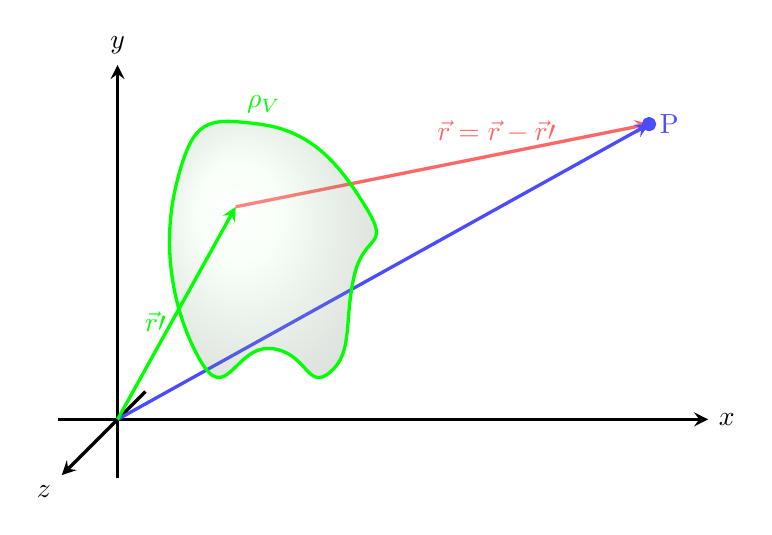
\begin{tikzpicture}[line width = 1.2pt, line join=round,x=1.5cm,y=1.5cm,z={(-0.35355cm,-0.35355cm)},>=stealth]
	% Koordinatensystem
	\draw [->] (-0.5,0) -- (5,0) node[anchor=west] {$x$};
	\draw [->] (0,-0.5) -- (0,3) node[anchor=south] {$y$};
	\draw [->] (0,0,-1) -- (0,0,2) node[anchor=north east] {$z$};
	% Differenzvektor R
	\draw [->, color=red!60] (1,1.8) -- (4.5,2.5);
	\draw [color=red!60] (3.8,2.25) node[anchor=south east] {$\vec{r}  = \vec{r}  - \vec{r}\prime  $};
	% Aufpunkt
	\draw [->,color=blue!70] (0,0) -- (4.5,2.5) node[anchor=west] {$\mathrm{P} $};
	\filldraw [color=blue!70] (4.5,2.5) circle (2pt);
	% Ladungsdichte
	\coordinate (a) at (2.1,1.8);
	\coordinate (b) at (2,1.2);
	\coordinate (c) at (1.8,0.4);
	\coordinate (d) at (1.3,0.6);
	\coordinate (e) at (0.7,0.5);
	\coordinate (f) at (0.5,2);
	\coordinate (g) at (1.2,2.5);
	\shade[ball color=white!10!green!20,opacity=0.20] plot [smooth cycle, tension = 1] coordinates {(a) (b) (c) (d) (e) (f) (g)};
	\draw [color=green] plot [smooth cycle, tension = 1] coordinates {(a) (b) (c) (d) (e) (f) (g)} node [sloped, above] {\ $ \rho_\text{V} $};
	\draw [->,color=green] (0,0) -- (1,1.8);
	\draw [color=green] (0.5,1.0) node[anchor=north east] {$ \vec{r}\prime  $};
\end{tikzpicture}
	  \end{center}
	  Abgesehen davon ist der Raum entweder ein \textbf{Vakuum} mit $\varepsilon=\varepsilon_{0}$
	  oder kann als \textbf{perfekt leitend} $\kappa \to\infty$ angesehen werden.
	   Für solche ideal leitenden Gebiete gilt, dass die Relaxation der freien Ladungsträger näherungsweise sofort stattfindet ($\nearrow$\ref{relax}). Alle elektrischen Felder werden also praktisch instantan kompensiert:
	  \begin{equation}\begin{split}
			  \vec{E}= \vec{0}\text{ in den perfekt leitenden Gebieten}
		  \end{split}\end{equation}
	  \textbf{Gesucht} ist häufig das Feld im Raum außerhalb der perfekten Leiter und der Ladungsanordnung.\\
Aus \ref{GGes2} folgt im Vakuum ($\varepsilon=\varepsilon_{0}$)
\begin{equation}
			  \div \vec{D}  = \div \left( \varepsilon_0 \cdot \vec{E} \right) = \rho_\text{V} \quad\quad\quad \vec{E} \cdot \dd\vec{A}              =
			  \iiint\limits_{V} \rho_\text{V} \dd V
			  = Q \text{ in }V
\end{equation}
  \subsection{Coulomb-Integral}
  Coulomb-Integral $\neq$ Coulomb-Gauss-Integral!
	  \subsubsection{Nutzung zur Berechnung des $E$-Feldes}
			   Die Berechnung des E-Feldes aus dem
			        \textbf{Coulomb-Gauss-Integral}
			        \begin{equation}\begin{split}
					        \oiint\limits_{O(V)}
					        \vec{E} \cdot \dd\vec{A} = \frac{1}{\varepsilon_0}
					        \iiint\limits_{V} \rho_\text{V} \dd V
				        \end{split}\end{equation}
			        ist ein guter und intuitiver Lösungsweg, wenn das \textbf{linke Integral}
			        leicht zu einem Ausdruck für $\vec{E}(\vec{r} )$ für alle
			        $\vec{r} $ im Lösungsvolumen umgeformt werden kann.
			   Ob das \textbf{rechte Integral} dann \textbf{analytisch}
			        gelöst werden kann, ist grundsätzlich sekundär.
			   Eine
			        analytische Lösung ist zwar in jedem Fall vorzuziehen, aber im
			        Zweifel kann as Integral immer \textbf{numerisch} gelöst
			        werden.
			   Leider kann das \textbf{linke Integral} jedoch nur
			        ausgewertet werden, wenn \textbf{starke Symmetrien} vorliegen. Ein Beispiel dafür ist:\\\\
			        \textbf{Kugelsymmetrische Ladungsverteilung am Ursprung:}\\
			        Das $E$-Feld ist radial gerichtet, die Werte sind nur vom Betrag $r'$ abhängig.
			        \begin{equation}\begin{split}
			        		\rho_\text{V} (\vec{r}' ) =  \rho_\text{V}(r') \qquad \vec{E} (\vec{r}' ) = E(r')\vec{e_{r'}}
			        \end{split}\end{equation}
			        Das Volumen (hat die Symmetrie des ursprünglichen Problems) kann besonders einfach gewählt werden - $V$ ist eine Kugel mit Radius r um den Ursprung. Daraus folgt: $\dd\vec{A} =
			        \dd A \vec{e_{r'}}   \rightarrow \vec{\bm{E}} \cdot
			        \textbf{d}\vec{\bm{A}} = \bm{E(r) \textbf{d} A}$. Außerdem lässt sich $E(r)$ vor das Integral ziehen, weil für alle Punkte auf einer Kugeloberfläche die Feldstärke aus Symmetriegründen konstant sein muss. 
			        \begin{equation}\begin{split}
			        		\oiint\limits_{O(V)}
			        		\vec{E} \cdot \dd\vec{A} = & E(r) \oiint\limits_{O(V)}
			        		\dd A = 4\pi r^2 E(r) \\
			        		= & \frac{1}{\varepsilon_0} \iiint\limits_{V}
			        		\rho_\text{V} \dd V =  \frac{1}{\varepsilon_0} \int\limits_0^r \rho_\text{V}(r') r'^2\dd r'
			        		\int\limits_0^{2\pi} \dd \varphi \int\limits_0^\pi \sin\vartheta
			        		\dd\vartheta \\
			        		= & \frac{4\pi}{\varepsilon_0}\int\limits_0^r \rho_\text{V}(r') r'^2\dd r'\\
			        		E(r) = & \frac{1}{\varepsilon_0 r^2} \int\limits_0^r \rho_\text{V}(r') r'^2\dd r'
			        \end{split}\end{equation}
			        Das Ergebnis ist allgemeingültig für alle kugelsymmetrischen Ladungsverteilungen am Urspurung. Betrachtet man nun eine homogen geladene Kugel mit Radius $R$ und keiner Ladung außerhalb folgt (wegen der Fallunterscheidung muss man für den zweiten Bereich das Integral in zwei Integrale $0\to R, R\to r$ spalten):
			        \begin{equation}\begin{split}
			        		\rho_\text{V} (\vec{r}' ) = \begin{cases}
			        			\rho_\text{V} & \text{ für } r' \le R \\
			        			0      & \text{ für } r' > R
			        		\end{cases};\quad E(r) =  \begin{cases}
			        			\frac{\rho_\text{V}}{\varepsilon_0r^2}\frac{1}{3}r^3 =
			        			\frac{\rho_\text{V}}{3\varepsilon_0}r= \frac{Q r}{4\pi\varepsilon_0 R^3}              & \text{ für } r \le R \\
			        			\frac{\rho_\text{V}}{\varepsilon_0r^2}\frac{1}{3}R^3 = \frac{Q}{4\pi\varepsilon_0r^2} & \text{ für } r > R
			        		\end{cases}
			        \end{split}\end{equation}
			        Es fällt auf, dass das Feld außerhalb der kugelsymmetrischen Ladungsanordnung wie das einer Punktladung aussieht.\\\\
			   \textbf{Weitere Beispiele}:
			        \begin{itemize}
				        \item geladener Ring
				        \item unendlich langer, homogen geladener Zylinder
			        \end{itemize}
	  \subsubsection{Skalarpotential}
	  \textbf{Empirisch gilt:}\\ 
			   Für die \textbf{Überlagerung} (Superposition $\rightarrow$ Maxwell-Gleichungen sind lineare Gleichungen $\Rightarrow$ Summen von Lösungen der Maxwell-Gleichungen sind wiederum eine Lösung der Maxwell-Gleichungen) von $n$
			        einzelnen Punktladungen $q_j$ an Positionen $\vec{r} _j$ ist
			        das Feld bekannt, falls keine weiteren
			        \textbf{Randbedingungen im Endlichen} (im wesentlichen freier Raum betrachtet) vorliegen:
			        \begin{equation}\begin{split} 
					        \vec{E} (\vec{r} )= \frac{1}{4\pi\varepsilon_0} \sum_{j=1}^n \frac{q_j\left(\vec{r} -\vec{r} _j\right)}{\left|\vec{r} -\vec{r} _j\right|^3}
				        \end{split}\end{equation}
			   Beim Übergang auf eine \textbf{kontinuierliche
				        Ladungsverteilung} mit dem Volumenelement $\dd^3r'$
			        \begin{equation}\begin{split}
					        \dd q =
					        \rho_\text{V}(\vec{r}' )\dd^3r'\end{split}\end{equation}

			        ergibt sich sofort das \textbf{Coulomb-Integral}

			        \begin{equation}\label{CoulInt}\begin{split}
					        \boxed{\vec{E} (\vec{r} )= \frac{1}{4\pi\varepsilon_0}
					        \int
					        \frac{\rho_\text{V}(\vec{r}' )\left(\vec{r} -\vec{r}' \right)}{\left|\vec{r} -\vec{r}' \right|^3
					        } \dd^3r'}
				        \end{split}\end{equation}
			   Außerdem gilt
			        \begin{equation}\begin{split}
					        \frac{\vec{r} -\vec{r}' }{\left|\vec{r} -\vec{r}' \right|^3}
					        = -\grad  \frac{1}{\left|\vec{r} -\vec{r}' \right|}
				        \end{split}\end{equation}
			   und somit (Gradient und Integration vertauschen $\rightarrow$ Linearität!)
			        \begin{equation}\label{PotR}\begin{split}
					        \vec{E}(\vec{r} ) = -\grad \phi \quad\text{mit}\quad
					        \boxed{\phi(\vec{r} ) = \frac{1}{4\pi\varepsilon_0}
						        \int
						        \frac{\rho_\text{V}(\vec{r}' )}{\left|\vec{r} -\vec{r}' \right|} \dd^3r'} \quad\text{als }\textbf{{Skalarpotential}}
				        \end{split}\end{equation}
			        Das Skalarpotential kann also auch aus dem bekannten $E$-Feld einer Punktladung berechnet werden.\\\\
\textbf{Formal gilt:}\\ 
	  Mit \ref{poin} folgt: \begin{equation}\boxed{\rot \vec{E} = \vec{0} \Rightarrow \vec{E}
			  = -\grad \phi}\end{equation}
		  Das \enquote{-} ist eine Konvention und $\phi$ das
	  \textbf{elektrische Skalarpotential}.
	  \subsection{Poisson- und Laplace-Gleichung}
 Für statische Probleme gilt immer $\rot \vec{E} = \vec{0}$. Daher folgt aus \ref{poin} immer $\vec{E} = - \grad \phi$. Für \textbf{einfache} Medien mit $\vec{D}  = \varepsilon \vec{E}$ gilt mit \ref{GGes2} $\div \vec{E} =
			        \frac{1}{\varepsilon} \rho_\text{V} $. Einsetzen liefert:
		        \begin{align}
			        \nonumber\div \vec{E} =                                             &
			        \frac{1}{\varepsilon} \rho_\text{V}                                                             \\
			       \nonumber \div \left(-\grad \phi\right) =                            & \frac{1}{\varepsilon}
			        \rho_\text{V}                                                                                   \\
			       \Aboxed{ \Delta \phi =                                              & - \frac{1}{\varepsilon}
			        \rho_\text{V}    }                                          & \textbf{
			        Poisson-Gleichung}                                                                              \\
			        \text{Spezialfall } \rho_\text{V}=0 \to\quad \Aboxed{\Delta \phi = & 0    }                   & \textbf{
				        Laplace-Gleichung}
		        \end{align}
		   Ist $\phi$ die Lösung des Problems, erfüllt
		        das zugehörige $\vec{E} = - \grad \phi$ \textbf{automatisch} die
		        zweite Gleichung $\rot \vec{E} = \vec{0}$
		   Allerdings ist nun anstelle von zwei DGLs erster Ordnung nun
		        eine \textbf{DGL zweiter Ordnung} zu lösen.
		    Bei der Gradientenbildung spielt eine Konstante keine Rolle($\vec{E}(\phi + \text{const.}) =
			        \vec{E}(\phi)$), das heißt $\phi$ nur bis auf additive
		        Konstante bestimmt. Für das Feld macht ein konstanter Offset vom Skalarpotential keinen Unterschied.

  \subsection{Kraft und Arbeit, Feldlinien und Äquipotentialflächen}
		   Die Kraft auf eine Probeladung $q$ im Feld $\vec{E}(\vec{r} )$ ist gegeben als (Coulomb-Kraft)
		        \begin{equation}\begin{split}
				        \vec{F}(\vec{r} ) = q \vec{E}(\vec{r} )
			        \end{split}\end{equation}
		   Lässt man eine fiktive Testladung (positiv) im Feld los, dann wirkt auf sie eine Kraft. Deshalb fängt sie sich an zu bewegen. Die \textbf{Trajektorie} beschreibt eine \textbf{Feldlinie} (Orientierung: von \enquote{+}
		        nach \enquote{-}). Orte mit gleichem Skalarpotential bilden eine
		        \textbf{Äquipotentialfläche}.
		   Sei $\dd\vec{s}$ eine kleine Verschiebung auf einer
		        Äquipotentialfläche, dann gilt:
		        \begin{align*}
				        \dd \phi = & \phi(\vec{r} +\dd\vec{s}) - \phi(\vec{r} ) \equiv 0\quad &&\text{ (Potential ändert sich nicht)}\\
				        0= & \grad \phi \cdot \dd\vec{s}  &&\nearrow \text{\ref{totDiff}, totales Differential}
			        \end{align*}
		        Daraus folgt, dass die Feldlinien senkrecht auf den Äquipotentialflächen ($\dd\vec{s}$ ist ein Vektor in der Äquipotentialfläche) stehen:
		        \begin{equation}\begin{split}
				        \grad \phi \perp \dd\vec{s} \land \grad \phi \parallel \vec{E} \to
				        \boxed{\vec{E} \text{(Feldlinien)} \perp \text{Äquipotentialflächen}}
			        \end{split}\end{equation}

	  \subsubsection{Wegunabhängigkeit}
		  \begin{center}
	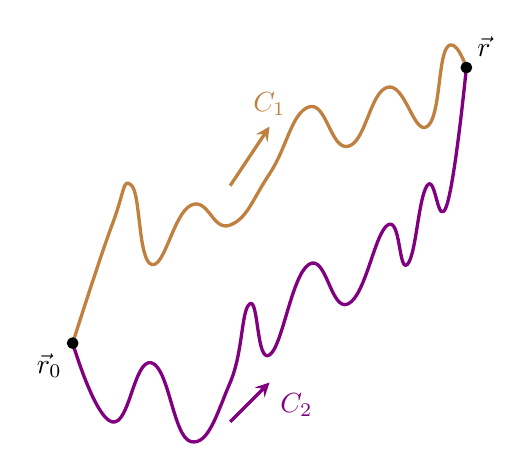
\begin{tikzpicture}[line width = 1.2pt, line join=round,x=0.5cm,y=0.5cm,>=stealth]
		% Koordinaten der Punkte
		\coordinate (a) at (0,0);
		\coordinate (b) at (10,7);
		% Weg 1
		\draw [color=brown] plot[smooth,tension=0.8] coordinates{(a) (1,3) (1.5,4) (2,2) (3,3.5) (4,3) (5,4.3) (6,6) (7,5) (8,6.5) (9,5.5) (9.5,7.5) (b)};
		\draw[->,color=brown] (4,4) -- (5,5.5) node[anchor=south] {$C_1$};
		% Weg 2
		\draw [color=violet] plot[smooth, tension=0.8] coordinates{(a) (1,-2) (2,-0.5) (3,-2.5) (4,-1) (4.5,1) (5,-0.3) (6,2) (7,1) (8,3) (8.5,2) (9,4) (9.5,3.5) (b)};
		\draw[->,color=violet] (4,-2) -- (5,-1) node[anchor=north west] {$C_2$};
		% Punkt 0
		\filldraw (a) circle (1.5pt);
		\draw (a) node[anchor=north east] {$\vec{r} _0$};
		% allgemeiner Punkt
		\filldraw (b) circle (1.5pt);
		\draw (b) node [anchor = south west] {$\vec{r} $};
	\end{tikzpicture}
	\hfill
	\begin{tikzpicture}[line width = 1.2pt,
			line join=round,
			scale=1,
			x=0.5cm,
			y=0.5cm,
			>=stealth]
		% Koordinaten der Punkte des Weges
		\coordinate (a) at (0,2);
		\coordinate (b) at (8,5);
		\coordinate (c) at (2,3);
		\coordinate (d) at (-2,4.3);
		\coordinate (e) at (9.6,2.5);

		% Rechte Winkel
		\draw (0.6,2.4) arc (10:120:0.4cm);
		\filldraw (0.05,2.6) circle (1pt);
		\draw (7.7,5.8) arc (120:210:0.4cm);
		\filldraw (7.62,5.2) circle (1pt);
		% Fläche 1
		\draw plot[smooth, tension = 0.8] coordinates{(-3,5) (a) (0,-2)};
		\draw [decorate, decoration={markings,
					mark=between positions 0.2 and 0.5 step 3mm with
						{\arrow[green]{latex}}}] plot[smooth, tension = 0.8] coordinates{(-3,5) (a) (0,-2)};
		\draw (0,-2) node[anchor=north] {$\phi(\vec{r} _0)$};
		% Fläche 2 
		\draw  plot[smooth, tension = 0.8] coordinates{(7,8) (b) (e) (10,2)};
		\draw  [decorate, decoration={markings,
					mark=between positions 0.6 and 0.95 step 3mm with
						{\arrow[green]{latex}}}] plot[smooth, tension = 0.8] coordinates{(7,8) (b) (e) (10,2)};
		\draw (10,2) node[anchor=north west] {$\phi(\vec{r} )$};
		% Punkte
		\draw (a) circle (1.5pt);
		\draw (a) node[anchor=north east] {$\vec{r} _1$};
		\draw (b) circle (1.5pt);
		\draw (b) node[anchor=south west] {$\vec{r} _2$};
		\draw (d) circle (1.5pt);
		\draw (d) node[anchor=south west] {$\vec{r} _0$};
		%\draw [color=green] plot[smooth] coordinates{(d) (f) (a)}; 

		\draw (e) node[anchor=north east] {$\vec{r} $};
		\draw (e) circle (1.5pt);

		% Weg
		\draw [color=magenta] plot[smooth, tension=0.8] coordinates{(a) (c) (6,4) (b)};
		\draw [decorate, , decoration={markings,
					mark=between positions 0.1 and 0.99 step 3mm with
						{\arrow[green]{latex}}}] plot[smooth, tension=0.8] coordinates{(a) (c) (6,4) (b)};
		\draw [->,color=magenta] (c) -- ++(3,{2/5*3}) node[anchor=south] {$\vec{E}$};
		\draw [->,color=blue] (c) -- ++(2,{2/5*2}) node[anchor=south east] {$\dd \vec{s}$};
	\end{tikzpicture}
\end{center}
			   Es werden zwei beliebige Wege $C_1$ und $C_2$ zwischen
			        $\vec{r} _0$ und $\vec{r} $ betrachtet.
			   Wegen $\rot \vec{E} =\vec{0} $ gilt für jeden geschlossenen
			        Weg $C$:
			        $
				        \oint\limits_C \vec{E}\cdot\dd\vec{s} = 0
			        $.
			   Der Weg $C_1 + (-C_2)$ ist ein geschlossener Weg. Daher
			        folgt die \textbf{Wegunabhängigkeit}:
			        \begin{equation}\begin{split}
					        \boxed{\int\limits_{\vec{r} _0, C_1}^{\vec{r} } \vec{E}\cdot\dd\vec{s} =        \int\limits_{\vec{r} _0, C_2}^{\vec{r} } \vec{E}\cdot\dd\vec{s}}
				        \end{split}\end{equation}
			   Außerdem gilt, dass Wege auf der Äquipotentialfläche ($\vec{r} _0\to\vec{r} _1$ und
			        $\vec{r} _2\to\vec{r} $) tragen nicht bei, da $\dd\vec{s}
				        \perp \vec{E}$ gilt.
			   Auf Wegen entlang einer Feldlinie ($\vec{r} _1\to\vec{r} _2$) kann man vereinfachen
			        $\vec{E}\cdot\dd\vec{s} = E \dd s = -|\grad \phi| \dd s$.
			   Somit folgt (siehe auch \ref{totDiff}):
			        \begin{equation}\begin{split}
					        \boxed{\int\limits_{\vec{r} _0}^{\vec{r} } \vec{E}\cdot\dd\vec{s} =
						        -
						        \int\limits_{\vec{r} _1}^{\vec{r} _2}
						        |\grad \phi|\dd
						        s
						        =
						        \phi(\vec{r} _0)
						        - \phi(\vec{r} )}
				        \end{split}\end{equation}
	  \subsubsection{Spannung}
		  Man definiert die
		  \textbf{Spannung} $U_{21}$ als \textbf{Potentialdifferenz}:
		  $$
			  U_{21} = \phi_2 - \phi_1 = - \int\limits_{\vec{r} _1}^{\vec{r} _2}
			  \vec{E}\cdot \dd \vec{s}
		  $$
	  \subsubsection{Arbeit}
		  Auf eine Probeladung $q$ wirkt im $E$-Feld die elektrostatische
		  Kraft $\vec{F}_e = q\vec{E}$. Um die Ladung am Ort
		  festzuhalten ist eine gegengerichtete Kraft aufzuwenden
		  $\vec{F}_\text{mech} = -\vec{F}_e$. Die \textbf{Arbeit} $A$
		  auf dem Weg von $\vec{r} _1$ nach $\vec{r_2}$ ist somit
		  \begin{equation}\begin{split}
				  A = \int\limits_{\vec{r} _1}^{\vec{r} _2}
				  \vec{F}_\text{mech}\cdot\dd\vec{s} = - \int\limits_{\vec{r} _1}^{\vec{r} _2}
				  \vec{F}_e\cdot\dd\vec{s} = -q\int\limits_{\vec{r} _1}^{\vec{r} _2}
				  \vec{E}\cdot\dd\vec{s} = q (\phi(\vec{r} _2)-\phi({\vec{r} _1)})
				  = q U_{21}
			  \end{split}\end{equation}
	  \subsubsection{Elektrostatische Energie}
		  Die \textbf{Energie} einer auf einen \textbf{endlichen Raum} beschränkten
		  Ladungskonfiguration $\rho_\text{V}$ entspricht der Arbeit, um
		  Ladungen aus dem Unendlichen zu dieser Konfiguration zu bringen. Wegen $\phi(\vec{r} ) =
			  \frac{1}{4\pi\varepsilon_0}\int\frac{\rho_\text{V}(\vec{r}' )}{\left|\vec{r} -\vec{r}' \right|}
			  \dd^3r$ ist \textbf{$\phi(\infty) = 0$} für eine räumlich begrenzte Ladungsverteilung.
			  Betrachtet werden $N$ Punktladungen. Nun wird das Potential am Ort $\vec{r} _i$ der $i$-ten Punktladung herrührend von den ersten $(i-1)$ Punktladungen mit Ladung $q_j$ an den Orten $\vec{r} _j$ betrachtet:
			        $$
				        \phi(\vec{r} _i) = \frac{1}{4\pi\varepsilon_0} \sum_{j=1}^{i-1}
				        \frac{q_j}{|\vec{r} _i - \vec{r} _j|}
			        $$
			       Die Arbeit, die benötigt wird, um die Ladung $q_i$ von $\infty$ nach $\vec{r} _i$ zu bewegen ist $A_i = q_i\phi(\vec{r} _i)$.
			        Die Gesamtarbeit $A = \sum_{i=2}^N A_i$ (der Term für $i=1$
			        verschwindet, da der Raum bei der Verlagerung der ersten Ladung
			        noch feldfrei ist) entspricht der \textbf{elektrostatischen
				        Energie} $W_\text{e}$:
			        \begin{equation}\begin{split}A = W_\text{e} = \frac{1}{4\pi\varepsilon_0} \sum_{i=2}^N \sum_{j=1}^{i-1}
					        \frac{q_i q_j}{|\vec{r} _i - \vec{r} _j|} = \frac{1}{\bm{8}\pi\varepsilon_0} \sum_{i=1}^N \sum_{j=1}^{N}
					        \frac{q_i q_j}{|\vec{r} _i - \vec{r} _j|} \bm{(1-\delta_{ij})}
				        \end{split}\end{equation}
			   In der Formel für $N$ Punktladungen tauchen die Terme $i=j$ nicht auf (Vorstellung über Dreiecksmatrix). Beim Übergang auf kontinuierliche Ladungsverteilungen
			        lassen sie sich aber nicht ausschließen. Der \textbf{nicht
				        völlig äquivalente} Ausdruck heißt in diesem Fall somit:
			        \begin{equation}\label{elstatE}\begin{split}
					        \boxed{ W_\text{e} = \frac{1}{8\pi\varepsilon_0} \iint
						        \frac{\rho_\text{V}(\vec{r} ) \rho_\text{V}(\vec{r}' )}{|\vec{r} -
							        \vec{r}' |} \dd^3 r\dd^3 r' = \frac{1}{2} \int
						        \rho_\text{V}(\vec{r} )\phi(\vec{r} ) \dd^3 r}
				        \end{split}\end{equation}
			   Die Diskussion des Unterschieds führt zum Begriff der
			        \textbf{Selbstenergie} einer Punktladung, der jedoch (bisher) nicht
			        widerspruchsfrei aufgeklärt werden kann. Das ist nicht völlig
			        überraschend, da Punktladungen nur Modelle sind.
			   Mit $\rho_\text{V}=-\varepsilon_0\Delta \phi$ und
			        $\div (\phi\grad \phi) = \grad \phi\grad \phi + \phi\Delta \phi$
			        folgt nach Einsetzen in \ref{elstatE}:
			        \begin{equation}\begin{split}
					        W_\text{e} = & -\frac{\varepsilon_0}{2}\left(\underbrace{\int \div (\phi\grad \phi)
					        \dd^3 r}_0 - \int (\grad \phi)^2 \dd^3 r\right)  =
					        \frac{\varepsilon_0}{2} \int (\grad \phi)^2 \dd^3 r\\
					        = & \frac{\varepsilon_0}{2} \int |\vec{E}|^2 \dd^3 r
					        \quad\textbf{Energiedichte:} \boxed{w_\text{e} = \frac{\varepsilon_0}{2} |\vec{E}|^2}
				        \end{split}\end{equation}
			        	Eine ganz analoge Herleitung ergibt das \textbf{verallgemeinerte Resultat} für Materie ($\nearrow$\ref{materie}), nach \ref{DEMat} ist hier der $D,E$-Zusammenhang etwas komplizierter:
			        	\begin{equation}\label{edichteE}\begin{split}
			        			\boxed{W_\text{e} = \frac{1}{2}\int \vec{E}\cdot\vec{D} \dd^3 r}
			        			\quad\textbf{Energiedichte:} \boxed{w_\text{e} = \frac{1}{2} \vec{E}\cdot\vec{D}}
			        	\end{split}\end{equation}
 \section{Monopol bis Multipolentwicklung}
  Siehe auch $\nearrow$EMF für einfache Spezialfälle (Plattenkondensator, Kugelkondensator, Zylinderkondensator).
	  Die \textbf{Lösungsstrategie} ist dort immer gleich:
	        \begin{enumerate}
		        \item geeignetes Koordinatensystem wählen
		        \item idealisieren: Randeffekte vernachlässigen
		        \item Symmetrie: Feldrichtung überlegen
		        \item E-Feld berechnen (z.B. Coulomb-Gauß)
		        \item Räumlich beschränkte Ladungsverteilung $\implies$ Potential
		              im Unendlichen verschwindet
		        \item[$\to$] Potential, Spannung, Kapazität $C = Q/U$,
		              Energiedichte, Energie
	        \end{enumerate}
  \subsection{Monopol}
  Ein Monopol ist eine Punktladung $q$ am Ort $\vec{r_0}$.\\
	  \begin{minipage}{0.5\textwidth}
		  \begin{center}
	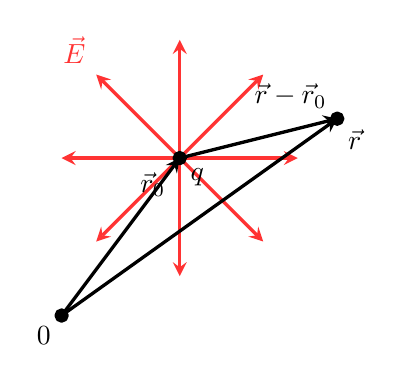
\begin{tikzpicture}[line width = 1.2pt, line join=round,x=1cm,y=1cm,>=stealth]
		% Koordinatensystem
		%\draw [->] (-2,0) -- (2,0) node[anchor=west] {$x$};
		%\draw [->] (0,-2) -- (0,2) node[anchor=south] {$y$};
		% elektrisches Feld
		\draw [<->,color=red!80] (-1.5,0) -- (1.5,0);
		\draw [<->,color=red!80] (0,-1.5) -- (0,1.5);
		\draw [<->,color=red!80] (-1.06066,-1.06066) -- (1.06066,1.06066);
		\draw [<->,color=red!80] (-1.06066,1.06066) -- (1.06066,-1.06066);
		\draw [color=red!80] (-1.06066,1.06066) node[anchor=south east]{$\vec{E}$};
		%\draw [color=red!40,style=dashed] (0,0) circle (1.5);
		% Aufpunkt
		\draw [->,color=black] (-1.5,-2) -- (2,0.5) node[anchor=north west]{$\vec{r} $};
		\draw [->,color=black] (-1.5,-2) -- (0,0) node[below left=1.3]{$\vec{r} _0$};
		\draw [->,color=black] (0,0) -- (2,0.5) node[above left=-0.1]{$\vec{r} -\vec{r} _0$};
		\filldraw [color=black] (2,0.5) circle (2pt);
		\filldraw [color=black] (-1.5,-2) circle (2pt);
		\draw [color=black] (-1.5,-2)  node[anchor=north east]{$0$};
		%\draw [color=black] (1.5,1.5) node[anchor=north east] {$\vec{r} $};
		% Ladung
		\filldraw [color=black] (0,0) circle (2pt);
		\draw [color=black] (0,0) node[anchor=north west]{$q$};
	\end{tikzpicture}
\end{center}

	  \end{minipage}
	  \begin{minipage}{0.5\textwidth}
		  \begin{align}
			  \vec{E}(\vec{r} ) = & \frac{1}{4\pi\varepsilon_0} q\frac{\vec{r} -\vec{r} _0}{|\vec{r} -\vec{r} _0|^3} \\
			  \phi (\vec{r} ) =   & \frac{1}{4\pi\varepsilon_0} q\frac{1}{|\vec{r} -\vec{r} _0|}
		  \end{align}
	  \end{minipage}
  \subsection{Dipol}\label{Dipol}
  Ein Dipol besteht aus zwei Punktladungen $+q$ und $-q$ mit Distanz $\vec{a}$.\\
	  \begin{minipage}{0.5\textwidth}
		  \begin{center}
	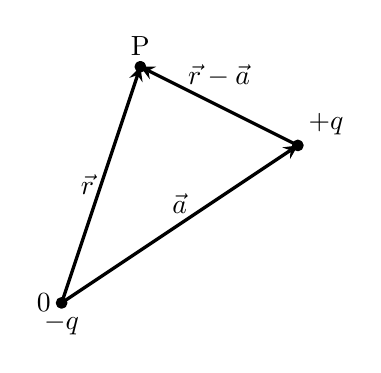
\begin{tikzpicture}[line width = 1.2pt, line join=round,x=1cm,y=1cm,>=stealth]
		% Achsen
		%\draw [->,dashed] (0,0) -- (4,0) node[anchor=north west] {$x$};
		%\draw [->,dashed] (0,0) -- (0,4) node[anchor=south east] {$y$};
		\draw (0,0) node[anchor=east] {$0$};
		% Koordinaten für die Ladungen
		\coordinate (a) at (0,0);
		\coordinate (b) at (3,2);
		% Koordinaten für den Raumpunkt
		\coordinate (c) at (1,3);
		% Vektor a
		\draw [->,color=black] (a) -- (b);
		\draw [color=black] (1.5,1) node[anchor = south] {$\vec{a}$};
		% Vektor r
		\draw [->,color=black] (0,0) -- (c);
		\draw [color=black] (0.55,1.5) node [anchor=east] {$\vec{r} $};
		% Vektor r-a
		\draw [->,color=black] (b) -- (c);
		\draw [color=black] (2,2.6) node[anchor=south] {$\vec{r}  - \vec{a}$};
		% partielle Ladungen
		\filldraw [color=black] (a) circle (1.5pt);
		\draw [color=black] (a) node[anchor=north] {$-q$};
		\filldraw [color=black] (b) circle (1.5pt);
		\draw [color=black] (b) node[anchor=south west] {$+q$};
		% Beobachtungspunkt
		\filldraw [color=black] (c) circle (1.5pt);
		\draw [color=black] (c) node[anchor= south] {$\mathrm{P} $};
	\end{tikzpicture}
\end{center}
	  \end{minipage}
	  \begin{minipage}{0.5\textwidth}
			  Konventionsgemäß wird der Abstandsvektor $\vec{a}$ von \enquote{-} nach \enquote{+} definiert. Das \textbf {Dipolmoment} ist definiert als $\vec{p} = q\cdot\vec{a}$ (wenn $a=0$ kompensieren sich die Ladungen und es gibt gar kein Feld). $-q$ wird in den Ursprung gelegt. Der Beobachtungspunkt ist $P$. Die Superposition zweier Monopole liefert das Feld und Potential.
	  \end{minipage}

	  \begin{equation}\begin{split}
			  \vec{E}(\vec{r} ) =  \frac{1}{4\pi\varepsilon_0} \left( -q\frac{\vec{r} }{|\vec{r} |^3}  + q\frac{\vec{r} -\vec{a}}{|\vec{r} -\vec{a}|^3}  \right) \quad\quad\quad \phi (\vec{r} ) =  \frac{1}{4\pi\varepsilon_0} \left( -q\frac{1}{|\vec{r} |}  + q\frac{1}{|\vec{r} -\vec{a}|} \right)
		  \end{split}\end{equation}
	  Im folgenden Bild sieht man Feldlinien und Äquipotentialflächen an einem Dipol.
	  \begin{center}
		  \resizebox{0.5\textwidth}{!}{

			  \input{res/dipol-feld.pgf}
		  }
	  \end{center}
	  \subsubsection{Potential des Dipols - Taylorentwicklung}
			  Der Ausdruck für das Potential $\phi (\vec{r} ) =  \frac{1}{4\pi\varepsilon_0} \left( -q\frac{1}{|\vec{r} |}  + q\frac{1}{|\vec{r} -\vec{a}|} \right)$ ist einfacher. Deshalb wird dieser Term weiter betrachtet.
			  Die \textbf{Taylorentwicklung} nach \ref{TaylorSkalar} von $\frac{1}{|\dots|}$ am Punkt $\vec{r} $ in Richtung $-\vec{a}$ ist:
			        \begin{equation}\label{Taylrrr}\begin{split}
					        \boxed{\frac{1}{|\vec{r} -\vec{a}|} = \frac{1}{r} + \frac{\vec{r} \cdot\vec{a}}{r^3} + \frac{1}{2} \frac{3(\vec{r} \cdot\vec{a})^2-r^2a^2}{r^5} + \ldots }
				        \end{split}\end{equation}
			  Bei der Entwicklung des Potentials entfällt der Term $1/r$, da er sowohl bei $+q$ als auch bei $-q$ vorkommt:
			        \begin{equation}\label{TaylorDip}\begin{split}
					        \phi (\vec{r} ) =  \frac{q}{4\pi\varepsilon_0} \left[ \frac{\vec{r} \cdot\vec{a}}{r^3} + \frac{3(\vec{r} \cdot\vec{a})^2-r^2a^2}{2r^5} + \ldots \right]
				        \end{split}\end{equation}
	  \subsubsection{Punktdipol - Dipolmoment als lokale Größe}
	 Bisher ist $\vec{a}$ eine endliche Größe und das Dipolmoment $\vec{p} = q \vec{a}$ somit nicht nur einem Raumpunkt zugeordnet. Ein Punktdipol als Modell ist aber sehr hilfreich. Für $\vec{a}\to \vec{0}$ muss gleichzeitig $q\to\infty$ gehen, damit $\lim \limits_{\vec{a}\to \vec{0}}\vec{p} =\vec{p}$ bleibt (sonst kompensieren sich die gleich großen Ladungen einfach). Dieser Übergang führt zum \textbf{Potential des Punktdipols} $\phi_D$, wobei die Terme $qa^2$, $qa^3$, ... in \ref{TaylorDip} wegen des Grenzübergangs vernachlässigt werden können ($\lim\limits_{\substack{a\to 0\\q\to\infty}}qa^2=p\lim\limits_{a\to 0} a=0$):
			        \begin{equation}\begin{split}
					        \boxed{\phi_D(\vec{r} ) = \frac{1}{4\pi\varepsilon_0} \frac{\vec{r} \cdot\vec{p}}{r^3} = -\frac{1}{4\pi\varepsilon_0} \vec{p}\cdot\grad \frac{1}{r} }
				        \end{split}\end{equation}
			  Die weitere Berechnung erfolgt in Kugelkoordinaten mit der Festlegung $\vec{p}\parallel\vu{z}$, wodurch die Auswertung des Skalarproduktes $\vec{r} \cdot\vec{p} = r p \cos\vartheta$ besonders einfach ist.
			        \begin{equation}\begin{split}
					        \boxed{\phi_D(\vec{r} ) = \frac{1}{4\pi\varepsilon_0} \frac{p\cos\vartheta}{r^2} }
				        \end{split}\end{equation}
			  Das Feld folgt aus $\vec{E}_D = -\grad \phi_D $ (Berechnung $\nearrow$ \ref{difOpKo}):
			        \begin{equation}\begin{split}
					        \boxed{E_{D,r} = \frac{p}{4\pi\varepsilon_0} \frac{2\cos\vartheta}{r^3}, \quad E_{D,\vartheta} = \frac{p}{4\pi\varepsilon_0} \frac{\sin\vartheta}{r^3}, \quad E_{D,\varphi} = 0 }
				        \end{split}\end{equation}
			  Koordinatenfrei gilt (Angabe ohne Herleitung, Achtung Dipol hierfür immernoch am Ursprung!):
			        \begin{equation}\begin{split}
					        \boxed{\vec{E}_{D} = \frac{1}{4\pi\varepsilon_0}\left[ \frac{3(\vec{r} \cdot\vec{p}) \vec{r} }{r^5} -\frac{\vec{p}}{r^3} \right]}
				        \end{split}\end{equation}
	  \subsubsection{$N$ diskrete Dipole, Dipoldichte}
			  Das Potential (und Feld) von $N$ Dipolen $\vec{p}_j$ bei $\vec{r} _j$ folgt einfach aus Superposition:
			        \begin{equation}\begin{split}
					        \phi_D(\vec{r} ) = \frac{1}{4\pi\varepsilon_0} \sum_{j=1}^N \frac{\vec{p}_j\cdot ( \vec{r} -\vec{r} _j)}{|\vec{r} -\vec{r} _j|^3} = -\frac{1}{4\pi\varepsilon_0} \sum_{j=1}^N \vec{p}_j\cdot \grad _r \frac{1}{|\vec{r} -\vec{r} _j|}
				        \end{split}\end{equation}
			   Der Übergang zu einer kontinuerlichen \textbf{Dipoldichte} $\vec{m}(\vec{r} )$ (Definition über: $\vec{p} = \int\limits_V \vec{m}(\vec{r}' )\dd^3 r'$) folgt mit:
			        \begin{equation}\begin{split}
					        \phi_D(\vec{r} ) = \frac{1}{4\pi\varepsilon_0} \int\limits_V \frac{\vec{m}(\vec{r}' )\cdot ( \vec{r} -\vec{r}' )}{|\vec{r} -\vec{r}' |^3} \dd^3 r'= -\frac{1}{4\pi\varepsilon_0} \int\limits_V \vec{m}(\vec{r}' )\cdot \grad _r \frac{1}{|\vec{r} -\vec{r}' |}  \dd^3 r'
				        \end{split}\end{equation}
			        \subsubsection{Kraft und Drehmoment}
			   Die \textbf{Kraft} $\vec{F}_D$ und das \textbf{Drehmoment} $\vec{M}_D$ berechnet man völlig analog durch Superposition:
			        \begin{equation}\begin{split}
					        \vec{F}_D(\vec{r} ) &= qh\frac{\left(\vec{E}(\vec{r}+h\vec{a})-\vec{E}(\vec{r})\right)}{h}\stackrel{\substack{h\to 0\\q\to\infty\\\text{\ref{Richtungsableitung4}}}}{=}qh(\vec{a}\cdot\nabla)\vec{E}(\vec{r})= (\vec{p}\cdot\nabla) \vec{E}(\vec{r} ) \\\rot \vec{E}=\vec{0}\Rightarrow\quad&= \grad (\vec{p}\cdot \vec{E}(\vec{r} ))\\
					        \vec{M}_D(\vec{r} ) &= \vec{p} \times \vec{E}(\vec{r} )
				        \end{split}\end{equation}
			        Bei einem konstanten E-Feld gibt es keine resultierende Kraft auf den Dipol.
			   Die Überlagerung von zwei Dipolen ist ein \textbf{Quadrupol} mit \textbf{Quadrupolmoment} (Oktopol..., hier nicht im Detail). 
  \subsection{Multipolentwicklung}
	  \begin{center}
	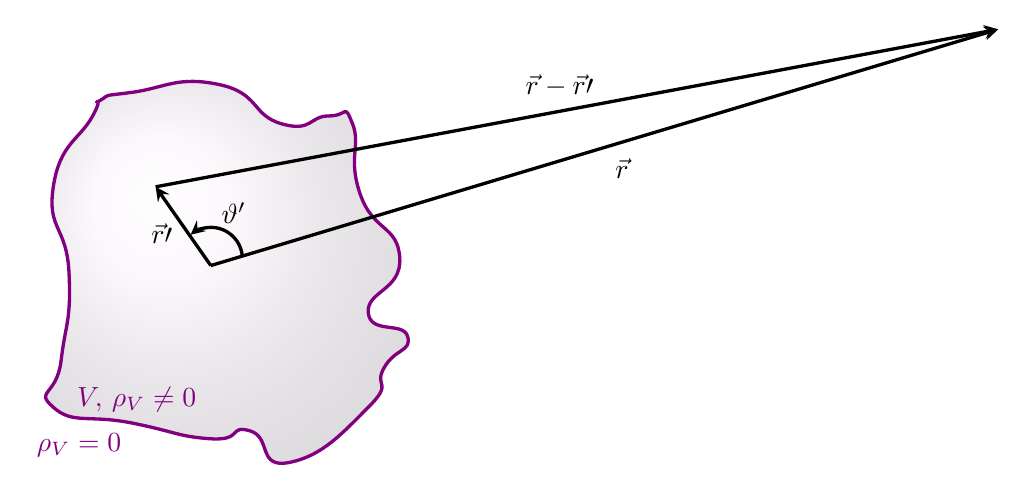
\begin{tikzpicture}[line width = 1.2pt, line join=round,x=1cm,y=1cm,>=stealth]
		% Multipol
		\coordinate (a) at (-1,-2);
		\coordinate (b) at (0,-2.2);
		\coordinate (c) at (0.5,-2.1);
		\coordinate (d) at (1,-2.5);
		\coordinate (e) at (2,-1.8);
		\coordinate (f) at (2.2,-1.3);
		\coordinate (g) at (2.5,-0.9);
		\coordinate (h) at (2,-0.6);
		\coordinate (i) at (2.4,0.1);
		\coordinate (j) at (1.9,0.9);
		\coordinate (k) at (1.8,1.8);
		\coordinate (l) at (1.5,1.9);
		\coordinate (m) at (0.9,1.8);
		\coordinate (n) at (0.1,2.3);
		\coordinate (o) at (-1,2.2);
		\coordinate (p) at (-1.4,2.1);
		\coordinate (q) at (-1.5,1.9);
		\coordinate (r) at (-2,1);
		\coordinate (s) at (-1.8,-0.1);
		\coordinate (t) at (-1.9,-1.2);
		\coordinate (u) at (-2,-1.8);
		\shade[ball color=white!10!violet!20,opacity=0.20] plot [smooth cycle, tension = 1] coordinates {(b) (c) (d) (e) (f) (g) (h) (i) (j) (k) (l) (m) (n) (o) (p) (q) (r) (s) (t) (u) (a)};
		\draw [color=violet] plot [smooth cycle, tension = 1] coordinates {(b) (c) (d) (e) (f) (g) (h) (i) (j) (k) (l) (m) (n) (o) (p) (q) (r) (s) (t) (u) (a)} node [sloped, above] {\ $V,\, \rho_\text{V} \neq 0 $};
		\draw [color=violet] (a) node[anchor=north east] {$ \rho_\text{V} = 0 $};
		% Winkel theta'
		\draw [color=black,->] (10/25,3/25) arc (5:130:10/25);
		\draw [color=black] (0,0.4) node[anchor = south west] {$\vartheta'$};
		% Punkte
		\coordinate (oa) at (10,3);
		\coordinate (ob) at (-0.7,1);
		% Ortsvektor
		\draw [->] (0,0) -- (oa);
		\draw (5,1.5) node[anchor = north west] {$\vec{r} $};
		% Quellvektor
		\draw [->] (0,0) -- (ob);
		\draw (-0.35,0.4) node[anchor = east] {$ \vec{r}\prime  $};
		% Abstandsvektor
		\draw [->,color=black] (ob) -- (oa);
		\draw [color=black] (5,2) node[anchor=south east] {$\vec{r}  - \vec{r}\prime $};
	\end{tikzpicture}
\end{center}
	  Betrachtet wird ein beliebig geformtes räumliches Gebiet mit einer Ladungsverteilung $\neq 0$. Außerhalb des Gebietes gibt es keine Ladung. Interessant ist das Gebiet deutlich außerhalb dieses Giebietes. Mit $\vec{r}'$ wird das Ladungsgebiet durchlaufen (Aufpunkt). $\vec{r}$ ist der Vektor des Beobachtungspunktes. Die Idee ist, dass wenn der Beobachtungspunkt weit genug weg ist, kein wesentlicher Unterschied mehr zwischen $\vec{r}$ und $\vec{r}-\vec{r}'$ besteht. Die Lösung ist z.B. über das Coulomb-Integral ($\nearrow$ \ref{CoulInt}) möglich, in der Regel aber nicht analytisch. Gesucht ist eine analytische Näherungslösung für \(\left| \vec{r}  \right| \gg \left| \vec{r}'  \right| \). Dafür wird zunächst eine (exakte) Entwicklung von $\frac{1}{|\vec{r} -\vec{r}' |}$ benötigt. Aus dem Dreieck in der Skizze folgt mit dem Cosinussatz:
		        \begin{equation*}\begin{split}
				        \left| \vec{r}  - \vec{r}'  \right|^2
				        &= r^2 +  r'^2 - 2 \cdot r \cdot  r' \cdot \cos \vartheta' \\
				        &= r^2 \cdot \left[ 1 + \left(\dfrac{ r'}{r} \right)^2 - 2 \cdot \dfrac{ r'}{r} \cdot
					        \cos \vartheta' \right]
			        \end{split}\end{equation*}
		        \begin{equation*}
			        \left| \vec{r}  - \vec{r}'  \right| = r \cdot \sqrt{1 + \varepsilon} \text{ mit } \varepsilon = \dfrac{ r'}{r} \cdot \left( \dfrac{ r'}{r} - 2 \cdot \cos \vartheta' \right) \quad \left| \vec{r}  \right| \gg \left| \vec{r}'  \right| \to \varepsilon \ll 1
		        \end{equation*}
	  \begin{equation*}\begin{split}
			  \dfrac{1}{\left| \vec{r}  - \vec{r}'  \right|}
			  &= \dfrac{1}{r} \cdot \left( 1 + \varepsilon \right)^{-\frac{1}{2}} = \dfrac{1}{r} \cdot \underbrace{\left( 1 - \dfrac{1}{2} \cdot \varepsilon + \dfrac{3}{8} \cdot \varepsilon^2 - \dfrac{5}{16} \cdot \varepsilon^3 + \dots \right)}_\text{Taylor-Entwicklung}=\frac{1}{r}\left( 1 + \sum_{k=1}^\infty \frac{(-1)^k(2k-1)!}{2^{2k-1}(k-1)!k!} \varepsilon^k\right)
		  \end{split}\end{equation*}
	  Beachte: diese Taylorentwicklung konvergiert nicht gut, lässt man also Terme weg muss \(\left| \vec{r}  \right| \gg \left| \vec{r}'  \right| \) gelten (\(\varepsilon\ll 1\)). Mit eingesetztem \(\varepsilon\) folgt:
	  \begin{equation*}
		  \begin{split}
			  \dfrac{1}{\left| \vec{r}  - \vec{r}'  \right|}
			  = \dfrac{1}{r} \cdot &\left[ 1
				  - \dfrac{1}{2} \cdot \dfrac{ r'}{r} \cdot \left( \dfrac{ r'}{r} - 2 \cdot \cos \vartheta' \right) \right. \\
				  &+ \dfrac{3}{8} \cdot \left( \dfrac{ r'}{r} \right)^2 \cdot \left( \dfrac{ r'}{r} - 2 \cdot \cos \vartheta' \right)^2 \\
				  &\left. - \dfrac{5}{16} \cdot \left( \dfrac{ r'}{r} \right)^3 \cdot \left( \dfrac{ r'}{r} - 2 \cdot \cos \vartheta' \right)^3  + \dots \right]
		  \end{split}
	  \end{equation*}
	  und nach ein wenig Sortierung
	  \begin{equation*}\begin{split}
			  \begin{split}
				  \dfrac{1}{\left| \vec{r}  - \vec{r}'  \right|}
				  = \dfrac{1}{r} \cdot &\left[ \textcolor{red}{1}
					  + \dfrac{ r'}{r} \cdot \textcolor{red}{\cos \vartheta'} \right. \\
					  &+ \left(\dfrac{ r'}{r}\right)^2 \cdot \textcolor{red}{\dfrac{3 \cdot \cos^2 \vartheta' - 1}{2}} \\
					  &+ \left. \left(\dfrac{ r'}{r}\right)^3 \cdot \textcolor{red}{\dfrac{5 \cdot \cos^3 \vartheta' - 3 \cdot \cos \vartheta'}{2}}  + \dots \right]
			  \end{split}
		  \end{split}\end{equation*}
	  Die \textcolor{red}{roten} Terme sind \href{https://de.wikipedia.org/wiki/Legendre-Polynom}{\textbf{Legendre-Polynome}} \(P_{n}(\cos \vartheta')\), somit lässt sich der Ausdruck zu
	  \begin{equation*}
		  \dfrac{1}{\left| \vec{r}  - \vec{r}'  \right|}
		  = \dfrac{1}{r} \cdot \sum\limits_{n=0}^{\infty} \left( \dfrac{ r'}{r} \right)^n \cdot P_n(\cos \vartheta')
	  \end{equation*}
	  verkürzen. Setzt man dies in das Coulomb-Integral ($\nearrow$ \ref{PotR}) ein ergibt sich ($\vec{r}$ muss außerhalb des Quellgebietes liegen, sonst hat man Singularitäten im Integranden):
	  \begin{equation}
		  \boxed{\phi(\vec{r} ) = \frac{1}{4\pi\varepsilon_0} \cdot \sum\limits_{n = 0}^{\infty} \dfrac{1}{r^{n+1}} \cdot \iiint\limits_{V'} ( r')^n \cdot P_\mathrm{n}(\cos \vartheta') \cdot \rho_\text{V}(\vec{r}' ) \dd V'}
	  \end{equation}
	  oder in ausführlicher Schreibweise
	  \begin{equation}\label{multi}
		  \begin{split}
			  \phi(\vec{r} ) = \frac{1}{4\pi\varepsilon_0} \cdot	&\Biggl[ \dfrac{1}{r} \cdot
			  \underbrace{\iiint\limits_{V'} \rho_\text{V}(\vec{r}' ) \dd V'}_{ Q \text{ in Volumen}}
			  + \dfrac{1}{r^2} \cdot \iiint\limits_{V'} \underbrace{ r' \cdot \cos \vartheta'}_{=\dfrac{\vec{r}  \cdot \vec{r}' }{r}} \rho_\text{V} \dd V' \\
			  &+ \dfrac{1}{r^3} \cdot \iiint\limits_{V'} ( r')^2 \cdot \left( \dfrac{3}{2} \cdot \cos \vartheta' - \dfrac{1}{2} \right) \cdot \rho_\text{V}(\vec{r}' ) \dd V' + \dots \Biggr]
		  \end{split}
	  \end{equation}
	  Das Potential des Multipols ergibt sich also aus dem Monopolterm (Gesamtladung)
	  \begin{equation}
		  \phi_\mathrm{M}(\vec{r} )
		  = \frac{1}{4\pi\varepsilon_0} \cdot \dfrac{1}{r} \cdot \iiint\limits_{V'} \rho_\text{V}(\vec{r}' ) \dd V'
		  = \frac{1}{4\pi\varepsilon_0} \cdot \dfrac{ Q}{r}
	  \end{equation}
	  dem Dipolterm
	  \begin{equation}\begin{split}
			  \phi_\mathrm{D}(\vec{r} )
			  &= \frac{1}{4\pi\varepsilon_0} \cdot \dfrac{1}{r^2} \cdot \iiint\limits_{V'}  r' \cdot \cos \vartheta' \cdot \rho_\text{V}(\vec{r}' ) \dd V'\\
			  &= \frac{1}{4\pi\varepsilon_0} \cdot \dfrac{\vec{r} }{r^3} \cdot
			  \underbrace{\iiint\limits_{V'} \vec{r}'  \cdot \rho_\text{V}(\vec{r}' ) \dd V'}_{\vec{p} \text{ von Volumen}}\\
			  &= \frac{1}{4\pi\varepsilon_0} \cdot \dfrac{\vec{r}  \cdot \vec{p}}{r^3}
		  \end{split}\end{equation}
	  dem Quadrupolterm, Oktopolterm und so weiter. Hat man eine endliche Ladung dominiert in der Ferne (Anwendung der Näherung \(\left| \vec{r}  \right| \gg \left| \vec{r}'  \right| \)) der Monopolterm. Hat man keine Ladung, aber ein Dipolmoment, dominiert dieses in der Ferne. Hat man kein Dipolmoment und keine Ladung, aber ein Quadrupolmoment, dominiert dieses in der Ferne. ...\\
	  Durch Simulation mit Python ($\nearrow$ \href{https://github.com/hgkdd/TET/tree/main/programs}{\enquote{programs}}) lässt sich dies auch veranschaulichen. Zoomt man sehr weit raus dominiert die Ladung sofern vorhanden.
\section{Die Poisson-Gleichung und ihre Lösung}\label{poilsg}
	  Das Grundproblem der Elektrostatik ist die Lösung der	Poisson-Gleichung
	  \begin{equation}\begin{split}
			  \Delta \phi(\vec{r} ) = -\frac{1}{\varepsilon_0}
			  \rho_\text{V} (\vec{r} )
		  \end{split}\end{equation}
	  Falls \textbf{keine Randbedingungen} auf Grenzflächen im Endlichen (Potential im unendlichen gegen 0)
	  erfüllt sein müssen kann das Potential bei bekannter
	  Ladungsverteilung aus dem \textbf{Coulomb-Integral} (manchmal auch:
	  Poisson-Integral) berechnet werden ($\nearrow$ \ref{PotR}).\\
	  Im Fall, dass Randbedingungen gegeben sind, ist \textbf{zusätzlich zu} $\rho_\text{V}(\vec{r}' )$ in einem Volumen $V$ \textbf{noch} $\phi$ und/oder $\frac{\partial\phi}{\partial n}=\grad \phi\cdot\vec{n}=-\vec{E} \cdot \vec{n}$ auf Grenz- oder Randflächen in $V$ gegeben $\to$ \textbf{\textit{Randbedingungen}}. $\vec{n}$ ist dabei der ortsabhängige Normalenvektor der betrachteten Grenz- oder Randfläche.
\subsection{Randbedingungen}
		   Um die Poisson-Gleichung in eine Integralgleichung umzuwandeln, wird in der 2. Greenschen Identität ($\nearrow$\ref{green2}) $f\to\phi(\vec{r}' )$ und $g\to \frac{1}{|\vec{r}  - \vec{r}' |}$ (zur Anwendung von $\nearrow$\ref{diraclaplace}) gesetzt (erst reine Mathematik anwenden, dann physikalische Bedeutung geben):
		        \begin{align*}
			        \int\limits_V \left[  \phi(\vec{r}' ) \Delta _{ r'} \frac{1}{|\vec{r}  - \vec{r}' |}  - \frac{1}{|\vec{r}  - \vec{r}' |} \underbrace{\Delta _{ r'}  \phi(\vec{r}' )}_{-\frac{1}{\varepsilon_{0}}\rho_{\text{V}}(\vec{r}')} \right] \dd^3 r' & =  -4\pi \underbrace{\int\limits_V  \phi(\vec{r}' ) \delta^3 (\vec{r}  - \vec{r}' ) \dd^3r'  }_{\phi(\vec{r})}                \\
			                                                                                                                                                                                                                    & + \frac{1}{\varepsilon_0} \int\limits_V \frac{\rho_{\text{V}}(\vec{r}' )}{|\vec{r}  - \vec{r}' |} \dd^3r' \\
			                                                                                                                                                                                                                    & = \oint\limits_{O(V)} \left[\phi\frac{\partial}{\partial n}\frac{1}{|\vec{r}  - \vec{r}' |}
				        - \frac{1}{|\vec{r}  - \vec{r}' |}\frac{\partial\phi}{\partial n} \right] \dd^2r'
		        \end{align*}
		   Somit:
		        \begin{equation}\label{skalarpotGL}\begin{split}
				        \boxed{ \phi(\vec{r} ) = \frac{1}{4\pi\varepsilon_0} \int\limits_V
					        \frac{\rho_\text{V}(\vec{r}' )}{|\vec{r} -\vec{r}' |}
					        \dd^3 r' + \frac{1}{4\pi} \oint\limits_{O(V)} \left[\frac{1}{|\vec{r}  - \vec{r}' |}\frac{\partial\phi}{\partial n} - \phi\frac{\partial}{\partial n}\frac{1}{|\vec{r}  - \vec{r}' |} \right] \dd^2r'}
			        \end{split}\end{equation}
		   Hinweis zur Notation: Im Integral kann man statt $\frac{\partial\phi}{\partial n}$ auch $\frac{\partial\phi}{\partial n'}$ schreiben, um zu verdeutlichen, dass hier die Normalenableitung bezüglich der von $r'$ abhängenden Oberfläche gemeint ist. Die Gleichung ist nicht zur Lösung der Poisson-Gleichung nutzbar (siehe dafür \ref{form}), aber jede Lösung erfüllt sie $\to$ das Problem ist, dass nicht $\phi$ und $\frac{\partial\phi}{\partial n}$ gleichzeitig gegeben sein können, siehe auch \ref{GreenPot}. Dennoch kann man aus ihr die folgenden Schlüsse ziehen:\\
		   Nur Ladungen \textbf{im} Volumen $V$ sowie $\phi$
		        bzw. $\frac{\partial\phi}{\partial n}=\grad \phi\cdot
			        \vec{n}=-\vec{E}\cdot\vec{n}$ bestimmen das Skalarpotential
		        $\phi$ in $V$ (daher die \textbf{\textit{Randbedingungen}}). Ladungen außerhalb von $V$ wirken nur indirekt, sie beeinflussen die Randbedingungen. Wenn keine Ladungen in $V$ vorhanden sind,
		        ist das Skalarpotential vollständig durch die Randwerte
		        festgelegt. Liegen die Ränder von $V$ im Unendlichen ($V$ ist der
		        ganze Raum), verschwindet das Oberflächenintegral, weil
		        der Integrand mit $1/r'^3$ ($\phi\propto 1/r', \partial/\partial n(1/r')\propto 1/r'^2$) abfällt, die Oberfläche aber nur mit $r'^2$ wächst. Es ergibt sich das
		        bereits bekannte Ergebnis für das Skalarpotential im
		        freien Raum nach \ref{PotR}. Die Lösung ist (für das E-Feld) bereits eindeutig bestimmt, wenn
		        für Punkte $\in O(V)$:
		        \begin{enumerate}
			        \item überall $\phi$ gegeben ist: \textbf{Dirichlet
				              Randbedingungen}
			        \item überall $\frac{\partial\phi}{\partial n}=\grad \phi\cdot
				              \vec{n}=-\vec{E}\cdot\vec{n}$ gegeben ist: \textbf{Neumann
				              Randbedingungen}
			        \item für einen Teil der $O_1(V)\subseteq O(V)$ Dirichlet
			              Randbedingungen und für einen anderen (disjunkten!) Teil $O_2(V)\subseteq
				              O(V),\; O_1(V) \mathbin{\dot{\cup}} O_2(V) = O(V)$ Neumannsche Randbedingungen gegeben sind:
			              \textbf{Gemischte Randbedingungen}
		        \end{enumerate}
		  Nun soll gezeigt werden, dass durch die Angabe der Randbedingungen das Problem eindeutig gelöst wird. Seien $\phi_1$ und $\phi_2$ Lösungen der Poisson-Gleichung
		        $\Delta \phi_{1,2}(\vec{r} ) =
			        -\frac{1}{\varepsilon_0}\rho_\text{V}(\vec{r} )$
		        mit gleichen Werten oder gleichen Normalenableitungen auf
		        $O(V)$. Dann ist $\psi=\phi_1-\phi_2$ ($\implies\frac{\partial}{\partial n}\psi=\frac{\partial}{\partial n}\phi_1-\frac{\partial}{\partial n}\phi_2$) Lösung der
		        Laplace-Gleichung (Begründung analog $\nearrow$ \ref{lin}) $\Delta \psi(\vec{r} ) = 0$
		        mit verschwindenden Werten bzw. verschwindender
		        Normalenableitung auf $O(V)$, deshalb wird das Oberflächenintegral in \ref{psigln} $0$. Anwendung der 1. Greenschen Identität ($\nearrow$ \ref{green1}) für den Fall $f=g=\psi$ liefert für beliebige Volumina $V$:
		        \begin{equation}\label{psigln}\begin{split}
				        \int\limits_V \left[ \psi\underbrace{\Delta \psi}_{0} + (\grad
					        \psi\cdot \grad \psi) \right] \dd^3r' &=
				        \oint\limits_{O(V)} \psi\frac{\partial \psi}{\partial n}
				        \dd^2r'\\
				        \implies\int\limits_V (\grad
				        \psi)^2  \dd^3r' = 0 \Rightarrow \grad \psi &=
				        \vec{0} \Rightarrow \psi=\text{const.}
			        \end{split}\end{equation}
		        Die Aussage dieser formalen Herleitung ist, dass die Differenz zweier Lösungen der Poisson-Gleichung ($\phi_1,\phi_2$) mit gleichen (über den kompletten Rand bekannten) Randbedingungen über das Volumen hinweg konstant ist. Nun werden die drei Fälle betrachtet:
		        \begin{enumerate}
		        \item Von $\phi$ ist auf dem Rand der Wert gegeben (\textbf{Dirichlet})
		        \item[] $\Rightarrow$ $\psi=0$ auf dem
		        Rand, also folgt mit $\psi=\const$ in $V$: $
		        {\phi_1=\phi_2}\to
		        \vec{{E}}_{{1}} =\vec{{E}}_{{2}}$
		        \item[] $\Rightarrow$ $\phi$ und $\vec{E}$ sind durch Dirichletsche Bedingungen eindeutig bestimmt
		        \item Von $\phi$ ist auf dem Rand die Normalenableitung gegeben (\textbf{Neumann})
		        \item[]  $\Rightarrow$ $\frac{\partial\psi}{\partial n}=0$ auf dem
		        Rand, also folgt mit $\psi = \text{const.}$ in $V$: $\phi_1=\phi_2 +C\to
		        \vec{{E}}_{{1}}=\vec{{E}}_{{2}}$
		        \item[] $\Rightarrow$ $\phi$ ist bis auf $C$ und $\vec{E}$ ist durch Neummansche Bedingungen eindeutig bestimmt
		        \item Von $\phi$ ist auf dem Rand die stellenweise die Normalenableitung und stellenweise der Wert gegeben (\textbf{gemischt})
		        \item[] $\Rightarrow$ $\psi=0$ (siehe 1.) auf dem
		        Rand, also folgt mit $\psi=\const$ in $V$: $
		        {\phi_1=\phi_2}\to
		        \vec{{E}}_{{1}} =\vec{{E}}_{{2}}$
		        \item[] $\Rightarrow$ $\phi$ und $\vec{E}$ sind durch gemischte Bedingungen eindeutig bestimmt
		        \end{enumerate}
		    Dabei ist zu beachten, dass durch Angabe von $\phi$ \textbf{UND}
		        $\frac{\partial\phi}{\partial n}$ an irgendeinem
		        Punkt von $O(V)$ das Problem bereits
		        \textbf{physikalisch überbestimmt} wäre! \textit{Anschauung:} Allein $\phi$ auf komplettem Rand reicht laut Fall 1. schon aus um $\phi$ im kompletten Volumen eindeutig zu bestimmen!
 \subsection{Formale Lösung} \label{form}
		 Um zwischen Ursache und Wirkung zu vermitteln, werden \textbf{Greensche Funktionen} ($\nearrow$ \ref{greenfkt}) genutzt. Der Ableitungsoperator $\Delta_r$ in der Poisson-Gleichung ($\Delta _r \phi(\vec{r} ) = -\frac{1}{\varepsilon_0} \rho_\text{V}(\vec{r} )$) ist selbstadjungiert (d.h., dass nach \ref{selbstadj} die zugehörigen Greenschen Funktionen symmetrisch sind). Die Bestimmungsgleichung für die Greensche Funktion lautet in diesem Fall $\Delta _rG(\vec{r} ,\vec{r}' ) = -\frac{1}{\varepsilon_0} \delta^3(\vec{r} -\vec{r}' )$ (konstanter Faktor unbedeutend, man kann ihn auch in den Operator hereinziehen). Mit \ref{diraclaplace} kann man \textbf{eine} Greensche Funktion des Laplace-Operators sofort ablesen:
		        \begin{equation}\label{greenLaplace}\begin{split}
				        \boxed{ \Delta _r G(\vec{r} ,\vec{r}' ) = -\frac{1}{\varepsilon_0} \delta^3(\vec{r} -\vec{r}' ) \text{ gilt für } G(\vec{r} ,\vec{r}' ) = \frac{1}{4\pi\varepsilon_0}\frac{1}{|\vec{r} -\vec{r}' |} }
			        \end{split}\end{equation}
		   Zu \textbf{dieser speziellen} Greenschen Funktion kann jedes Element $\Gamma(\vec{r} ,\vec{r}' )$ des Kerns des Laplace-Operators ($\Delta _r \Gamma(\vec{r} ,\vec{r}' ) = 0$) addiert werden, wobei $\Gamma$ eine symmetrische Funktion sein muss (Laplace ist selbstadjungiert):
		        \begin{equation}\label{gammaLaplace}\begin{split}
				        \boxed{G(\vec{r} ,\vec{r}' ) = \frac{1}{4\pi\varepsilon_0}\frac{1}{|\vec{r} -\vec{r}' |} + \Gamma(\vec{r} ,\vec{r}' ) \text{ mit } \Delta _r \Gamma(\vec{r} ,\vec{r}' ) = 0,\quad \Gamma(\vec{r} ,\vec{r}' ) =\Gamma(\vec{r}' ,\vec{r} )}
			        \end{split}\end{equation}
			   Analog der Herleitung von \ref{skalarpotGL} folgt unter Nutzung von der 2. Greenschen Identität (\ref{green2} mit $f\to\phi(\vec{r}' )$ und $g\to G(\vec{r} ,\vec{r}' )$):
			        \begin{equation*}\begin{split}
					        \int\limits_V \left[  \phi(\vec{r}' ) {\Delta _{ r'} G(\vec{r} ,\vec{r}' )}  - G(\vec{r} ,\vec{r}' ) \Delta _{ r'}  \phi(\vec{r}' ) \right] \dd^3 r' &=  -\frac{1}{\varepsilon_0} \int\limits_V  \underbrace{\phi(\vec{r}' ) \delta^3 (\vec{r}  - \vec{r}' )}_{\text{\ref{greenLaplace}+Symmetrie}} \dd^3r' \\
					        &+ \frac{1}{\varepsilon_0} \int\limits_V G(\vec{r} ,\vec{r}' )\rho_\text{V}(\vec{r}' ) \dd^3r'\\
					        &= \oint\limits_{O(V)} \left[ \phi\frac{\partial G(\vec{r} ,\vec{r}' )}{\partial n}
						        - G(\vec{r} ,\vec{r}' )\frac{\partial\phi}{\partial n} \right] \dd^2r'
				        \end{split}\end{equation*}
			   Somit:
			        \begin{equation}\label{GreenPot}\begin{split}
					        \boxed{ \phi(\vec{r} ) = \int\limits_V
						        \rho_\text{V}(\vec{r}' ) G(\vec{r} ,\vec{r}' ) \dd^3 r' + \varepsilon_0 \oint\limits_{O(V)} \left[ G(\vec{r} ,\vec{r}' ) \frac{\partial\phi}{\partial n} - \phi\frac{\partial G(\vec{r} ,\vec{r}' )}{\partial n}\right] \dd^2r'}
				        \end{split}\end{equation}
			   Diese Gleichung gilt für jede beliebige Greensche Funktion, also jede Funktion, die \textbf{im Lösungsvolumen} $\Delta _r G(\vec{r} ,\vec{r}' ) = -\frac{1}{\varepsilon_0} \delta^3(\vec{r} -\vec{r}' )$ erfüllt. Im Freiraum (unendliche Oberfläche) verschwindet das Oberflächenintegral, weil der Integrand $\propto 1/r^3$ und die Fläche $\propto r^2$ wächst. Somit kann $G$ nach \ref{greenLaplace} direkt zur Berechnung des Potentials genutzt werden. Betrachtet man jedoch nicht den gesamten Freiraum, so muss die Greensche Funktion dem Problem angepasst werden, da meistens $G\neq 0$ und $\frac{\partial G}{\partial n}\neq 0$ ist, also kein Term im Oberflächenintegral verschwindet. Die Gleichung gilt zwar weiterhin, aber man wird im Allgemeinen nicht gleichzeitig $\phi$ und $\frac{\partial \phi}{\partial n}$ gegeben haben. Hier kommt die freie Wahl von $\Gamma$ entsprechend \ref{gammaLaplace} ins Spiel. Diese ermöglicht es, $G$ so anzupassen, dass einer der beiden Terme in der Berechnung des Potentials nicht beachtet werden muss und das Problem so auf Basis vom gegebenen $\phi$ oder $\frac{\partial \phi}{\partial n}$ wieder gelöst werden kann.\\
			   Das Volumenintegral ist hierbei die partikuläre Lösung ($\nearrow$ \ref{greenfkt}). Das Oberflächenintegral löst die homogene Gleichung, weil:
			   \begin{align*}
			   	\Delta_r\oint\limits_{O(V)} \left[ G(\vec{r} ,\vec{r}' ) \frac{\partial\phi}{\partial n} - \phi\frac{\partial G(\vec{r} ,\vec{r}' )}{\partial n}\right] \dd^2r' &=\frac{1}{\varepsilon_{0}}\left[\Delta_r\phi(\vec{r} )-\int\limits_V \rho_\text{V}(\vec{r}' ) \Delta_r G(\vec{r} ,\vec{r}' ) \dd^3 r'\right]\\
			   	&=\frac{1}{\varepsilon_{0}}\left[\Delta_r\phi(\vec{r} )-\int\limits_V	\rho_\text{V}(\vec{r}' ) \left(-\frac{1}{\varepsilon_0} \delta^3(\vec{r} -\vec{r}' )\right) \dd^3 r'\right]\\
			   	&=\frac{1}{\varepsilon_{0}}\left[-\frac{1}{\varepsilon_0} \rho_\text{V}(\vec{r} )--\frac{1}{\varepsilon_0}\rho_\text{V}(\vec{r} )\right]=0
			   \end{align*}
  \subsubsection{Dirichlet-Randbedingungen; $\phi$ auf $O(V)$ vorgegeben}
		    Sind Dirichlet-Randbedingungen gegeben, ist es günstig $\Gamma(\vec{r} ,\vec{r}' )$ so zu wählen, dass der Term der Normalenableitung in \ref{GreenPot} verschwindet. Also:
		        \begin{equation}\begin{split}
				        \oint\limits_{O(V)} G(\vec{r} ,\vec{r}' ) \frac{\partial\phi}{\partial n} \dd^2r' = 0
			        \end{split}\end{equation}
		    Ein naheliegender (und häufig verwendeter) Ansatz ist:
		        \begin{equation}\begin{split}
				        G(\vec{r} ,\vec{r}' ) = 0 \text{ für } \vec{r}'  \in O(V)
			        \end{split}\end{equation}
		   Damit gilt:
		        \begin{equation}\begin{split}
				        \boxed{ \phi(\vec{r} ) = \int\limits_V \rho_\text{V}(\vec{r}' ) G(\vec{r} ,\vec{r}' ) \dd^3 r' - \varepsilon_0 \oint\limits_{O(V)}  \phi\frac{\partial G(\vec{r} ,\vec{r}' )}{\partial n} \dd^2r'}
			        \end{split}\end{equation}
		        Beispielsweise kann vom Potential einer Punktladung auf die problemangepasste Greensche Funktion für Dirichlet-RB geschlossen werden. Problemangepasste Greensche Funktion und das Potential von einer Punktladung am Ort $\vec{r}'$ unterscheiden sich nur um die Konstante $Q$, wenn auf dem Rand $\phi=0$ gefordert wird\footnote{Analog 2D: Potential Linienladungsdichte $\leftrightarrow$ Greensche Funktion, 1D: Potential Flächenladungsdichte $\leftrightarrow$ Greensche Funktion}.
  \subsubsection{Neumann-Randbedingungen; $\frac{\partial \phi}{\partial n}$ auf $O(V)$ vorgegeben}
		   Sind Neumann-Randbedingungen gegeben, ist es günstig $\Gamma(\vec{r} ,\vec{r}' )$ so zu wählen, dass der Term des Potentials in \ref{GreenPot} entfällt.
		        \begin{equation}\begin{split}
				        \oint\limits_{O(V)} \phi\frac{\partial G(\vec{r} ,\vec{r}' )}{\partial n} \dd^2r' = 0
			        \end{split}\end{equation}
		    Ein naheliegender Ansatz ist:
		        \begin{equation}\begin{split}
				        \frac{\partial G(\vec{r} ,\vec{r}' )}{\partial n} = 0 \text{ für } \vec{r}'  \in O(V)
			        \end{split}\end{equation}
		   Dieser Ansatz funktioniert \textbf{nicht} (außer $\frac{1}{\varepsilon}\approx 0$ kann genähert werden), weil:
		        \begin{equation}\label{ansNEU}\begin{split}
				        \int\limits_V \Delta _{r'}G(\vec{r} ,\vec{r}' ) \dd^3 r' = -\frac{1}{\varepsilon_0} \int\limits_V \delta^3(\vec{r} -\vec{r}' ) \dd^3 r' &= -\frac{1}{\varepsilon_0}\\
				        \int\limits_V \Delta _{r'}G(\vec{r} ,\vec{r}' ) \dd^3 r' = \oint\limits_{O(V)} \grad _{r'}G(\vec{r} ,\vec{r}' ) \cdot\vec{n}' \dd^2 r' = \oint\limits_{O(V)} \frac{\partial G(\vec{r} ,\vec{r}' )}{\partial n} \dd^2 r'\stackrel{\text{Ansatz}}{=}0&\neq -\frac{1}{\varepsilon_0}
			        \end{split}\end{equation}
		    Ein funktionierender Ansatz ist, $\Gamma(\vec{r} ,\vec{r}' )$ so zu wählen, dass
		        \begin{equation}\begin{split}
				        -\varepsilon_0 \oint\limits_{O(V)} \phi\frac{\partial G(\vec{r} ,\vec{r}' )}{\partial n} \dd^2r' = \phi_0 \text{ mit } \phi_0 = \text{const.}
			        \end{split}\end{equation}
		    Die Konstante geht beim Übergang auf die Feldstärke wieder verloren. Bei Neumann-Bedingungen ist das Potential sowieso nur bis auf eine Konstante bestimmt. Häufig wählt man:
		        \begin{equation}\begin{split}
				        \frac{\partial G(\vec{r} ,\vec{r}' )}{\partial n} = -\frac{1}{\varepsilon_0 S} \text{ für } \vec{r}'  \in O(V), \quad S = \text{ Gesamtberfläche des Volumens}
			        \end{split}\end{equation}
		    damit folgt:
		        \begin{equation}\begin{split}
				        \phi_0 = \frac{1}{S}\oint\limits_{O(V)} \phi(\vec{r}' ) \dd^2r'
			        \end{split}\end{equation}
		    Das ergibt dann:
		        \begin{equation}\begin{split}
				        \boxed{ \phi(\vec{r} ) -\phi_0 = \int\limits_V
					        \rho_\text{V}(\vec{r}' ) G(\vec{r} ,\vec{r}' ) \dd^3 r' + \varepsilon_0 \oint\limits_{O(V)} G(\vec{r} ,\vec{r}' ) \frac{\partial\phi}{\partial n} \dd^2r'}
			        \end{split}\end{equation}
  \subsection{Konkrete Lösungsverfahren}
		   Methoden zur Ermittlung des Potentials sind:
		   \begin{itemize}
		   \item\textbf{Spiegelungsmethode}, \textbf{Bildladungsmethode} ($\nearrow$ \ref{spieg}): Platziere zusätzliche Ladungen \textbf{außerhalb} von $V$, überlagere die Potentiale und leite eine problemangepasste Greensche Funktion ab.
		  \item\textbf{Separation der Variablen} ($\nearrow$ \ref{sep}): Separiere $\phi$ in Teile, die jeweils nur von einer Variablen abhängen und reduziere dadurch ein pDGL auf gDGL Problem (bzw. einfacheres pDGL-Problem).
		  \item \textbf{Orthogonale Funktionensysteme} ($\nearrow$ \ref{elorth}): Entwickle das Potential in eine generische Reihe und passe diese den Randbedingungen an.
		  \end{itemize}
 \subsection{Spiegelladungsmethode}\label{spieg}
 Die Spiegelladungsmethode ist ein Lösungsansatz in der Elektrostatik, bei dem real vorhandene Komponenten durch virtuelle Ladungen ersetzt werden, welche die Randbedingungen replizieren (sie haben nur über die Randbedingungen Einfluss auf das Potential im Lösungsvolumen). Es gilt, dass das elektrische Skalarpotential in einem Volumen eindeutig durch die Ladungsdichte und die Randbedingungen determiniert ist ($\nearrow$ \ref{GreenPot}). Es ist daher möglich, außerhalb des interessierenden Volumens virtuelle Ladungen einzufügen, die die Randbedingungen nachbilden, um eine Struktur zu erhalten, die einfacher zu analysieren ist. Die Methode kann unter anderem genutzt werden, um die Feldstärke oder das Potential einer Anordnung direkt durch Superposition zu erhalten, aber auch um eine Greensche Funktion für eine bestimmte Geometrie zu generieren. Um damit dann \ref{GreenPot} anwenden zu können ist es wünschenswert, dass $G$ (bzw. ein $\Gamma$ des Kerns) Terme mit unbekannten Informationen, also je nach Art der Randbedingung die Normalenableitung oder das Potential, verschwinden lässt. 
 \subsubsection{Grundsätzliches zur Spiegelung an der Ebene}
		  Das Volumenintegral in \ref{GreenPot} ist eine partikuläre Lösung der inhomogenen Poissongleichung, die durch {die Ladungen im Lösungsvolumen} bestimmt wird. Nach der Lösungstheorie linearer Differentialgleichungen ($\nearrow$\ref{lin}) kann hierzu eine beliebige Lösung $\phi_\text{h}$ des homogenen Problems im Lösungsvolumen addiert werden, der entstehende Ausdruck ($\phi=\phi_\text{p}+\phi_\text{h}$) löst die inhomogene Gleichung dann immernoch allgemein. Bei der Spiegelladungsmethode wird $\phi_\text{h}$ durch eine weitere Ladungsdichte außerhalb des Lösungsvolumens erzeugt, sodass die gegebenen Randbedingungen immernoch eingehalten werden. Dadurch, dass die Spiegelladung außerhalb des Lösungsvolumens angeordnet ist, gilt innerhalb des Lösungsvolumens wie gewünscht: $\Delta \phi_\text{h}=0$. Um die eine Greensche Funktion zu generieren, die für die gegebene Anordnung passend ist, muss ein Term $\Gamma$ zu der \textbf{Greenschen Funktion des Freiraums} $G (\vec{r} ,\vec{r}' ) = \frac{1}{4\pi\varepsilon_0} \frac{1}{|\vec{r} -\vec{r}' |}$ hinzuaddiert werden. Dafür kann genutzt werden, dass sich das elektrische Feld einer Punktladung und die Greensche Funktion des Freiraums nur um die multiplikative Konstante $Q$ unterscheiden. Zum Ermitteln der Greenschen Funktion wird also eine Punktladung im Lösungsvolumen betrachtet und eine gleich große Ladung symmetrisch dazu im Zusatzvolumen. Das Vorzeichen dieser Ladung hängt davon ab, ob die Greensche Funktion für Dirichlet- oder Neumann Randbedingungen genutzt werden soll.\\ Der Fall, dass die Spiegelung mit einer Ladung gleichen Vorzeichens erfolgt, macht in der Elektrostatik nur bedingt Sinn. $\varepsilon_0$ ist immer vorhanden. Aber in \ref{spiegdielekt1} (Teilvolumen 1 enthält die Ladung) kommt man mit $\varepsilon_1\gg\varepsilon_2\stackrel{\text{min}}{=}\varepsilon_{0}$ näherungsweise auf eine vorzeichengleiche Spiegelung. Das Teilvolumen 2 wäre dann nach \ref{spiegdielekt2} näherungsweise feldfrei. Analog kann für $\varepsilon_1\ll\varepsilon_2$ näherungsweise vorzeichenverschieden gespiegelt werden. Viel sinnvoller ist die vorzeichengleiche Spiegelung jedoch bei Einströmungen im \textbf{Strömungsfeld}, hier kann $\kappa=0$ nämlich tatsächlich existieren.\\
		   Im Fall von Dirichlet Randbedingungen sollte die Ladung ein unterschiedliches Vorzeichen haben \footnote{Das E-Feld verläuft orthogonal zur Spiegelebene. In der Spiegelebene ist bei dieser Superposition zunächst $\phi=0$, bei Division durch $Q$ wird also $G=0$, sodass der Term mit den Normalenableitungen von $\phi$ in \ref{GreenPot} auf dem Rand verschwindet.}, im Fall von Neumann Randbedingungen das selbe \footnote{Das E-Feld verläuft parallel zur Spiegelebene. In der Spiegelebene ist bei dieser Superposition zunächst $\frac{\partial\phi}{\partial n}\approx0$, bei Division durch $Q$ wird also $\frac{\partial G}{\partial n}\approx0$, sodass der Term mit $\phi$ in \ref{GreenPot} auf dem Rand verschwindet. Dies stellt keinen Widerspruch zu \ref{ansNEU} dar, da $\frac{1}{\varepsilon_1}\approx 0$ (Ausgangspunkt dieser Betrachtungen war, dass $\varepsilon_{1}$ sehr groß ist).}. Durch Superposition der Potentiale dieser Ladungen (das Potential der Bildladung löst im Lösungsvolumen die homogene Gleichung) erhält man das Potential, durch Division mit $Q$ dann die gewünschte Greensche Funktion. Diese kann dann genutzt werden, um in der \textbf{selben} Geometrie das Potential bei anderen $\rho_{\text{V}}$ und auch bei anderen Randbedingungen auszurechnen (sofern diese Randbedingunen physikalisch sinnvoll sind $\to$ z.B. nicht Sinnvoll $\frac{\dd \phi}{\dd n}\neq 0$ für $\varepsilon_1\gg\varepsilon_2$ vorzugeben). Da die so generierte Greensche Funktion auf der Spiegelebene $G=0$ oder $\frac{\partial G}{\partial n}\approx0$ erfüllt, muss der Typ der Randbedingung allerdings konstant bleiben. Man kann aber (theoretisch) ein beliebiges Potential auf dem Rand (in der Spiegelebene) verlangen, während man bei der Berechnung der Greenschen Funktion durch die Annahme zweier gleich großer Ladungen das Potential ($\phi=0$ in Spiegelebene) anders festgesetzt hat.
	  \subsubsection{Spiegelung an ideal leitender geerdeter Ebene}
		  \begin{minipage}[t]{0.5\textwidth}
			  \resizebox{!}{4cm}{\input{res/Ladung_Spiegel}}
		  \end{minipage}
		  \begin{minipage}[t]{0.5\textwidth}
			  \raggedright
			  \resizebox{!}{4cm}{\input{res/gespiegelte_Ladung}}
		  \end{minipage}
		  Das Feldlinienbild gleicht dem eines Dipols ($\nearrow$\ref{Dipol}). Der Teilraum {2} ist feldfrei, da er durch die ideal leitende Ebene geschirmt wird. Damit folgt mit \ref{tanE} unmittelbar, dass die Tangentialkomponente des E-Feldes an der Grenzfläche im Raum 1 gleich 0 ist. Das elektrische Feld steht also senkrecht auf der ideal leitenden Ebene. Damit sich die Tangentialkomponenten kompensieren, muss die Bildladung die selbe (vorzeicheninvertierte) Größe und den selben Abstand zur Ebene haben wie die Originalladung. Auf der ideal leitenden Ebene wird Ladung influenziert, welche durch die Bildladung nachgebildet wird. Kann keine Ladung nachgezogen werden (wie hier über Masse), muss man das Problem anders lösen ($\nearrow$ \ref{bspSpieg}). \\\\
	  \textbf{Berechnung Potential, Feld:}\\
			  Die  Randbedingungen sind: \(E^\text{t}(z=0) = 0\) bzw. \(\phi(z=0) = 0\).
			Die Superposition der skalaren Potentiale lautet:
			        \begin{equation}\label{potSpiegEben}
				        \phi(\vec{r} ) = \phi_1 + \phi_2
				        = \frac{1}{4\pi\varepsilon_0} \cdot \left[ \dfrac{ Q}{\sqrt{\rho^2 + (z - a)^2}} + \dfrac{- Q}{\sqrt{\rho^2 + (z + a)^2}} \right]
			        \end{equation}
			         Da keine Abhängigkeit von \(\varphi\) vorliegt, ergibt sich für das elektrische Feld aus der Gradientenbildung:
			        \begin{equation}
				        \begin{split}
					        \vec{E}(\vec{r} ) = \frac{Q}{4\pi\varepsilon_0} \cdot
					        &\left[ \left( \dfrac{\rho}{\left( \rho^2 + (z - a)^2 \right)^{\frac{3}{2}}} - \dfrac{\rho}{\left( \rho^2 + (z + a)^2 \right)^{\frac{3}{2}}} \right) \cdot \vu{\rho} \right. \\
						        &	 \left. + \left( \dfrac{z - a}{\left( \rho^2 + (z - a)^2 \right)^{\frac{3}{2}}} - \dfrac{z + a}{\left( \rho^2 + (z + a)^2 \right)^{\frac{3}{2}}} \right) \cdot \vu{z} \right]
				        \end{split}
			        \end{equation}
			  Für die Ebene \(z = 0\) gilt demnach
			        \begin{equation}\begin{split}
					        \vec{E}(z=0) &= \frac{Q}{4\pi\varepsilon_0} \cdot \left[ 0 \cdot \vu{\rho} - 2 \cdot \dfrac{a}{\left( \rho^2 + a^2 \right)^{\frac{3}{2}}} \cdot \vu{z} \right] \\
					        &= -\frac{Q}{2\pi\varepsilon_0} \cdot \dfrac{a}{\left( \rho^2 + a^2 \right)^{\frac{3}{2}}} \cdot \vu{z} \\
					        &= E_z \cdot \vu{z} = -E^\text{n} \cdot \vu{z}   \to \text{ Nur eine Normalkomponente}
				        \end{split}\end{equation}
	  \textbf{Berechnung Ladung:}\\
			   Aus der Stetigkeitsbedingung nach \ref{normD} folgt mit der Feldfreiheit des Teilraums 2:  $- \varepsilon_0E^\text{n} = \varepsilon_0E_z = \rho_\text{F}$, also:
			        \begin{equation}
				        \rho_\text{F}(\rho) = -\dfrac{ Q a}{2 \pi  \left( \rho^2 + a^2 \right)^{\frac{3}{2}}}
			        \end{equation}
			  Die Gesamtladung der Fläche ist:
			        \begin{equation}
				        Q_\text{ges. Fläche} = \int\limits_{\varphi'=0}^{2 \pi} \int\limits_{\rho'=0}^{\infty} \rho_\text{F}(\rho') \rho' \dd{}{\rho'} \dd{}{\varphi'} = - Q
			        \end{equation}
			   Die Gesamtladung der Anordnung ist $Q-Q=0$, also gibt es keinen Monopolterm in der Multipolentwicklung. Das Feld gleicht einem reinen Dipol. Zu beachten ist, dass die Gleichungen nur für das Lösungsgebiet gültig sind! Im Zusatzgebiet ist sowieso alles 0 durch die Abschirmung.\\\\
	  \textbf{Greensche Funktion des Halbraums}:\\
			  Aus dem Skalarpotential in \ref{potSpiegEben} kann man $G$ einfach ablesen, da sich das elektrische Potential einer Punktladung und die Greensche Funktion nach \ref{greenLaplace} nur um den konstanten Faktor $Q$ unterscheiden. Eine Punktladung sorgt genau wie die Greensche Funktion für eine $\delta$-Inhomogenität durch Anwendung des Laplace-Operators:
			        \begin{equation}\label{GreenEbene}
				        G(\vec{r} , \vec{r}' ) = \frac{1}{4\pi\varepsilon_0} \cdot \left[
				        \dfrac{1}{|\vec{r}  - \rho' \vu{\rho} - z' \vu{z} |} -
				        \dfrac{1}{|\vec{r}  -\rho' \vu{\rho} + z' \vu{z}|}
				        \right] = 0 \text{ auf } O(V)
			        \end{equation}
			   Damit können durch Anwendung von \ref{GreenPot} auch \textbf{andere Randwertprobleme gleicher Geometrie} (die ideal leitende Ebene muss dort bleiben, wo sie ist) gelöst werden, es gilt:
			        \begin{equation}\begin{split}
					        \frac{\partial G(\vec{r} ,\vec{r}' )}{\partial n} = \frac{1}{4\pi\varepsilon_0} \cdot \left[
						        \dfrac{\vec{r}  - \vec{r}' }{|\vec{r}  - \vec{r}' |^3} +
						        \dfrac{\vec{r}  + \vec{r}' }{|\vec{r}  + \vec{r}' |^3}
						        \right]\cdot\vec{n}
				        \end{split}\end{equation}\\
	  \textbf{Nachrechnen für $\phi(z=0)=\phi_0$}:\\
			  Es wird die selbe Anordnung wie bei der Berechnung der Greenschen Funktion betrachtet, mit der Änderung, dass die ideal leitende Ebene das Potential $\phi_0$ (vorher 0) hat. Die Ladung befindet sich bei $\rho'=0$, $z'=a$, die Greensche Funktion lautet also:
			        \begin{equation}
				        G(\vec{r} , \vec{r}' ) = \frac{1}{4\pi\varepsilon_0} \cdot \left[
					        \dfrac{1}{\sqrt{\rho^2 + (z - a)^2}} +
					        \dfrac{-1}{\sqrt{\rho^2 + (z + a)^2}} \right]
			        \end{equation}
			   Für die Anwendung von \ref{GreenPot} benötigt man die Normalenableitung von $G$ am Ort der Oberfläche, $G$ ist nach \ref{GreenEbene} bei $z'=0$ sowieso 0, der Term der Normalenableitung des Potentials braucht also nicht betrachtet zu werden (Dirichlet-Randbedingungen):
			        \begin{equation}\begin{split}\nonumber
					        \left. \frac{\partial G}{\partial n}\right|_{O(V)} & =\left. \grad G \cdot \vec{n}\right|_{O(V)} = - \left. \frac{\partial G}{\partial z}\right|_{z=0}\\
					        &= - \frac{1}{4\pi\varepsilon_0} \left[  -\frac{1}{2} ( \rho^2 + (z-a)^2 )^{-\frac{3}{2}}(2z-2a) +\frac{1}{2} ( \rho^2 + (z+a)^2 )^{-\frac{3}{2}}(2z+2a) \right]_{z=0}\\
					        &= - \frac{1}{4\pi\varepsilon_0} \left[  \frac{a}{(\rho^2 + a^2 )^{\frac{3}{2}}}  + \frac{a}{(\rho^2 + a^2 )^{\frac{3}{2}}} \right] = - \frac{1}{2\pi\varepsilon_0} \frac{a}{(\rho^2 + a^2 )^{\frac{3}{2}}}
				        \end{split}\end{equation}
			   Einsetzen der Randbedingung $\phi(z=0) = \phi_0$ liefert:
			        $$
				        \phi(\vec{r} ) = \textcolor{green}{\phi_V} + \textcolor{red}{\phi_{O(V)}} = \textcolor{green}{\int\limits_V
					        \rho_\text{V}(\vec{r}' ) G(\vec{r} ,\vec{r}' ) \dd^3 r'} \textcolor{red}{- \varepsilon_0 \oint\limits_{O(V)} \phi_0 \frac{\partial G(\vec{r} ,\vec{r}' )}{\partial n} \dd^2r'}
			        $$
			   Umformung des zweiten Terms:
			        \begin{equation}\begin{split}\nonumber
					        \phi_{O(V)} &= -\varepsilon_0\phi_0 \int\limits_{O(V)} \frac{-1}{2\pi\varepsilon_0} \frac{a}{(\rho^2 + a^2 )^{\frac{3}{2}}} \rho\dd\rho\dd\varphi \\
					        &=  \phi_0 \int\limits_0^\infty  \frac{a\rho}{(\rho^2 + a^2 )^{\frac{3}{2}}} \dd\rho, \quad \zeta = \rho^2+a^2, \quad \dd \zeta = 2\rho\dd \rho \\
					        & = \frac{1}{2} \phi_0 a \int\limits_{a^2}^\infty \frac{1}{\zeta^{\frac{3}{2}}} \dd\zeta =  \frac{1}{2} \phi_0 a  \left[ \frac{-2}{\sqrt{\zeta}}  \right]_{a^2}^{\infty} =  \frac{1}{2} \phi_0 a  \left[ -0 + \frac{2}{a}  \right] \\
					        &=  \phi_0  \frac{a}{a} =  \phi_0
				        \end{split}\end{equation}

			   Wie erwartet ergibt sich das Potential als Summe des Potentials $ \textcolor{green}{\phi_V}$ im Volumen für $\phi=0$ auf der Oberfläche und dem tatsächlichen Potential $\textcolor{red}{\phi_0}$ auf der Oberfläche:
			   \begin{equation}\boxed{\phi(\vec{r} ) = \textcolor{green}{\phi_V} + \textcolor{red}{\phi_0}}\end{equation}
  \subsubsection{Spiegelung an ideal leitender geerdeter Kugel}
	  \begin{center}
		  \input{res/Kugelspiegelung}
	  \end{center}
		  Der Koordinatenursprung wird in den Kugelmittelpunkt gelegt, also folgt mit unbekanntem $\alpha$ und unbekanntem $s_2$ durch Superposition zunächst:
		        $$
			        \phi(\vec{r} ) = \frac{1}{4\pi\varepsilon_0} \left[ \frac{Q}{|r\vu{r}-s_1\vu{r}'|}  - \frac{\alpha Q}{|r\vu{r}-s_2\vu{r}'|}   \right]
		        $$
		   Einsetzen von $\phi(\vec{r}  = R\vu{r})= 0$ (Äquipotentialfläche in der leitenden Ebene wird verlangt):
		        $$
			        \frac{1}{|R\vu{r}-s_1\vu{r}'|}  = \frac{\alpha }{|R\vu{r}-s_2\vu{r}'|}
		        $$
		   Die Bedingung wird erfüllt mit:
		        \begin{equation}
			        \boxed{s_2 = \frac{R^2}{s_1}, \quad \alpha = \frac{R}{s_1}}
		        \end{equation}
	  \textbf{Greensfunktion der Kugel:}\\
			   Mit den gefundenen Bedingungen ($s_1\leftrightarrow r, s_2\leftrightarrow r'$) ergibt sich das Potential $\phi$ bzw. die \textbf{Greensche Funktion der Kugel} mit Radius $R$ (die Geometrie muss gleich bleiben!) $G(\vec{r} ,\vec{r}' ) = \phi/Q$ zu:
			        \begin{equation}\begin{split}
					        G(\vec{r} ,\vec{r}' ) & = \frac{1}{4\pi\varepsilon_0} \left[ \frac{1}{|\vec{r}  - \vec{r}' |}  -  \frac{1}{|\frac{r'}{R}\vec{r}  - \frac{R}{r'}\vec{r}' |} \right] \\
					        & = \frac{1}{4\pi\varepsilon_0} \left[  ( r^2+{r'}^2-2rr'\vu{r}\cdot \vu{r'})^{-\frac{1}{2}}   - \left( \frac{r^2{r'}^2}{R^2}+R^2-2rr'\vu{r}\cdot \vu{r'}  \right)^{-\frac{1}{2}} \right]
				        \end{split}\end{equation}
				Damit ist eine Greensche Funktion gefunden (alle Eigenschaften erfüllt!), die wieder zur Lösung einer ganzen Klasse von Problemen genutzt werden kann (Dirichlet-Randbedingungen, da $G=0$ auf Oberfläche). Die Normalenableitung ist:
			        \begin{equation}\begin{split}
					        \left. \frac{ \partial G(\vec{r} ,\vec{r}' ) }{ \partial n } \right|_{O(V)} =  - \left. \frac{ \partial G(\vec{r} ,\vec{r}' ) }{ \partial r' }\right|_{r'=R}  = - \frac{1}{4\pi\varepsilon_0} \frac{1}{R} \frac{ r^2-R^2 }{ (r^2+R^2-2rR \vu{r}\cdot \vu{r'})^{\frac{3}{2}} }
				        \end{split}\end{equation}
  \subsubsection{Mehrere Spiegelebenen}
		   Der Fall mehrerer (ideal leitender) Ränder führt zu einer Reihe von Spiegelungen.
		   Hierbei müssen auch die \textbf{Spiegelungen der Spiegelung} berücksichtigt werden.
		   Nur bei günstigen Geometrien konvergiert die Reihe. Im folgenden Beispiel sind zwei parallele ideal leitende Ebenen gegeben, zwischen denen eine Volumenladungsdichte eingeschlossen ist. Die schwarzen Bildladungen sind die direkte Spiegelung der Volumenladungsdichte an den beiden Spiegelflächen. Die Bildladungen müssen wieder an den jeweils anderen Flächen gespiegelt werden. Es entstehen die roten Bildladungen. Eine preriodische Fortsetzung der Struktur bis ins unendliche ist nötig.
	  \begin{center}
		  \input{res/unendliche_Spiegelung}
	  \end{center}
  \subsubsection{Formalisierung der Spiegelladungsmethode}
	  \textbf{Problem: Idealer Leiter als Grenzfläche im Volumen}:\\
	 Zunächst soll noch einmal ein idealer geerdeter ($\phi=0$ auf $O(V_2)$) Leiter betrachtet werden. Das Volumen $V_1$ ist das Lösungsvolumen, $V_2$ das Zusatzvolumen (die Leitfähigkeit dort ist unendlich, das Volumen ist feldfrei). $Q_i$ symbolisiert die Volumenladungsdichte ($\rho_{\text{V}}$) im Volumen $V_1$, die Ladungen influenzieren Ladung auf der Oberfläche, folglich ist $\rho_\text{F}\neq0$. Das reale Problem wird durch ein Ersatzproblem repliziert. Der ideale Leiter wird durch das selbe Material wie das Lösungsvolumen ersetzt, es kann dadurch keine influenzierten Oberflächenladungen mehr geben, da dafür ein Leiter benötigt wird. Die Oberflächenladungsdichte wird durch die Bildladungen nachgebildet, welche die Aufgabe haben, weiterhin für $\phi=0$ auf dem Rand zu sorgen. Wenn die Ladung im Außenraum nicht verändert wird und die Randbedingung gleich gehalten wird, dann verändert sich nach \ref{GreenPot} das Potential im Außenraum auch nicht, sodass das Ersatzproblem und das reale Problem für das selbe Potential in $V_1$ sorgen.\\
		  \begin{minipage}{.5\textwidth}
	\centering
	\textbf{reales Problem:}
	\resizebox{.7\textwidth}{!}{
	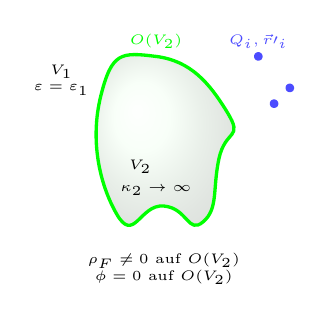
\begin{tikzpicture}[line width = 1.2pt, line join=round,>=stealth]
		\tiny;
		\filldraw [color=blue!70] (2.5,2.5) circle (1pt) node[above] {$Q_i, \vec{r}\prime _i$};
		\filldraw [color=blue!70] (2.9,2.1) circle (1pt);
		\filldraw [color=blue!70] (2.7,1.9) circle (1pt);
		% Ladungsdichte
		\coordinate (a) at (2.1,1.8);
		\coordinate (b) at (2,1.2);
		\coordinate (c) at (1.8,0.4);
		\coordinate (d) at (1.3,0.6);
		\coordinate (e) at (0.7,0.5);
		\coordinate (f) at (0.5,2);
		\coordinate (g) at (1.2,2.5);
		\shade[ball color=white!10!green!20,opacity=0.20] plot [smooth cycle, tension = 1] coordinates {(a) (b) (c) (d) (e) (f) (g)};
		\draw [color=green] plot [smooth cycle, tension = 1] coordinates {(a) (b) (c) (d) (e) (f) (g)} node [sloped, above] {$O(V_2)$};
		\draw (1.3,-0.2) node[align=center] {$\rho_\text{F} \neq 0 $ auf $O(V_2)$\\
			$\phi = 0$ auf $O(V_2)$};
		\draw(1,1.1) node {$V_2$};
		\draw(1.2,0.8) node{$\kappa_2 \to \infty$};
		\draw(0,2.2) node[align=center] {$V_1$\\$\varepsilon=\varepsilon_1$};
	\end{tikzpicture}}
\end{minipage}
\begin{minipage}{.5\textwidth}
	\centering\textbf{Ersatzproblem:}
	\resizebox{.7\textwidth}{!}{
	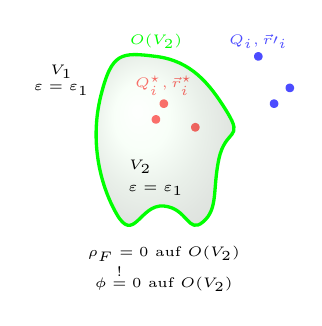
\begin{tikzpicture}[line width = 1.2pt, line join=round,>=stealth]
				\tiny;
		\filldraw [color=blue!70] (2.5,2.5) circle (1pt) node[above] {$Q_i, \vec{r}\prime _i$};
		\filldraw [color=blue!70] (2.9,2.1) circle (1pt);
		\filldraw [color=blue!70] (2.7,1.9) circle (1pt);
		\filldraw [color=red!70] (1.3,1.9) circle (1pt) node[above] {$Q^\star_i, \vec{r} ^\star_i$};
		\filldraw [color=red!70] (1.2,1.7) circle (1pt);
		\filldraw [color=red!70] (1.7,1.6) circle (1pt);
		% Ladungsdichte
		\coordinate (a) at (2.1,1.8);
		\coordinate (b) at (2,1.2);
		\coordinate (c) at (1.8,0.4);
		\coordinate (d) at (1.3,0.6);
		\coordinate (e) at (0.7,0.5);
		\coordinate (f) at (0.5,2);
		\coordinate (g) at (1.2,2.5);
		\shade[ball color=white!10!green!20,opacity=0.20] plot [smooth cycle, tension = 1] coordinates {(a) (b) (c) (d) (e) (f) (g)};
		\draw [color=green] plot [smooth cycle, tension = 1] coordinates {(a) (b) (c) (d) (e) (f) (g)} node [sloped, above] {$O(V_2)$};
		\draw (1.3,-0.2) node[align=center] {$\rho_\text{F} = 0 $ auf $O(V_2)$\\
			$\phi \stackrel{!}{=} 0$ auf $O(V_2)$};
		\draw(1,1.1) node {$V_2$};
		\draw(1.2,0.8) node{$\varepsilon=\varepsilon_1$};
		\draw(0,2.2) node[align=center] {$V_1$\\$\varepsilon=\varepsilon_1$};
	\end{tikzpicture}}
\end{minipage}


		  \textbf{Formale Beschreibung des Ersatzproblems:}
		  \begin{enumerate}
			  \item Es wird eine Abbildung der Quellpunkte auf die Bildpunkte definiert (da später auch $T(T)$ betrachtet wird ist es ungünstig $T: V_1 \cup O(V_2)  \to V_2 \cup O(V_2)$ zu definieren) $T: \IR^3\to\IR^3:\; \vec{r}'  \to \vec{r} ^\star = T( \vec{r}' )$, diese Abbildung sei stetig differenzierbar.
			        Die Bildladungen sollen in $V_2$ liegen, also $T( V_1) \subset V_2$.
			        $O(V_2)$ soll dabei auf sich selbst abgebildet werden, also: $T(\vec{r}  )= \vec{r} $ für $\vec{r}  \in O(V_2)$.
			  \item Es wird eine weitere Funktion definiert, die die Ladungen skaliert. Der Faktor für die Bildladungen sei gegeben durch die Abbildung $\lambda: V_1 \cup O(V_2) \to \mathbb{R}: \vec{r}'  \to \lambda(\vec{r}' )$, welche stetig differenzierbar ist. Ladung auf $O(V_2)$ soll nicht skaliert werden, also gilt $\lambda(\vec{r}' ) = 1$ für $\vec{r}'  \in O(V_2)$.
		  \end{enumerate}
		  Insgesamt wird also $(Q_i, \vec{r}' _i) \to (Q_i^\star, \vec{r} _i^\star) $ abgebildet, mit $Q_i^\star = -\lambda(\vec{r}' _i)\, Q_i$ und $\vec{r} _i^\star = T(\vec{r}' _i)$ (das \enquote{-} ist Konvention).\\
		  	Für das \textbf{Ersatzproblem} kann das elektrische Skalarpotential $\phi(\vec{r} )$ hervorgerufen von den \textbf{Originalladungen} $(Q_i, \vec{r}' _i)$ und den \textbf{Ersatzladungen} $(Q_i^\star, \vec{r} _i^\star)$ direkt mit der \textbf{Greenschen Funktion}
			        \begin{equation}
				        G(\vec{r} ,\vec{r}' ) = \frac{1}{4\pi\varepsilon_1} \frac{1}{\left|\vec{r}  - \vec{r}'  \right|}
			        \end{equation}
			        des homogenen Freiraums $V_2\cup V_1$ berechnet werden, da es sich um ein durchgehendes homogenes Medium ohne Ränder handelt. Es werden hier nur Punktladungen betrachtet, eine kontinuierliche Volumenladungsdichte folgt analog. In $V_2$ ist das Potential real ein anderes als im Ersatzproblem, in $V_1$ ist das Potential das selbe.  Es gilt somit:
			        \begin{eqnarray} \label{PotFormal}
				        \phi(\vec{r} ) & = &\sum_i \left[ Q_i G(\vec{r} ,\vec{r}' _i) + Q_i^\star G(\vec{r} ,\vec{r} _i^\star)\right]\\
				        & = &  \sum_i \left[ Q_i G(\vec{r} ,\vec{r}' _i) -\lambda(\vec{r}' _i) Q_i G(\vec{r} ,T(\vec{r}' _i))\right]\\
				        & = & \sum_i Q_i \left[G(\vec{r} ,\vec{r}' _i) -\lambda(\vec{r}' _i) G(\vec{r} ,T(\vec{r}' _i))\right]
			        \end{eqnarray}
			   Für $\vec{r}  \in O(V_2)$ muss gelten: $\phi(\vec{r} ) = 0$.
			   Für $\vec{r}  \in O(V_2)$ gilt nach der Abbildungsdefinition auch: $\lambda(\vec{r} ) = 1$ und $T(\vec{r} ) = \vec{r} $.\\\\
	  \textbf{Suchen der problemangepassten Greenschen Funktion für das reale Problem:}\\          
			   Auf der Oberfläche von $V_2$ muss das Potential verschwinden (Einhaltung der Randbedingung), also folgt mit \ref{PotFormal}:
			        \begin{equation}
				        \phi(\vec{r} ) =  \sum_i Q_i \left[G(\vec{r} ,\vec{r}' _i) -\lambda(\vec{r}' _i) G(\vec{r} ,T(\vec{r}' _i))\right] \stackrel{!}{=} 0 \text{ für } \vec{r}  \in O(V_2)
			        \end{equation}
			   \textbf{Hinreichend} dafür ist, dass gilt:
			        \begin{equation}\label{umwaelz}
				        \boxed{\lambda(\vec{r}' _i) G(\vec{r} ,T(\vec{r}' _i)) \stackrel{!}{=}  \lambda(\vec{r} ) G(T(\vec{r} ), \vec{r}' _i)}
			        \end{equation}
			   Denn dann gilt auf $O(V_2)$ (weil die Abbildungen $\lambda,T$ auf dem Rand mit diesen Eigenschaften definiert sind):
			        \begin{equation}
				        \lambda(\vec{r}' _i) G(\vec{r} ,T(\vec{r}' _i)) =  \underbrace{\lambda(\vec{r} )}_{=1} G(\underbrace{T(\vec{r} )}_{=\vec{r} },\vec{r}' _i) =  G(\vec{r} ,\vec{r}' _i) \text{ für } \vec{r}  \in O(V_2)
			        \end{equation}
			   Man bezeichnet dies als \textbf{Umwältzen vom Quellpunkt zum Aufpunkt}.
			       Fügt man \ref{umwaelz} und \ref{PotFormal} zusammen folgt:
			        \begin{equation}
				        \phi(\vec{r} ) =  \sum_i Q_i \left[G(\vec{r} ,\vec{r}' _i) -\lambda(\vec{r}' _i) G(\vec{r} ,T(\vec{r}' _i))\right] =\sum_i Q_i \left[G(\vec{r} ,\vec{r}' _i) -\lambda(\vec{r} ) G(T(\vec{r} ),\vec{r}' _i)\right]
			        \end{equation}
			        Dieser Ausdruck ist dann auch Lösung des \textbf{ursprünglichen Problems}, denn für $\vec{r}  \in V_1 \cup O(V_2)$ gehen hier nur die Originalladungen an den Originalorten ein und die Randbedingung ist automatisch erfüllt.
			   Die \textbf{problemangepasste Greensche Funktion} ist damit
			        \begin{equation}\label{problemGreen}
				        \boxed{G^\star(\vec{r} ,\vec{r}' _i) = G(\vec{r} ,\vec{r}' _i) -\lambda(\vec{r} ) G(T(\vec{r} ),\vec{r}' _i)}
			        \end{equation}
			   Das Problem reduziert sich somit auf das Finden der Abbildungen $T$ und $\lambda$. Es reicht dafür (wie vorher) aus, nur eine Punktladung zu betrachten, um die Greensche Funktion für die entsprechende Geometrie zu erhalten.
		    \subsubsection{Beispiele für die formalisierte Spiegelladungsmethode}\label{bspSpieg}
		    \textbf{Spiegelung an einer ideal leitenden Ebene:}\\
		  \begin{center}
		  	
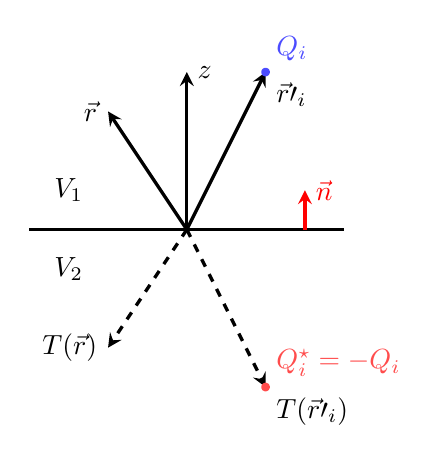
\begin{tikzpicture}[line width = 1.2pt, line join=round,>=stealth]
	\coordinate (O) at (0,0);
	\coordinate (a) at (-2,0);
	\coordinate (b) at (2,0);
	\draw (a) -- (b);
	\draw[color=red, -stealth] (1.5,0) -- (1.5,.5) node[right] {$\vec{n}$};
	\draw[ -stealth] (O) -- (0,2) node[right] {$z$};
	\draw[ -stealth] (O) -- (-1,1.5) node[left] {$\vec{r} $};
	\draw[ dashed, -stealth] (O) -- (-1,-1.5) node[left] {$T(\vec{r} )$};
	\draw[ -stealth] (O) -- (1,2) node[below right] {$\vec{r}\prime _i$};
	\filldraw [color=blue!70] (1,2) circle (1pt) node[above right] {$Q_i$};
	\draw[ dashed, -stealth] (O) -- (1,-2) node[below right] {$T(\vec{r}\prime _i)$};
	\filldraw [color=red!70] (1,-2) circle (1pt) node[above right] {$Q_i^\star=-Q_i$};
	\draw(-1.5,0.5) node {$V_1$};
	\draw(-1.5,-0.5) node {$V_2$};

\end{tikzpicture}
		  \end{center}
		  $V_2$ ist feldfrei. Die Abbildungen $T,\lambda$ sind intuitiv klar, da sich eine gleichgroße Ladung im selben Abstand (in Normalenrichtung) zu der Ebene befinden muss.
		  	\begin{equation}\begin{split}
		  			T:\; &\IR^3\to\IR^3: \; \vec{r}  \to T(\vec{r} ) \\
		  			\Aboxed{&T(\vec{r} ) = \vec{r}  - 2 \vec{n} (\vec{n}\cdot \vec{r} )}\\
		  			\lambda:\; &V_1\cup O(V_2) \to \mathbb{R}: \vec{r}'  \to \lambda(\vec{r}' )\\
		  			\Aboxed{&\lambda(\vec{r}' ) = 1}
		  	\end{split}\end{equation}
		  	 Die Anforderungen an $T$ und $\lambda$ sind offensichtlich erfüllt: Die Bildladungen sind durch Anwendung der Spiegeltransformation in $V_2$ platziert, der Rand $O(V_2)$ wird auf sich selbst abgebildet und  $\lambda(\vec{r}' ) = 1$ auf dem Rand ($\vec{r}'  \in O(V_2)$).	\\	  		  
		  	 Für $\phi = 0$ auf $O(V_2)$ muss \ref{umwaelz} gelten. Das ist erfüllt, da $\lambda$ sowieso 1 ist und die Greensche Funktion des Freiraums $G$ nur vom Abstand seiner Argumente abhängig ist. Grafisch folgt aus der Skizze, dass der Abstand der Argumente in \ref{umwaelz} gleich ist. Um das formal zu zeigen, muss man zunächst nachrechnen, dass $T(T(\vec{r} )) = \vec{r} $ ist (also das Spiegelbild des Spiegelbilds der ursprüngliche Punkt ist):
		  	\begin{equation}\begin{split}
		  			T(T(\vec{r} )) &= T(\vec{r}  - 2 \vec{n} (\vec{n}\cdot \vec{r} ))\\
		  			& = \vec{r}  - 2 \vec{n} (\vec{n}\cdot \vec{r} ) - 2 \vec{n} (\vec{n}\cdot \left\{ \vec{r}  - 2 (\vec{n}\cdot \vec{r} ) \vec{n}  \right\} )  \\
		  			& = \vec{r}  - 2 \vec{n} (\vec{n}\cdot \vec{r} ) - 2 \vec{n} (\vec{n}\cdot \vec{r}  - 2 \vec{n}\cdot \vec{r} )\\
		  			& = \vec{r}  - 2 \vec{n} (\vec{n}\cdot \vec{r} ) - 2 \vec{n} (- \vec{n}\cdot \vec{r} ) = \vec{r}
		  	\end{split}\end{equation}
		  	 Für den Betrag von $\left|T(\vec{r} )\right|$ gilt (weil nur das Vorzeichen der Normalkomponente geändert wird):
		  	\begin{equation}
		  		\left|T(\vec{r} )\right| = \left| \vec{r}  - 2 (\vec{n}\cdot \vec{r} ) \vec{n} \right| = \left| \vec{r}  \right| 
		  	\end{equation}
		  	 Nun kann man \ref{umwaelz}  ($\lambda=1$) nachrechnen:
		  	\begin{equation}\begin{split}
		  			G(\vec{r} , T(\vec{r}' )) &= \frac{1}{4\pi\varepsilon_1} \frac{1}{\left|\vec{r}  -  T(\vec{r}' ) \right|} = \frac{1}{4\pi\varepsilon_1} \frac{1}{\left|T(T(\vec{r} )) - T(\vec{r}' ) \right|} \text{ wegen } T(T(\vec{r} )) = \vec{r} \\
		  			&= \frac{1}{4\pi\varepsilon_1} \frac{1}{\left|T( T(\vec{r} ) - \vec{r}'  )\right|} \text{ weil } T \text{ linear ist}\\
		  			&= \frac{1}{4\pi\varepsilon_1} \frac{1}{\left| T(\vec{r} ) - \vec{r}'  \right|} \text{ weil } \left|T(\vec{r} )\right| = \left| \vec{r}  \right| \\
		  			&= G(T(\vec{r} ), \vec{r}' )
		  	\end{split}\end{equation}
		  	
		  	Damit lautet die problemangepasste Greensche-Funktion:
		  	\begin{equation}\begin{split}
		  			G^\star(\vec{r} ,\vec{r}' _i) & = G(\vec{r} ,\vec{r}' _i) -\lambda(\vec{r} ) G(T(\vec{r} ),\vec{r}' _i)\\
		  			& = G(\vec{r} ,\vec{r}' _i) -\lambda(\vec{r}' _i) G(\vec{r} ,  T(\vec{r}' _i))
		  	\end{split}\end{equation}
		  	
		  	 Mit $\lambda(\vec{r}' ) = 1$ und $T(\vec{r}' ) = \vec{r}'  - 2  \vec{n}  (\vec{n}\cdot \vec{r}' )$ folgt:
		  	\begin{equation}
		  		G^\star(\vec{r} ,\vec{r}' ) = \frac{1}{4\pi\varepsilon_1}  \left(  \frac{1}{\left|\vec{r}  -  \vec{r}'  \right|}  - \frac{1}{\left|\vec{r}  -  \left[ \vec{r}'  - 2 \vec{n} (\vec{n}\cdot \vec{r}' ) \right] \right|}\right)
		  	\end{equation}
		  	 Mit Hilfe der problemangepassten Greenschen Funktion kann das \textbf{Dirichletsche Randwertproblem} in $V_1 \cup O(V_2)$ als \textbf{Freiraumproblem} gelöst werden. Die Randwerte (hier: Skalarpotential ist Null auf dem Rand) werden automatisch erfüllt, solange $\phi=0$ der geforderte Randwert bleibt. Gilt nicht mehr $\phi=0$ müsste man das Oberflächenintegral in \ref{GreenPot} mithilfe von $G^\star$ berechnen, die Normalenableitung des Potentials im Integral verschwindet aber wegen $G^\star=0$ auf dem Rand. Das so gefundene Potential ist \textbf{keine Lösung} in $V_2 \setminus O(V_2)$. Die Berechnung der influenzierten Oberflächenladungsdichte kann mit der (Un-)Stetigkeitsbedingung der Normalkomponente der Dielektrischen Verschiebung erfolgen ($\nearrow$\ref{normD}). Die Gesamtanordnung ist \textbf{ungeladen}, da Oberflächenladung influenziert wird, es gibt also keinen Monopolterm.\\\\
		  \textbf{Spiegelung an der Kante:}\\
		  	 Es werden zwei unendlich ausgedehnte ideal leitfähige Ebenen betrachtet, die durch $\vec{n}_1$ und $\vec{n}_2$ charakterisiert werden. Mit \enquote{Kante} ist die Schnittgerade der beiden Ebenen gemeint, die sich in einem Winkel von $90^\circ$ schneiden sollen. Zunächst wird die Ladung an den beiden Ebenen gespiegelt, dann werden die Spiegelladungen noch einmal gespiegelt. Spiegelt man weiter, landet man wieder auf den gleichen Ladungen, die Anordnung wird also durch 4 Ladungen, jede in einem Raumviertel, charakterisiert. Es ist wichtig, dass Spiegelladungen in $V_1$ verboten sind, weil sonst die Lösung verfälscht würde. Die problemangepasste Greensche-Funktion ist:
		  \begin{align}
		  	G^\star(\vec{r} , \vec{r}' )  =\quad & G (\vec{r} , \vec{r}' )                                                         & \text{Greensche-Funktion des Freiraums} \\
		  	& - G (\vec{r} , T_{\vec{n}_1}(\vec{r}' ))                                        & \text{Spiegelung an Ebene } \vec{n}_1   \nonumber\\
		  	& - G (\vec{r} , T_{\vec{n}_2}(\vec{r}' ))                                        & \text{Spiegelung an Ebene } \vec{n}_2   \nonumber\\
		  	& \underbrace{+}_{(-)( -)}  G (\vec{r} , T_{\vec{n}_2}(T_{\vec{n}_1}(\vec{r}' ))) & \text{Spiegelung der Spiegelung}\nonumber
		  \end{align}
		  Die Ebenen können jeden Winkel $\frac{360^\circ}{n}$ mit $\frac{n}{2}\in\IN$ haben, sodass keine Spiegelladung in $V_1$ selber entsteht. In diesem Fall sieht man genau $n$ Spiegelladungen. Siehe dazu auch das Applet in \enquote{\href{https://bildungsportal.sachsen.de/opal/auth/RepositoryEntry/27455913992/CourseNode/103138906469436/Theoretische\%20Elektrotechnik/Vertiefung/Spiegelladungsmethode}{Spiegelladungsmethode}}.\\\\
		  \textbf{Spiegelung an der ideal leitenden geerdeten Kugel:}
		  \begin{center}
		  	\input{res/SPG3}
		  \end{center}
		  	 Hier kann man die sogenannte \textbf{Kelvin-Transformation} $T$ anwenden. Diese transformiert das innere der Kugel nach außen, das äußere der Kugel nach innen und die Oberfläche bleibt unberührt ($a$ ist der Kugelradius). Die Transformationsgleichung lautet ($\lambda$ ist daraus abgeleitet):
		  	\begin{equation}\label{kelvin}\begin{split}
		  			T & :  \mathbb{R}^3 \to \mathbb{R}^3 : \vec{r}'  \to T(\vec{r}' ) = \frac{a^2}{\left| \vec{r}' \right|^2} \vec{r}'  = a \frac{a}{ r'} \vu{ r'}\\
		  			\lambda & :  \mathbb{R}^3 \to \mathbb{R} : \vec{r}'  \to \lambda(\vec{r}' ) = \frac{a}{\left| \vec{r}' \right|}
		  	\end{split}\end{equation}
		  	 Für $\vec{r}'  \in O(V_2)$ gilt somit: $T(\vec{r}' ) = \vec{r}' $. Außerdem gilt: $T(T(\vec{r}' )) = T(a \frac{a}{{\vec{r}'} } \vu{{\vec{r}' }})=  a \frac{a}{a \frac{a}{\vec{r}' }} \vu{{\vec{r}' }} = \vec{r}' $. Weiterhin folgt aus \ref{kelvin} die Regel der \textbf{reziproken Radien}:
		  	\begin{equation}
		  		\boxed{\left| \vec{r}'  \right| \left| T(\vec{r}' ) \right| = a^2}
		  	\end{equation}
		  	 Die grundlegenden Bedingungen an die Transformation (also die Eigenschaften von $T$ und $\lambda$) sind erfüllt. Die Hinreichende Bedingung für $\phi = 0$ auf $O(V_2)$ nach \ref{umwaelz} muss noch gezeigt werden. Zunächst ist:
		  	\begin{equation}\label{eigKelvin}\begin{split}
		  			\left| T(\vec{r} ) - \vec{r}'   \right|^2 & = \left| \frac{a^2}{\left| \vec{r} \right|^2} \vec{r}  - \vec{r}'  \right|^2 = \frac{a^4}{\left| \vec{r} \right|^2} - \frac{2a^2}{\left| \vec{r} \right|^2} \vec{r}  \cdot \vec{r}'  + \left| \vec{r}' \right|^2 \\
		  			& = \frac{\left| \vec{r}' \right|^2}{\left| \vec{r} \right|^2} \left[  \frac{a^4}{\left| \vec{r}' \right|^2} - \frac{2a^2}{\left| \vec{r}' \right|^2} \vec{r}  \cdot \vec{r}'  + \left| \vec{r} \right|^2 \right] = \frac{\left| \vec{r}' \right|^2}{\left| \vec{r} \right|^2} \left| \vec{r}  - \frac{a^2}{\left| \vec{r}' \right|^2} \vec{r}' \right|^2\\
		  			& = \frac{\left| \vec{r}' \right|^2}{\left| \vec{r} \right|^2} \left| \vec{r}    - T(\vec{r}' ) \right|^2
		  	\end{split}\end{equation}
			$G^\star$ ist nun berechenbar mit \ref{problemGreen}, sofern \ref{umwaelz} gilt:
		  	\begin{equation}\begin{split}
		  			\lambda(\vec{r}' ) G(\vec{r} , T(\vec{r}' )) &= \frac{a}{\left| \vec{r}' \right|} \frac{1}{4\pi\varepsilon_1}\frac{1}{\left| \vec{r}    - T(\vec{r}' ) \right|} = \frac{a}{\left| \vec{r}' \right|} \frac{1}{4\pi\varepsilon_1} \frac{\left| \vec{r}' \right|}{\left| \vec{r} \right|} \frac{1}{\left|  T(\vec{r} ) - \vec{r}'  \right|} \\
		  			&= \frac{a}{\left| \vec{r} \right|} \frac{1}{4\pi\varepsilon_1} \frac{\left| \vec{r}' \right|}{\left| \vec{r}' \right|} \frac{1}{\left|  T(\vec{r} ) - \vec{r}'  \right|} = \lambda(\vec{r} ) G(T(\vec{r} ), \vec{r}' )
		  	\end{split}\end{equation}
		  \textbf{Spiegelung an der ideal leitenden isolierten Kugel:}\\
		  	 Bisher wurde eine \textbf{geerdete Kugel} betrachtet, beim Einbringen der Punktladung änderte sich dort die Ladung der Kugel durch elektrostatische Influenz (Gesamtladung der Anordnung war 0). Damit die Kugel Ladung ziehen kann, muss diese geerdet sein. Bei der isolierten Kugel bleibt die Gesamtladung der Kugel beim Einbringen der Punktladung unverändert (z.B. vorher Null $\to$ nachher Null). Die Bildladung $Q^\star = -\lambda(\vec{r}' ) Q$ verändert aber die Ladung im Volumen $V_2$. Um dies zu kompensieren, kann man zusätzlich eine Ladung im Zentrum der Kugel platzieren. Die Kugeloberfläche ist eine Äquipotentialfläche im Feld dieser Ladung, auf der Kugeloberfläche kommt es durch diese Ladung also nur zu einer Potentialänderung um eine Konstante.
		  	 Die zusätzliche Ladung muss die Größe $-Q^\star$ haben, um das $Q^\star$ von der Spiegelung zu kompensieren, die Gesamtladung der Anordnung ist also im realen und im angepassten Problem $Q$. Die problemangepasste Greensche Funktion lautet ($\nearrow$\ref{kelvin}):
		  	\begin{equation}\begin{split}
		  			G^\star(\vec{r} , \vec{r}' ) & =  G(\vec{r} , \vec{r}' ) - \lambda(\vec{r}' ) G(\vec{r} , T(\vec{r}' )) + \lambda(\vec{r}' ) G(\vec{r} , \vec{0}) \\
		  			& = G(\vec{r} , \vec{r}' ) - \frac{a}{\abs{\vec{r}' }} \left( G\left(\vec{r} , \frac{a^2}{\abs{\vec{r}' }^2} \vec{r}' \right) - G(\vec{r} , \vec{0}) \right) \\
		  			& = \frac{1}{4\pi\varepsilon_1} \left[ \frac{1}{\abs{\vec{r}  - \vec{r}' }} - \frac{a}{\abs{\vec{r}' }} \left( \frac{1}{\abs{\vec{r} - \frac{a^2}{\abs{\vec{r}' }^2} \vec{r}' }} - \frac{1}{ \abs{\vec{r} }} \right) \right]\\
		  			& = \frac{1}{4\pi\varepsilon_1} \left[
		  			\frac{1}{\abs{\vec{r}  - \vec{r}' }}
		  			- \frac{a}{\abs{\vec{r} }} \frac{1}{\abs{\frac{a^2}{\abs{\vec{r} }^2} \vec{r}  - \vec{r}' }}
		  			+\frac{a}{\abs{\vec{r}' }} \frac{1}{ \abs{\vec{r} }}
		  			\right]
		  	\end{split}\end{equation}
	  	Diese ist (auch wenn dies nicht offensichtlich ist) symmetrisch, denn:
	  	\begin{equation*}\begin{split}
	  			G^\star(\vec{r} , \vec{r}' ) & \stackrel{!}{=} G^\star(\vec{r}' , \vec{r} )\\
	  			\cancel{G(\vec{r} , \vec{r}' )} - \lambda(\vec{r}' ) G(\vec{r} , T(\vec{r}' )) + \lambda(\vec{r}' ) G(\vec{r} , \vec{0}) &=\cancel{G(\vec{r}' , \vec{r} )} - \lambda(\vec{r} ) G(\vec{r}' , T(\vec{r} )) + \lambda(\vec{r} ) G(\vec{r}' , \vec{0}) \quad |\, \text{\ref{greenLaplace}} \\
	  			- \lambda(\vec{r}' ) G(\vec{r} , T(\vec{r}' )) + \cancel{\frac{a}{\abs{\vec{r}' }} \frac{C}{|\vec{r}|}} &=  - \lambda(\vec{r} ) G(\vec{r}' , T(\vec{r} )) + \cancel{ \frac{a}{\abs{\vec{r} }} \frac{C}{|\vec{r}'|}} \quad |\,  \text{\ref{umwaelz}\&\ref{greenLaplace}}\\
	  			0&=0
	  	\end{split}\end{equation*}
		  	 Auf der Oberfläche der Kugel kompensieren sich die ersten beiden Beiträge (bei der geerdeten Kugel wäre $G=0$ auf der Oberfläche, es bleibt nur noch der Beitrag Zusatzladung übrig):
		  	\begin{equation}
		  		\left. G^\star(\vec{r} , \vec{r}' )\right|_{\abs{\vec{r} }=a} = \frac{1}{4\pi\varepsilon_1} \frac{1}{\abs{\vec{r}' }} = G(0,\vec{r}' ) \to  \text{ konstant auf } O(V_2)
		  	\end{equation}
		  	Das Potential auf der Oberfläche ist:
		  	\begin{equation}
		  		\left. \phi(\vec{r} )\right|_{\abs{\vec{r} }=a} = \frac{1}{4\pi\varepsilon_1} \frac{Q}{\abs{\vec{r}' }}
		  	\end{equation}
		  	Dies entspricht dem Potential, welches die ursprüngliche Ladung $Q$ (welche sich in der Entfernung $\abs{\vec{r}' }$ zum Ursprung der Kugel befindet) im Ursprung der Kugel hervorrufen würde, wenn die Kugel nicht vorhanden wäre.\\\\
		  \textbf{Spiegelung einer Linienladung am geerdeten Zylinder:}\\
		  	  	 Es wird eine Linienladung vor einem geerdetem und ideal leitfähigem Zylinder betrachtet. Beide sind $z$-gerichtet.
		  	 Zunächst wird die \textbf{Greensche Funktion des Freiraums} für diese Geometrie benötigt. Die Anwendung von \ref{greenLaplace} führt aufgrund der unendlich ausgedehnten Linienladung zu nicht sinnvollen Ergebnissen ($\phi=\infty\forall\rho$). Deshalb wird zunächst eine Linienladung im Freiraum betrachtet.
		  		  \begin{center}
		  	\tdplotsetmaincoords{60}{110}
\begin{tikzpicture}[scale=3, tdplot_main_coords]
	\coordinate (O) at (0,0,0);
	\draw[thick,->] (0,0,0) -- (1,0,0) node[anchor=north east]{$x$};
	\draw[thick,->] (0,0,0) -- (0,1,0) node[anchor=north west]{$y$};
	\draw[thick,->] (0,0,0) -- (0,0,1) node[anchor=east]{$z$};
	\tdplotsetcoord{P}{1}{30}{60}
	\draw plot [mark=*, mark size=0.2] (P) node [above] {\scriptsize$\vec{r} =(\rho,\varphi,z)$};
	\draw[thick, ->] (O) -- (P);
	\draw[dashed, color=black] (O) -- (Pxy) node [below right] {$\rho$};
	\draw[dashed, color=black] (Pxy) -- (P) node [below right] {$z$};
	\tdplotdrawarc{(O)}{0.2}{0}{60}{anchor=north}{$\varphi$}
	% \draw[dashed, color=black] (P) -- (Pz) node [below left] {$z$};
	\draw[thick,color=red, dashed] (0,0,1.2) -- (0,0,-0.6) node[anchor=north] {$\rho_L$};
	\draw (0,-0.2,0.1) node{$V_1,\, \varepsilon_1$};
\end{tikzpicture}
		  \end{center}
		  	 Für das Skalarpotential gilt (z.B. über \ref{gauss} in Integralform herleitbar):
		  	\begin{equation}
		  		\phi(\vec{r} ) = -\frac{\rho_L}{2\pi\varepsilon_1} \ln\left(\frac{\rho}{\rho_B} \right)
		  	\end{equation}
		  	 Dabei bezeichnet $\rho_B$ einen willkürlichen Bezugsabstand, bei dem gilt: $\phi(\vec{r} =(\rho_B,\varphi,z)) = 0$. $\phi$ ist nur von $\rho$ abhängig. Wegen der Translationsinvarianz (bzgl. $z,\varphi$) ist eine Betrachtung in der Ebene $z=0$ ausreichend. Für Ortsvektoren in dieser Ebene gilt:  $\vec{r} \cdot \vec{e_z} = 0$. Damit gilt \textbf{in der $z=0$-Ebene}: $\phi(\vec{r} ) = -\frac{\rho_L}{2\pi\varepsilon_1} \ln\left(\frac{\left|\vec{r} \right|}{\rho_B} \right)$. Für eine um $\vec{r}' $ verschobene Linienladung gilt (auch in Ebene $z=0$!):
		  	\begin{equation}
		  		\boxed{\phi(\vec{r} ) = -\frac{\rho_L}{2\pi\varepsilon_1} \ln\left(\frac{\left|\vec{r} -\vec{r}' \right|}{\rho_B} \right)} \text{ mit }  \vec{r}'\cdot \vec{e_z} = \vec{r}\cdot \vec{e_z}  = 0
		  	\end{equation}
		  	Wegen der Translationsinvarianz der Anordnung ist es egal, ob man einen 2D oder 3D-Laplace anwendet. Hier wird der 2D-Laplace genutzt (Greensfunktion von 3D-Laplace führte auf Probleme). Die Greensche Funktion ist also eine Funktion, die $\Delta G_2(\vec{r},\vec{r}') =-\frac{1}{\varepsilon_{0}}\delta (x-x')\delta(y-y')$ erfüllt  (für Translationsinvarianzen in andere Koordinatenrichtungen analog). Es folgt damit im Freiraum $\phi(\vec{r})=\iint\limits_A G_2(\vec{r},\vec{r}') \rho_{\text{V}} \dd A$. Die \textbf{Greensche Funktion des 2D-Freiraums} $G_2$ (eingebettet in den 3D-Raum) folgt sofort aus der Lösung für das Potential. Es lässt sich zeigen, dass die 3D-Greensche Funktion für Probleme, die unabhängig von einer Koordinatenrichtung (hier: $z$) sind, die Folgende ist:
		  	\begin{equation}
		  		\boxed{G_2(\vec{r} , \vec{r}' )= -\frac{1}{2\pi\varepsilon_1} \ln\left(\frac{\left|\vec{r} -\vec{r}' \right|}{\rho_B} \right) }
		  	\end{equation}
		  Nun wird die Linienladung vor einem ideal leitfähigen geerdeten Zylinder betrachtet:
		  \begin{center}
		  	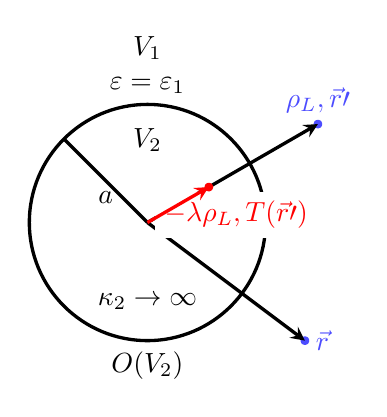
\begin{tikzpicture}[line width = 1.2pt, line join=round,>=stealth]
	\filldraw [color=blue!70] (30:2.5) circle (1pt) node[above] {$\rho_L, \vec{r}\prime $};
	\filldraw [color=blue!70] (2,-1.5) circle (1pt) node[right] {$\vec{r} $};
	\draw [-stealth] (0,0) -- (30:2.5);
	\draw [-stealth] (0,0) -- (2,-1.5);
	\draw (0,0) circle (1.5);
	\draw (0,0) -- (135:1.5);
	\draw (135:0.75 ) node[below] {$a$};

	\draw (0,-1.5) node [below] {$O(V_2)$};
	\draw(0,1.05) node {$V_2$};
	\draw(0,-1) node{$\kappa_2 \to \infty$};
	\draw(0,2.0) node[align=center] {$V_1$\\$\varepsilon=\varepsilon_1$};
	\draw [color=red] (20:1.2) node[below, fill=white] {$-\lambda \rho_L, T(\vec{r}\prime )$};

	\draw [-stealth,color=red] (0,0) -- (30:0.9);
	\filldraw [color=red] (30:0.9) circle (1pt);
\end{tikzpicture}
		  \end{center}
Wegen der Analogie \enquote{Punktladung vor Kugel $\leftrightarrow$ Linienladung vor Zylinder} ist es naheliegend, wieder die \textbf{Kelvin-Transformation}  ($\nearrow$\ref{kelvin}) zu probieren. Für das Potential gilt dann ($\lambda$ ist hier noch unbekannt, nur $T$ ist die Kelvin-Transformation):
		  	\begin{equation}\begin{split}
		  			\phi(a\vec{e_\rho}) & = -\frac{1}{2\pi\varepsilon_1}  \rho_L\left[\ln\left(\frac{\rho - a}{\rho_B} \right) -\lambda \ln\left(\frac{a - T(a\vec{e_\rho})}{\rho_B} \right)  \right] \stackrel{!}{=} 0 \\
		  			& \ln\left(\rho - a \right) -\lambda \ln(a - T(a\vec{e_\rho})) \stackrel{!}{=} 0 \\
		  			& \ln\left(\rho - a \right) -\lambda \ln(a - \frac{a^2}{\rho^2}\rho)) \stackrel{!}{=} 0 \\
		  			& \rho - a \stackrel{!}{=}  \left( a - \frac{a^2}{\rho}\right)^\lambda
		  	\end{split}\end{equation}
		  	 Es gibt also kein $\lambda$, das $\phi = 0$ auf der Oberfläche erzeugt und somit kein $\lambda$, das zusammen mit der Kelvin-Transformation das gewünschte Potential auf der Oberfläche des Zylinders erzeugt. Trotzdem wird $\lambda(\vec{r} )=1$ gesetzt und weiter mit der Kelvin-Transformation gemacht.
		  	 Für diese Transformation wurde \ref{eigKelvin} gezeigt, also folgt:
		  	\begin{equation}\begin{split}
		  			G_2(\vec{r} , T(\vec{r}' )) & = -\frac{1}{2\pi\varepsilon_1} \ln\left(\frac{\left|\vec{r}  - T(\vec{r}' )\right|  }{\rho_B} \right)  = -\frac{1}{2\pi\varepsilon_1} \ln\left(\frac{\left|T(\vec{r} ) - \vec{r}' \right|  \left| \vec{r} \right| }{\rho_B \left| \vec{r}' \right|} \right) \\
		  			&= -\frac{1}{2\pi\varepsilon_1} \left[ \ln\left(\frac{\left|T(\vec{r} ) - \vec{r}' \right| }{\rho_B } \right) + \ln\left(\frac{ \left| \vec{r} \right| }{\rho_B } \right) - \ln\left(\frac{ \left| \vec{r}' \right| }{\rho_B } \right)  \right]\\
		  			&= G_2(T(\vec{r} ), \vec{r}' ) + G_2(\vec{r} , \vec{0}) - G_2(0, \vec{r}' )
		  	\end{split}\end{equation}
		  	 Damit folgt für das Potential:
		  	\begin{equation}\begin{split}
		  			\phi(\vec{r} ) & = \rho_L G_2(\vec{r} , \vec{r}' ) -\rho_L G_2(\vec{r} , T(\vec{r}' )) \\
		  			&= \rho_L \left[ G_2(\vec{r} , \vec{r}' ) - G_2(T(\vec{r} ), \vec{r}' ) - G_2(\vec{r} , \vec{0}) + G_2(0, \vec{r}' )\right]
		  	\end{split}\end{equation}
		  	 Wegen $T(\vec{r} )=\vec{r} $ für $\vec{r}  =a\vec{e_\rho} $ kompensieren sich die ersten beiden Terme auf der Oberfläche:
		  	\begin{equation}
		  		\left.\phi(\vec{r} )\right|_{\vec{r}  =a\vec{e_\rho}} = \rho_L \left[ - G_2(a\vec{e_\rho}, \vec{0}) + G_2(0, \vec{r}' )\right] = \frac{\rho_L}{2\pi\varepsilon_1} \ln\left(\frac{a}{\abs{\vec{r}' }} \right)
		  	\end{equation}
		  	 Vergleich mit Potential einer Linienladung auf der $z$-Achse liefert:
		  	\begin{equation}
		  		\phi(\vec{r} ) = -\frac{\rho_L}{2\pi\varepsilon_1} \ln\left(\frac{\rho}{\rho_B} \right) \rightarrow \left.\phi(\vec{r} )\right|_{\vec{r}  =a\vec{e_\rho}} = -\frac{\rho_L}{2\pi\varepsilon_1} \ln\left(\frac{a}{\rho_B} \right)
		  	\end{equation}
		  	 Offenbar lässt sich $\phi =0$ auf der Zylinderoberfläche durch eine zusätzliche Linenladung auf der $z$-Achse erreichen (wie bei der isolierten Kugel, $\rho_B$ ist beliebig). Mit diesem Zusatz funktioniert hier also die Kelvin-Transformation mit $\lambda = 1$. Die Problemangepasste Greensche Funktion ist gefunden:
		  	\begin{equation}
		  		G^\star (\vec{r} , \vec{r}' ) = G_2(\vec{r} , \vec{r}' ) - G_2(\vec{r} , \frac{a^2}{(\rho')^2}\vec{r}'  )+ \left.G_2(\vec{r} , \vec{0})\right|_{\rho_B = \abs{\vec{r}' }}
		  	\end{equation}
		  \subsubsection{Dielektrische Spiegelung}
		  	 Betrachtet wird Volumen $V_2, \varepsilon_2$ eingebettet in ein Volumen $V_1,\varepsilon_1$. Die Ladungen $(Q_i, \vec{r}' _i)$ in $V_1$ sind vorgegeben (kontinuierliche Dichte analog). Gesucht ist die Lösung in $V_1$ \textbf{und} $V_2$. Die Lösungsidee ist:
		  	\begin{itemize}
		  		\item Für die Berechnung im umgebenden Volumen $V_1$ werden Bildladungen $(Q_i^\star, \vec{r} _i^\star)$ in $V_2$ als Ersatz für das eingebettete Material eingesetzt. In $V_2$ gilt hierfür auch $\varepsilon = \varepsilon_1$.
		  		\item Für die Berechnung im eingebetteten Volumen $V_2$ werden Bildladungen $(Q_i^{\star\star}, \vec{r} _i^{\star\star})$ in $V_1$ als Ersatz für das umgebende Material eingesetzt. In $V_1$ gilt hierfür auch $\varepsilon = \varepsilon_2$.
		  		\item Es soll versucht werden, $\vec{r} _i^{\star\star} = \vec{r}' _i$ zu setzen, also faktisch \enquote{nur} eine Veränderung der ursprünglichen Ladungen zu erzielen und keine externen Ladungen an neuen Positionen hinzuzufügen.
		  	\end{itemize}
		  \begin{minipage}{.33\textwidth}
	\centering
	\textbf{reales Problem:}
	\resizebox{!}{.7\textwidth}{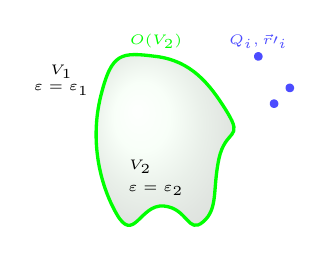
\begin{tikzpicture}[line width = 1.2pt, line join=round,>=stealth]
			\tiny;
		\filldraw [color=blue!70] (2.5,2.5) circle (1pt) node[above] {$Q_i, \vec{r}\prime _i$};
		\filldraw [color=blue!70] (2.9,2.1) circle (1pt);
		\filldraw [color=blue!70] (2.7,1.9) circle (1pt);
		% Ladungsdichte
		\coordinate (a) at (2.1,1.8);
		\coordinate (b) at (2,1.2);
		\coordinate (c) at (1.8,0.4);
		\coordinate (d) at (1.3,0.6);
		\coordinate (e) at (0.7,0.5);
		\coordinate (f) at (0.5,2);
		\coordinate (g) at (1.2,2.5);
		\shade[ball color=white!10!green!20,opacity=0.20] plot [smooth cycle, tension = 1] coordinates {(a) (b) (c) (d) (e) (f) (g)};
		\draw [color=green] plot [smooth cycle, tension = 1] coordinates {(a) (b) (c) (d) (e) (f) (g)} node [sloped, above] {$O(V_2)$};
		\draw(1,1.1) node {$V_2$};
		\draw(1.2,0.8) node{$\varepsilon=\varepsilon_2$};
		\draw(0,2.2) node[align=center] {$V_1$\\$\varepsilon=\varepsilon_1$};
	\end{tikzpicture}}
\end{minipage}
\begin{minipage}{.33\textwidth}
	\centering
	\textbf{Berechnung in} $V_1$:
	\resizebox{!}{.7\textwidth}{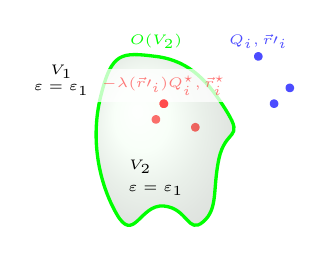
\begin{tikzpicture}[line width = 1.2pt, line join=round,>=stealth]
						\tiny;
		\filldraw [color=blue!70] (2.5,2.5) circle (1pt) node[above] {$Q_i, \vec{r}\prime _i$};
		\filldraw [color=blue!70] (2.9,2.1) circle (1pt);
		\filldraw [color=blue!70] (2.7,1.9) circle (1pt);
		\filldraw [color=red!70] (1.2,1.7) circle (1pt);
		\filldraw [color=red!70] (1.7,1.6) circle (1pt);
		% Ladungsdichte
		\coordinate (a) at (2.1,1.8);
		\coordinate (b) at (2,1.2);
		\coordinate (c) at (1.8,0.4);
		\coordinate (d) at (1.3,0.6);
		\coordinate (e) at (0.7,0.5);
		\coordinate (f) at (0.5,2);
		\coordinate (g) at (1.2,2.5);
		\shade[ball color=white!10!green!20,opacity=0.20] plot [smooth cycle, tension = 1] coordinates {(a) (b) (c) (d) (e) (f) (g)};
		\draw [color=green] plot [smooth cycle, tension = 1] coordinates {(a) (b) (c) (d) (e) (f) (g)} node [sloped, above] {$O(V_2)$};
		\draw(1,1.1) node {$V_2$};
		\draw(1.2,0.8) node{$\varepsilon=\varepsilon_1$};
		\draw(0,2.2) node[align=center] {$V_1$\\$\varepsilon=\varepsilon_1$};
		\filldraw [color=red!70] (1.3,1.9) circle (1pt) node[rectangle,fill=white,above,nearly opaque] {$-\lambda(\vec{r}\prime _i) Q^\star_i, \vec{r} ^\star_i$};
		\filldraw [color=red!70] (1.3,1.9) circle (1pt) ;
	\end{tikzpicture}}
\end{minipage}
\begin{minipage}{.33\textwidth}
	\centering
	\textbf{Berechnung in} $V_2$:
	\resizebox{!}{.7\textwidth}{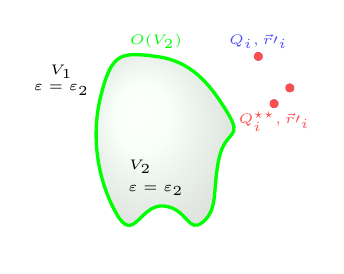
\begin{tikzpicture}[line width = 1.2pt, line join=round,>=stealth]
						\tiny;
		\filldraw [color=blue!70] (2.5,2.5) circle (1pt) node[above] {$Q_i, \vec{r}\prime _i$};
		\filldraw [color=blue!70] (2.9,2.1) circle (1pt);
		\filldraw [color=blue!70] (2.7,1.9) circle (1pt);
		\filldraw [color=red!70] (2.5,2.5) circle (1pt);
		\filldraw [color=red!70] (2.9,2.1) circle (1pt);
		\filldraw [color=red!70] (2.7,1.9) circle (1pt) node[below] {$Q_i^{\star\star}, \vec{r}\prime _i$};

		% Ladungsdichte
		\coordinate (a) at (2.1,1.8);
		\coordinate (b) at (2,1.2);
		\coordinate (c) at (1.8,0.4);
		\coordinate (d) at (1.3,0.6);
		\coordinate (e) at (0.7,0.5);
		\coordinate (f) at (0.5,2);
		\coordinate (g) at (1.2,2.5);
		\shade[ball color=white!10!green!20,opacity=0.20] plot [smooth cycle, tension = 1] coordinates {(a) (b) (c) (d) (e) (f) (g)};
		\draw [color=green] plot [smooth cycle, tension = 1] coordinates {(a) (b) (c) (d) (e) (f) (g)} node [sloped, above] {$O(V_2)$};
		\draw(1,1.1) node {$V_2$};
		\draw(1.2,0.8) node{$\varepsilon=\varepsilon_2$};
		\draw(0,2.2) node[align=center] {$V_1$\\$\varepsilon=\varepsilon_2$};
	\end{tikzpicture}}
\end{minipage}


		  	In \ref{Grenz} war der Normalenvektor $\vec{n}$ von Medium 1 nach Medium 2 orientiert. Damit kann man einen Vektor in eine Tangential- und eine Normalkomponente zerlegen:
		  	 $\vec{a} = a_n \vec{n} + a_t \frac{(\vec{n}\times \vec{a})\times\vec{n}}{\abs{\vec{n}\times \vec{a}}} = (\vec{a}\cdot\vec{n}) \vec{n} + (\vec{n}\times \vec{a})\times\vec{n}$.
		  	 \ref{tanE} zeigt, dass die Tangentialkomponente von $E$ \textbf{immer stetig} ist:
		  	\begin{equation}
		  		\boxed{\vec{n} \times \left( \vec{E}_2 - \vec{E}_1\right) = \vec{0}} \Rightarrow \vec{E}_2 - \vec{E}_1 = (E_2\cdot\vec{n} - E_1\cdot\vec{n}) \vec{n}
		  	\end{equation}
		  	 Für das Skalarpotential folgt dann mit $\vec{E} = -\grad \phi$
		  	\begin{equation}\label{tanEpot}
		  		\boxed{\vec{n} \times \left( \grad \phi_1 - \grad \phi_2\right) = \vec{0}} \Rightarrow \grad \phi_1 - \grad \phi_2 = (\vec{n}\cdot\grad \phi_1 - \vec{n}\cdot\grad \phi_2) \vec{n}
		  	\end{equation}
		  	 Die Normalkomponente der Dielektrischen Verschiebung \textbf{kann unstetig sein} ($\nearrow$\ref{normD}): $\vec{n}\cdot (\vec{D} _2 - \vec{D} _1 ) = \rho_F$.  Hierzu muss es freie Ladungsträger geben. Für \textbf{ideale Dielektrika} gilt aber:
		  	\begin{equation}\label{normE}
		  		\vec{n}\cdot (\vec{D} _2 - \vec{D} _1 ) = 0 \Rightarrow \boxed{\vec{n}\cdot (\varepsilon_2\vec{E}_2 - \varepsilon_1\vec{E}_1 ) =0 } \text{ bzw. } \boxed{\vec{n}\cdot (-\varepsilon_2\grad \phi_2 + \varepsilon_1\grad \phi_1 ) =0 }
		  	\end{equation}
		  	 Ohne \enquote{innere Quellen} (also ohne zusätzlichen Potentialsprung, z.B. Dipolschicht) ist das \textbf{Potential zweimal stetig differenzierbar},  insbesondere gilt: 
		  	 \begin{equation}\label{stetpot}
		  	 	\boxed{\phi_2-\phi_1 = 0}
		  	 \end{equation}
		  	  Die Greenschen Funktionen des Freiraums in $V_1$ und $V_2$ sind:
		  	\begin{equation}
		  		G_{\varepsilon_1}(\vec{r} , \vec{r}' ) = \frac{1}{4\pi\varepsilon_1} \frac{1}{\abs{\vec{r}  - \vec{r}' }} \text{ bzw. }         G_{\varepsilon_2}(\vec{r} , \vec{r}' ) = \frac{1}{4\pi\varepsilon_2} \frac{1}{\abs{\vec{r}  - \vec{r}' }} \implies G_{\varepsilon_1}= \frac{\varepsilon_2}{\varepsilon_1} G_{\varepsilon_2}
		  	\end{equation}
		  	 Die Berechnung des Potentials einer Ladung in $V_1$ (erstes Ersatzproblem) erfolgt gemäß \ref{problemGreen}, wobei \ref{umwaelz} genutzt werden kann und $T,\lambda$ zunächst noch unbekannt sind:
		  	\begin{equation}\begin{split}
		  			\phi_1(\vec{r} ) & = Q G_{\varepsilon_1}(\vec{r} , \vec{r}' ) -  \lambda(\vec{r}' )Q^\star G_{\varepsilon_1}(\vec{r} , T(\vec{r}' ))\\
		  			& = Q G_{\varepsilon_1}(\vec{r} , \vec{r}' ) - \lambda(\vec{r} ) Q^\star G_{\varepsilon_1}(T(\vec{r} ), \vec{r}' )
		  	\end{split}\end{equation}
		  	 Beim zweiten Ersatzproblem liegt die Spiegelladung auf der Ursprungsladung, also gilt:
		  	\begin{equation}\begin{split}
		  			\phi_2(\vec{r} ) & = Q G_{\varepsilon_2}(\vec{r} , \vec{r}' ) +  Q^{\star\star} G_{\varepsilon_2}(\vec{r} , \vec{r}' )\\
		  			& = \left( Q +  Q^{\star\star}\right) G_{\varepsilon_2}(\vec{r} , \vec{r}' )
		  	\end{split}\end{equation}
		  	 Analog der \enquote{isolierten Kugel} kann keine zusätzliche Ladung ins Volumen gelangen. Wegen der Ladungserhaltung müssen sich also die Spiegelladungen kompensieren, weshalb gilt (die Gesamtladung, die für das Potential sorgt, bleibt konstant): \begin{equation}\boxed{-\lambda(\vec{r}' )Q^\star+Q^{\star\star}= 0}\end{equation}  Ziel ist nun $Q^\star$, $\lambda$ und $\vec{r} ^\star=T(\vec{r}' )$ ($Q^{\star\star}=\lambda Q^\star$) so zu bestimmen, dass die Stetigkeitsbedingungen auf $O(V_2)$ erfüllt werden. Mit \ref{stetpot} gilt überall, aber insbesondere auch auf $\vec{r} \in O(V_2)$ (wo $\lambda,T$ spezielle Eigenschaften haben):
		  	\begin{equation}\begin{split}
		  			0 \stackrel{!}{=}  (\phi_1 - \phi_2 ) & =   Q G_{\varepsilon_1}(\vec{r} , \vec{r}' ) - \underbrace{\lambda(\vec{r} )}_{=1} Q^\star G_{\varepsilon_1}(\underbrace{T(\vec{r} )}_{=\vec{r} }, \vec{r}' )
		  			-\left( Q +  Q^{\star\star}\right) G_{\varepsilon_2}(\vec{r} , \vec{r}' )\\
		  			& = \left( (Q-Q^\star) -(Q+Q^{\star\star})\frac{\varepsilon_1}{\varepsilon_2}   \right) G_{\varepsilon_1}(\vec{r} , \vec{r}' )\\
		  			0 &= \frac{Q-Q^\star}{\varepsilon_1} -\frac{Q+Q^{\star\star}}{\varepsilon_2} \Rightarrow \boxed{\frac{Q-Q^\star}{\varepsilon_1} = \frac{Q+Q^{\star\star}}{\varepsilon_2}}
		  	\end{split}\end{equation}
		  	 Gür die Tangentialkomponente des Feldes gilt auf $\vec{r} \in O(V_2)$ entsprechend \ref{tanEpot}:
		  	\begin{equation}\begin{split}
		  			\vec{0} & \stackrel{!}{=} \vec{n}\times \grad \phi_1 - \vec{n}\times \grad \phi_2 \\
		  			& = \vec{n}\times \grad \left[ Q G_{\varepsilon_1}(\vec{r} , \vec{r}' ) - \lambda(\vec{r} ) Q^\star G_{\varepsilon_1}(T(\vec{r} ), \vec{r}' ) \right]
		  			- \vec{n}\times \grad \left[ \left( Q +  Q^{\star\star}\right) G_{\varepsilon_2}(\vec{r} , \vec{r}' ) \right]\\
		  			& = \vec{n}\times \grad \left[ Q G_{\varepsilon_1}(\vec{r} , \vec{r}' ) - \lambda(\vec{r} ) Q^\star G_{\varepsilon_1}(T(\vec{r} ), \vec{r}' ) \right]
		  			- \vec{n}\times \grad \left[ \left( Q +  Q^{\star\star}\right) \frac{\varepsilon_1}{\varepsilon_2} G_{\varepsilon_1}(\vec{r} , \vec{r}' ) \right]
		  	\end{split}\end{equation}
		  	 Auf $\lambda$ und $T$ wird der Gradient angewendet. Es kann hier deshalb nicht einfach $\lambda(\vec{r} )=1$ und $T(\vec{r} )=\vec{r} $ für $\vec{r} \in O(V_2)$ verwendet werden ($\nabla 1=0; \text{ aber nicht offensichtlich }\nabla \lambda = 0$). Weiter gilt:
		  	\begin{equation}\begin{split}
		  			\vec{0} &= Q \; \vec{n}\times \grad G_{\varepsilon_1}(\vec{r} , \vec{r}' ) - Q^\star\; \vec{n}\times\grad \left( \lambda(\vec{r} ) G_{\varepsilon_1}(T(\vec{r} ), \vec{r}' ) \right)\\
		  			&\quad - \left( Q +  Q^{\star\star}\right) \frac{\varepsilon_1}{\varepsilon_2}\; \vec{n}\times \grad  G_{\varepsilon_1}(\vec{r} , \vec{r}' ) \\
		  			&= \left( Q  - \left( Q +  Q^{\star\star}\right) \frac{\varepsilon_1}{\varepsilon_2} \right)\; \vec{n}\times \grad G_{\varepsilon_1}(\vec{r} , \vec{r}' ) - Q^\star\; \vec{n}\times\grad \left( \lambda(\vec{r} ) G_{\varepsilon_1}(T(\vec{r} ), \vec{r}' ) \right)\\
		  			&= \left( Q  - \left( Q +  Q^{\star\star}\right) \frac{\varepsilon_1}{\varepsilon_2} \right)\; \vec{n}\times \grad G_{\varepsilon_1}(\vec{r} , \vec{r}' )  \\
		  			&\quad - Q^\star G_{\varepsilon_1}(T(\vec{r} ), \vec{r}' )\; \vec{n}\times\grad \lambda(\vec{r} ) - Q^\star\lambda(\vec{r} ) \; \vec{n}\times\grad G_{\varepsilon_1}(T(\vec{r} ), \vec{r}' ) \\
		  			&= \left( Q  - \left( Q +  Q^{\star\star}\right) \frac{\varepsilon_1}{\varepsilon_2} \right)\; \vec{n}\times \grad G_{\varepsilon_1}(\vec{r} , \vec{r}' )  \\
		  			&\quad - Q^\star G_{\varepsilon_1}(\vec{r} , \vec{r}' )\; \vec{n}\times\grad \lambda(\vec{r} ) - Q^\star \; \vec{n}\times\grad G_{\varepsilon_1}(T(\vec{r} ), \vec{r}' )
		  	\end{split}\end{equation}
		  	 $T$ ist stetig differenzierbar und es gilt $T(T(\vec{r} ))=\vec{r} $, deshalb ist: $\grad _{\vec{r} } G_{\varepsilon_1}(T(\vec{r} ), \vec{r}' )  = \grad _{T(\vec{r} )} G_{\varepsilon_1}(T(\vec{r} ), \vec{r}' )$.
		  	 Damit lässt sich der Ausdruck weiter zusammenfassen:
		  	\begin{equation}\begin{split}
		  			\vec{0} &= \underbrace{\left( \left(Q - Q^\star\right) - \left( Q +  Q^{\star\star}\right) \frac{\varepsilon_1}{\varepsilon_2} \right)}_{=0}\; \vec{n}\times \grad G_{\varepsilon_1}(\vec{r} , \vec{r}' )   - Q^\star G_{\varepsilon_1}(\vec{r} , \vec{r}' )\; \vec{n}\times\grad \lambda(\vec{r} )
		  	\end{split}\end{equation}
		  	 Somit gilt für $\vec{r} \in O(V_2)$:
		  	\begin{equation}
		  		{\vec{n}\times\grad \lambda(\vec{r} ) = \vec{0}}
		  	\end{equation}
		  	 Führt man gleichen Operationen mit der Stetigkeitsbedingung für die Normalkomponente ($\nearrow$ \ref{normE}) durch, so gilt für $\vec{r} \in O(V_2)$ auch:
		  	\begin{equation}
		  		{\vec{n}\cdot\grad \lambda(\vec{r} ) = 0}
		  	\end{equation}
		  	 Die Tangential- und die Normalkompontente sind 0, folglich gilt für $\vec{r} \in O(V_2)$:
		  	\begin{equation}
		  		\boxed{\grad \lambda(\vec{r} ) = \vec{0}}
		  	\end{equation}
		  	Man hat in der obigen Herleitung keine allgemeine Beziehung für das $\lambda$ gefunden, nur Anforderungen, die es erfüllen muss. Aber $\lambda (\vec{r} ) = 1$ (was in den Geometrien Ebene und Zylinder schon vorher verwendet wurde) erfüllt die letzte Beziehung. Mit $\lambda (\vec{r} ) = 1$ folgt:
		  	\begin{equation}
		  		Q^\star = Q^{\star\star} \text{ und } \frac{Q-Q^\star}{\varepsilon_1} = \frac{Q+Q^{\star}}{\varepsilon_2} \Rightarrow \boxed{Q^\star = \frac{\varepsilon_2-\varepsilon_1}{\varepsilon_2+\varepsilon_1} Q}
		  	\end{equation} 
		  Für das Beispiel der dielektrischen Spiegelung an einer Ebene soll hier damit weitergearbeitet werden. Dabei wird die leitende Ebene (s.o.) durch eine dielektrische Grenzfläche ersetzt.
		  	\begin{center}
		  		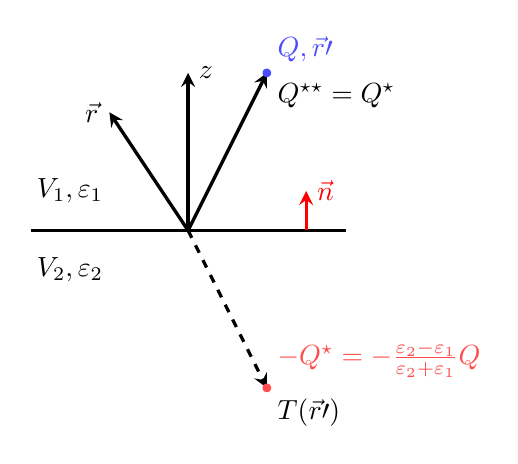
\begin{tikzpicture}[line width = 1.2pt, line join=round,>=stealth]
	\coordinate (O) at (0,0);
	\coordinate (a) at (-2,0);
	\coordinate (b) at (2,0);
	\draw (a) -- (b);
	\draw[color=red, -stealth] (1.5,0) -- (1.5,.5) node[right] {$\vec{n}$};
	\draw[ -stealth] (O) -- (0,2) node[right] {$z$};
	\draw[ -stealth] (O) -- (-1,1.5) node[left] {$\vec{r} $};
	\draw[ -stealth] (O) -- (1,2) node[below right] {$Q^{\star\star}=Q^\star$};
	\filldraw [color=blue!70] (1,2) circle (1pt) node[above right] {$Q, \vec{r}\prime $};
	\draw[ dashed, -stealth] (O) -- (1,-2) node[below right] {$T(\vec{r}\prime )$};
	\filldraw [color=red!70] (1,-2) circle (1pt) node[above right] {$-Q^\star=-\frac{\varepsilon_2-\varepsilon_1}{\varepsilon_2+\varepsilon_1} Q$};
	\draw(-1.5,0.5) node {$V_1,\varepsilon_1$};
	\draw(-1.5,-0.5) node {$V_2,\varepsilon_2$};

\end{tikzpicture}
		  	\end{center}
		  		 In $V_1$ gilt:
		  		\begin{equation}\label{spiegdielekt1}\begin{split}
		  				\phi_1(\vec{r} ) & = Q G_{\varepsilon_1}(\vec{r} , \vec{r}' ) -  Q^\star G_{\varepsilon_1}(\vec{r} , T(\vec{r}' ))\\
		  				& = Q\left( G_{\varepsilon_1}(\vec{r} , \vec{r}' ) -  \frac{\varepsilon_2-\varepsilon_1}{\varepsilon_2+\varepsilon_1} G_{\varepsilon_1}(\vec{r} , T(\vec{r}' ))\right)\\
		  				& = Q\frac{\varepsilon_0}{\varepsilon_1}\left( G(\vec{r} , \vec{r}' ) -  \frac{\varepsilon_2-\varepsilon_1}{\varepsilon_2+\varepsilon_1} G(\vec{r} , T(\vec{r}' ))\right)
		  		\end{split}\end{equation}
		  		 In $V_2$ gilt:
		  		\begin{equation}\label{spiegdielekt2}\begin{split}
		  				\phi_2(\vec{r} ) & = Q G_{\varepsilon_2}(\vec{r} , \vec{r}' ) +  Q^{\star\star} G_{\varepsilon_2}(\vec{r} , \vec{r}' )\\
		  				& = Q \left( 1 +  \frac{\varepsilon_2-\varepsilon_1}{\varepsilon_2+\varepsilon_1}\right) G_{\varepsilon_2}(\vec{r} , \vec{r}' ) \\
		  				& = Q\frac{\varepsilon_0}{\varepsilon_2} \left( 1 +  \frac{\varepsilon_2-\varepsilon_1}{\varepsilon_2+\varepsilon_1}\right) G(\vec{r} , \vec{r}' ) \\
		  				& = Q\frac{\varepsilon_0}{\varepsilon_1} \left( 1 -  \frac{\varepsilon_2-\varepsilon_1}{\varepsilon_2+\varepsilon_1}\right) G(\vec{r} , \vec{r}' )
		  		\end{split}\end{equation}
	  	Dividiert man noch durch $Q$ erhält man die problemangepassten Greenschen Funktionen für $V_1$ und $V_2$.
	  	\subsubsection{Weitere Szenarien für die Anwendung einer Spiegelung}
	  	In den vorigen Abschnitten wurde die Spiegelungsmethode für folgende Problemstellungen genutzt zur Spiegelung\dots
	  	\begin{itemize}
	  	\item[\dots] von \textbf{Ladungen} an \textbf{ideal leitenden} (geerdeten oder nicht geerdeten) Grenzflächen wie Kugel oder Ebene.
	  	\item[\dots] von \textbf{Ladungen} an \textbf{dielektrischen} Grenzflächen.
	  	\end{itemize}
	  	Analog kann man Spiegelungen auch für andere Problemstellungen nutzen. Beispiele sind die Spiegelung\dots
	  	\begin{itemize}
	  		\item[\dots] von \textbf{Dipolen} (und Multipolen) an \textbf{ideal leitenden} Grenzflächen. Dafür werden die Ladungen oder Ladungsdichten, die den Multipol bilden, als Ladungen gespiegelt. Modelliert man im Lösungsvolumen bspw. mit einem Punktdipol, wird auch auf der Spiegelseite wieder ein Punktdipol eingeführt.
	  		\item[\dots] von \textbf{Strömen} an \textbf{ideal leitenden} Grenzflächen. Dazu folgendes Beispiel: Oberhalb der Grenzfläche $z = 0$ ist Vakuum und unterhalb davon ist ein Material mit den linearen, homogenen, isotropen Parametern $\kappa\to\infty,\mu,\varepsilon$. Betrachtet wird ein Teilstück von einem Stromkreis, in dem der Gleichstrom $I$ von dem Punkt $P_+ (x = -a, y = 0, z = b > 0)$ zu dem Punkt $P_- (x = a, y = 0, z = b)$ fließt. Der Spiegelstrom fließt von dem Punkt $\hat{P_-}(x = a, y = 0, z = −b)$ zu dem Punkt $\hat{P_+}(x = -a, y =
	  		0, z = −b)$. Der Strom wird im Stromkreis durch eine EMK ($\nearrow$ \ref{Urspannung}) angetrieben, welche letztlich eine Ladungstrennung bewirkt. Der Strom fließt von $+\to -$, auch zwischen den gespiegelten Ladungen von der Ladungstrennung, welche das inverse Vorzeichen der Originalladungen haben.
	  		\item[\dots] von \textbf{Strömen} an \textbf{hochpermeablen} Grenzflächen. Dazu folgendes Beispiel: Oberhalb der Grenzfläche $z = 0$ ist Vakuum und unterhalb davon ist ein Material mit den linearen, homogenen, isotropen Parametern $\kappa,\mu\to\infty,\varepsilon$. Es gibt keine Oberflächenstromdichte. Betrachtet wird ein Teilstück von einem Stromkreis, in dem der Gleichstrom $I$ von dem Punkt $P_+ (x = -a, y = 0, z = b > 0)$ zu dem Punkt $P_- (x = a, y = 0, z = b)$ fließt. Der Spiegelstrom fließt von dem Punkt $\hat{P_+}(x = -a, y =
	  		0, z = −b)$ zu dem Punkt $\hat{P_-}(x = a, y = 0, z = −b)$. Das hat den Grund, dass \ref{tanH} erfüllt sein muss und $H$ im hochpermeablen Medium 0 ist (sonst hätte man wegen $w_m=\frac{1}{2}\mu H^2$ eine unendliche Energie). Also darf $H$ in der Spiegelebene keine Tangentialkomponente haben, was durch den so gewählten Spiegelstrom erreicht wird.
	  	\end{itemize}
 \subsection{Separationsansatz}\label{sep}
 Siehe auch \ref{pdglsep} für weitere Beispiele. Genutzt werden hier oft auch Orthogonalitätsbeziehugen, Reihenentwicklungen, ... nach \ref{orth}.\\
 Weiterhin soll die \textbf{Poisson-Gleichung}
	        \begin{equation}\begin{split}
			        \Delta \phi = -\frac{1}{\varepsilon_0} \rho(\vec{r} ) \text{ in } V
		        \end{split}\end{equation}
	        mit \textbf{Dirichlet-} und/oder \textbf{Neumann-Randbedingungen} auf der Oberfläche von $V$ gelöst werden:
	        \begin{equation}\begin{split}
			        \forall \vec{r} _{b} \in O(V) : \phi(\vec{r} _b) \veebar \left. \frac{\partial \phi}{\partial n}\right|_{\vec{r} =\vec{r} _b} \text{ vorgegeben}
		        \end{split}\end{equation}
	   In Fällen, in denen die Problemgeometrie gut zu den Symmetrien des Koordinatensystems passt, kann sich ein \textbf{Separationsansatz} bzw. \textbf{Produktansatz} lohnen (z.B. muss Lösungsgebiet in 2D durch Rechteck beschreibbar sein).
	   Ziel ist es hierbei, die partielle Differentialgleichung in ein System gewöhnlicher Differentialgleichungen zu überführen. Randbedingungen werden dann durch geeignete Anpassung der Konstanten berücksichtigt.
	   Der Ansatz für die Koordinaten $(x_1,x_2,x_3)$ lautet: \begin{equation}\boxed{\phi(\vec{r} )= f(x_1) \cdot g(x_2) \cdot h(x_3) }\end{equation}
  \subsubsection{Laplacegleichung in 2D mit Randbedingungen}
		   Folgendes 2D-Problem soll zunächst betrachtet werden:
		        \begin{itemize}
			        \item \textbf{Lösungsvolumen}: $ V = [0,x_0] \times [0,y_0]$ (Rechteck in der $x$-$y$-Ebene)
			        \item \textbf{Randwerte} (Dirichlet): $\phi(x,y) = 0$ für $x=0$, $x=x_0$ und $y=0$ sowie $\phi(x,y_0) = \phi_0(x)$
			        \item keine \textbf{Ladungen} in $V$, also $\boxed{\Delta \phi = 0 \text{ in } V}$
		        \end{itemize}
		   Mit dem Laplaceoperator $\Delta = \frac{\partial^2}{\partial x^2} + \frac{\partial^2}{\partial y^2}$ und dem \textbf{Ansatz} $\phi (x,y) = f(x)g(y)$
		        folgt:
		        \begin{equation}\begin{split}
				        \Delta \phi(x,y)   = \Delta \left[f(x)g(y)\right] = g(y)\frac{\dd^2 f(x)}{\dd x^2} + f(x)\frac{\dd^2 g(y)}{\dd y^2} &= 0\\
				        \frac{1}{f(x)}\frac{\dd^2 f(x)}{\dd x^2} + \frac{1}{g(y)}\frac{\dd^2 g(y)}{\dd y^2} &= 0\quad (\text{für } \phi\neq 0)
			        \end{split}\end{equation}
		   Offensichtlich müssen die beiden Summanden sich gegenseitig aufheben:
		        \begin{equation}\begin{split}
				        \boxed{- \frac{1}{f(x)}\frac{\dd^2 f(x)}{\dd x^2}  = k^2 =  \frac{1}{g(y)}\frac{\dd^2 g(y)}{\dd y^2}} \in \mathbb{R}
			        \end{split}\end{equation}
		   Ein positiver Wert (oder Null $\to$ Triviallösung kann Randbedingungen nicht erfüllen) für $\frac{1}{f(x)}\frac{\dd^2 f(x)}{\dd x^2}$ führt auf den gegebenen Randbedingungen zu keiner Lösung. Würde man das negative Vorzeichen bei $g$ setzen, dann würde man zu keiner Lösung kommen, die zu den Randbedingungen passt. Da bei $x=0$ bzw. $x=x_0$ der Wert 0 ist, passt die sin/cos-Lösung besser zur $x$-Richtung (wie eingespannte Saite $\to$ sin/cos haben mehrere Nullstellen). Die allgemeine Lösung ist:
		        \begin{align}
			        f''(x) & = - k^2 f(x) & f(x) & = \alpha \sin(kx) + \beta \cos(kx)  \\
			        g''(y) & = k^2 g(y)   & g(y) & = \gamma\sinh(ky) + \delta\cosh(ky)
		        \end{align}
		   Randbedingungen \enquote{links} ($x=0$), \enquote{unten} ($y=0$) und \enquote{rechts} ($x=x_0$):
		        \begin{align}
			        \phi(x=0,y)    & = 0 & \beta            & =0                                                     \\
			        \phi(x,y=0)    & =0  & \delta           & = 0                                                    \\
			        \phi(x=x_0, y) & = 0 & \alpha\sin(kx_0) & = 0 \Rightarrow k=k_n=\frac{n\pi}{x_0};\,n\in\mathbb{N}
		        \end{align}
		   Die vollständige Lösung - die aber noch nicht die Randbedingung \enquote{oben} erfüllt, ist daher (Superposition aller möglichen Lösungen):
		        \begin{equation}\begin{split}
				        \phi(x,y) = \sum_{n\in\mathbb{N}} c_n \sin\left( \frac{n\pi}{x_0} x \right) \sinh\left( \frac{n\pi}{x_0} y \right)
			        \end{split}\end{equation}
		   Für die Randbedingung \enquote{oben} muss gelten:
		        \begin{equation}\begin{split}
				        \phi(x,y=y_0) = \phi_0(x) &= \sum_{n\in\mathbb{N}} c_n \sin\left( \frac{n\pi}{x_0} x \right) \sinh\left( \frac{n\pi}{x_0} y_0 \right)
			        \end{split}\end{equation}
		   Zum Auflösen nach $c_n$ muss die Summe auf einen Term reduziert werden.
		   Dazu kann die \textbf{Orthogonalität} ($\nearrow$\ref{orth}) genutzt werden. Multiplikation mit \textcolor{red}{$\sin\left( \frac{m\pi}{x_0} x \right)$} und \textcolor{green}{Integration über $[0,x_0]$} liefert\footnote{\label{anmSEP}\textbf{Anmerkung:} In diesem Fall ist $[0,x_0]$ das einzige Intervall \textbf{im Lösungsgebiet}, in dem die $\sin$ untereinander Orthogonalität haben ($\langle\sin\left( \frac{m\pi}{x_0} x \right),\sin\left( \frac{n\pi}{x_0} x \right)\rangle_{[0,x_0]}=\frac{x_0}{2}\delta_{mn}$), also das einzig sinnvolle Integrationsintervall. Aber: $\sin\left( \frac{m\pi}{x_0} x \right)$ hat als Grundperiode $2x_0$. Entsprechend ist bspw. $\langle\sin\left( \frac{m\pi}{x_0} x \right),\cos\left( \frac{n\pi}{x_0} x \right)\rangle_{[0,x_0]}=0$ \textbf{nicht} für alle $m,n$ gegeben. Grundsätzlich kann man natürlich Skalarprodukte von beliebigen Funktionen auf beliebigen Intervallen bilden, jedoch muss man aufpassen, dass man nicht fälschlicherweise Orthogonalität annimmt.}:
		        \begin{equation}\begin{split}
				        \phi_0(x) \textcolor{red}{\sin\left( \frac{m\pi}{x_0} x \right)} &= \sum_{n\in\mathbb{N}} c_n \sin\left( \frac{n\pi}{x_0} x \right) \textcolor{red}{\sin\left( \frac{m\pi}{x_0} x \right)} \sinh\left( \frac{n\pi}{x_0} y_0 \right) \\
				        \textcolor{green}{\int\limits_0^{x_0}} \phi_0(x) \textcolor{red}{\sin\left( \frac{m\pi}{x_0} x \right)} \textcolor{green}{\dd x} &=
				        \sum_{n\in\mathbb{N}} c_n \underbrace{\textcolor{green}{\int\limits_0^{x_0}} \sin\left( \frac{n\pi}{x_0} x \right) \textcolor{red}{\sin\left( \frac{m\pi}{x_0} x \right)} \textcolor{green}{\dd x}}_{\frac{x_0}{2}\delta_{mn}} \sinh\left( \frac{n\pi}{x_0} y_0 \right) \\
				        c_n &= \frac{2}{x_0 \sinh\left( \frac{n\pi}{x_0} y_0 \right)}  \int\limits_0^{x_0} \phi_0(x) \sin\left( \frac{n\pi}{x_0} x \right) \dd x
			        \end{split}\end{equation}
		        Mit $c_n$ ist die vollständige Lösung in Form einer Reihe angebbar, wobei $c_n$ so bestimmt wurde, dass die Randbedingungen eingehalten werden.
  \subsubsection{Poissongleichung mit Randbedingungen}
  Nun wird ein 3D-Problem betrachtet:
  \begin{itemize}
		   \item \textbf{Lösungsvolumen}: $V = [-\infty,\infty] \times [0,d]\times [-\infty,\infty]$
		  \item  \textbf{Randwerte}: $\phi(x,y=0,z)=\phi(x,y=d,z) = 0$
		   \item \textbf{Quelle}: Es ist eine konstante Ladungsdichte parallel zur $z$-Achse gegeben mit $\rho_\text{V} (\vec{r} )
			        = \rho_L \delta(x-x_0)\delta(y-y_0)$. Diese liegt bei $x_0 \text{ beliebig};\; y_0
			        \in (0,d)$.
\end{itemize}
		   Es gibt eine \textbf{Translationsinvarianz} in $z$-Richtung. Die Lösung ist also unabhängig von $z$, das Problem reduziert sich auf ein \textbf{2D}-Problem:
		        \begin{equation}\begin{split}
				        \phi(x,y,z) = \phi(x,y); \; V\to A= [-\infty,\infty] \times [0,d]; \; \rho_\text{V} \to \rho_F(x,y) = q \delta(x-x_0)\delta(y-y_0)
			        \end{split}\end{equation}
		   Eine Möglichkeit dieses Problem zu behandeln ist die Formale Lösung, also die problemangepasste Greensche-Funktion z.B durch (unendliche) Spiegelung zu ermitteln. Eine andere Möglichkeit ist das Aufteilen des Lösungsgebietes in den Bereich $A_-$ \enquote{links} von $x=x_0$ und den Bereich $A_+$ \enquote{rechts} von $x=x_0$, also:
		        \begin{equation}\label{auft}\begin{split}
				        A_- &= \{\vec{r}  = (x,y)\; |\; x<x_0 \land 0\le y\le d \} \\
				        A_+ &= \{\vec{r}  = (x,y)\; |\; x>x_0 \land 0\le y\le d \}
			        \end{split}\end{equation}
		   Durch die Aufteilung in $A_-$ und $A_+$ muss dort \enquote{nur} noch die Laplace-Gleichung gelöst werden
		        \begin{equation}\begin{split}
				        \Delta \phi_-  (x,y) = 0 \text{ für } (x,y) \in A_- ;\quad \Delta \phi_+ (x,y) = 0 \text{ für } (x,y) \in A_+
			        \end{split}\end{equation}
		   mit den Randbedingungen
		        \begin{itemize}
			        \item $\phi_\pm (x, y=0) = \phi_\pm(x,y=d) = 0 $ (Dirichlet)
			        \item $\left. -\varepsilon_0\left( \frac{\partial \phi_+}{\partial x} -\frac{\partial \phi_-}{\partial x} \right)\right|_{x=x_0} = q\delta(y-y_0)=\sigma(y)$ (Neumann, wegen \ref{normD})
			        \item $\phi_-(x\to-\infty) = 0 = \phi_+(x\to+\infty) $ (Randbedingungen im Unendlichen)
		        \end{itemize}
		   Nun wird der Produktansatz in der $x$-$y$-Ebene angesetzt, also $\phi_\pm(x,y) = f(x)\cdot g(y)$. Hier ist nun bei $y=0$ und bei $y=d$ $\phi=0$, also ist es sinnvoll, dass in $y$-Richtung die sin/cos-Lösung entsteht (negatives Vorzeichen vor $g$). Umformen der Laplace-Gleichung liefert: 
		        \begin{equation}\begin{split}
		        		\frac{1}{f(x)}\frac{\dd^2 f(x)}{\dd x^2}  &= k^2 =  -\frac{1}{g(y)}\frac{\dd^2 g(y)}{\dd y^2}\\
				        \Rightarrow f(x) &= \alpha e^{kx} + \beta e^{-kx} \\
				       \Rightarrow g(y) &= \gamma\sin(ky) + \delta\cos(ky); \quad k>0 
			        \end{split}\end{equation}
		        Die Einschränkung $k>0$ ist ohne Beschränkung der Allgemeinheit möglich, denn sofern eine Lösung gefunden wird, die die Randbedingungen erfüllt, ist dies eindeutig. Es gilt:
		        \begin{itemize}
		        	\item $\phi_\pm(x,y=0) = 0 \Rightarrow {\delta=0}$
		        	\item $\phi_\pm(x,y=d) = 0 \Rightarrow {k=k_n = \frac{n\pi}{d}} \text{ für } n\in\mathbb{N}$
		        \end{itemize}
		   Die Lösung soweit ist also: 
		   \begin{equation}\phi_\pm(x,y) = \sum_{n=1}^\infty \hat{C}_n^\pm \left[\alpha e^{\frac{n\pi}{d} x} + \beta e^{-\frac{n\pi}{d} x}\right]\gamma \sin\left(\frac{n\pi}{d} y\right) 
		   \end{equation}
		   Anwendung der Randbedingungen im Unendlichen:
		   \begin{itemize}
		   	\item $\phi_-(x\to -\infty, y) = 0 \Rightarrow \beta=0$ in $\phi_-$ 
		   	\item $\phi_+(x\to \infty, y) = 0 \Rightarrow \alpha=0$ in $\phi_+$ 
		   \end{itemize}
		   $\alpha$ bzw. $\beta$ sind Konstanten, sie können mit den Konstanten $\hat{C}_n^\pm$ zusammengefasst werden. Die Lösung bis hierhin ergibt sich zu:
		        \begin{equation}\begin{split}
				        \phi_\pm(x,y) = \sum_{n=1}^\infty C_n^\pm e^{\mp\frac{n\pi}{d} x} \sin\left(\frac{n\pi}{d} y\right)
			        \end{split}\end{equation}
		   Die Lösung muss bei $x=x_0$ stetig sein:
		        \begin{equation}\begin{split}
				        \sum_{n=1}^\infty C_n^+ e^{-\frac{n\pi}{d} x_0} \sin\left(\frac{n\pi}{d} y\right) = \sum_{n=1}^\infty C_n^- e^{+\frac{n\pi}{d} x_0} \sin\left(\frac{n\pi}{d} y\right)
			        \end{split}\end{equation}
		   Dies erfordert:
		        \begin{equation}\begin{split}
				        C_n^+ e^{-\frac{n\pi}{d} x_0} = C_n^- e^{+\frac{n\pi}{d} x_0} = A_n; \; \forall n\in\mathbb{N}
			        \end{split}\end{equation}
		   Ersetzen von $C_n^\pm$ durch $A_n$ führt zu:
		        \begin{equation}\begin{split}
				        \phi_\pm(x,y) = \sum_{n=1}^\infty A_n e^{-\frac{n\pi}{d} |x-x_0|} \sin\left(\frac{n\pi}{d} y\right)
			        \end{split}\end{equation}
		   Mit $\left. -\varepsilon_0\left( \frac{\partial \phi_+}{\partial x} -\frac{\partial \phi_-}{\partial x} \right)\right|_{x=x_0} = q\delta(y-y_0)=\sigma(y)$ und der Orthonormalitätsbeziehung folgt:
		        \begin{equation}\begin{split}
				        A_n &= \frac{q}{\varepsilon_0 \pi} \frac{\sin\left(\frac{n\pi}{d}y_0\right)}{n} \\
				        \phi(x,y) &= \frac{q}{\varepsilon_0 \pi}  \sum_{n=1}^\infty \frac{1}{n} \sin\left(\frac{n\pi}{d}y_0\right)  \sin\left(\frac{n\pi}{d}y\right)  e^{-\frac{n\pi}{d} |x-x_0|} \\
				         \vec{E} &= -\grad \phi
			        \end{split}\end{equation}
\subsection{Orthogonale Funktionensysteme}\label{elorth}
Für geeignete Geometrien kann das Potential allgemein in eine Reihe von Basisfunktionen (welche ein vollständiges Funktionensystem bilden) des Raumes der quadratintegrierbaren Funktionen entwickelt werden, das Potential kann also zunächst jede beliebige $L^2$-Funktion sein ($\nearrow$\ref{orth}). Diese Reihe muss an die gegebenen Randbedingungen sukzessive angepasst werden. Dabei kann es erforderlich sein, den Raum sinnvoll in Teilräume zu spalten.
  \subsubsection{Geladene Kugelfläche}
		   Nun soll das Potential einer geladenen Kugelfläche mit Radius $R$ und \textbf{rotationssymmetrischer} Ladungsverteilung betrachtet werden:
		        \begin{equation}\begin{split}
				        \rho_\text{V} (\vec{r} ) =\rho_\text{V} (r,\vartheta,\varphi) = \rho_\text{F} (\textcolor{red}{\vartheta}) \delta(r-R) = \sigma(\vartheta) \delta(r-R)
			        \end{split}\end{equation}
		   Auch hier wird das Problem wieder in \enquote{innen} und \enquote{außen} unterteilt, wobei auf beiden Seiten nur die Laplace Gleichung betrachtet werden muss. Aus der Ladungsverteilung auf der Oberfläche folgt mit \ref{normD} eine Neumann Randbedingung bei $R$. Die Kugelflächenfunktionen bilden wie in \ref{orth} erwähnt ein vollständiges Funktionensystem auf der Einheitskugel, jede beliebige quadratintegrable Funktion kann in die Folgende Darstellung entwickelt werden ($\nearrow$\ref{entwicklungKugelf}):		        \begin{equation}\begin{split}
				        \phi(r, \vartheta,\varphi) &= \sum_{l=0}^{\infty}\sum_{m=-l}^l  (A_{lm} r^l+ B_{lm} r^{-(l+1)}) Y_{lm}(\vartheta,\varphi)\quad \text{ mit } \\Y_{lm}(\vartheta,\varphi)&= \sqrt{\frac{2l+1}{4\pi}\frac{(l-m)!}{(l+m)!}} P_{lm}(\cos\vartheta) e^{jm\varphi}
			        \end{split}\end{equation}
		  Das Problem ist \textbf{rotationssymmetrisch} bezüglich $\varphi$, also kann die Lösung nicht von $\varphi$ abhängen $\implies m=0$. Außerdem sind $A$ und $B$ zunächst (nur von $l$) abhängige Konstanten, alles was an Faktoren nur von $l$ abhängt kann also durch zusammenziehen von Konstanten beliebig verändert werden:
		        \begin{equation}\begin{split}
				        \phi(r, \vartheta,\varphi) = \phi(r, \vartheta) &= \sum_{l=0}^{\infty} (A'_{l} r^l+ B'_{l} r^{-(l+1)}) Y_{l0}(\vartheta,\varphi)\\
				        &= \sum_{l=0}^{\infty} (A'_{l} r^l+ B'_{l} r^{-(l+1)}) \sqrt{\frac{2l+1}{4\pi}} \underbrace{P_{l0}(\cos\vartheta)}_{P_l (\cos\vartheta)}\\
				        & = \sum_{l=0}^{\infty} (A_{l} r^l+ B_{l} r^{-(l+1)}) \frac{2l+1}{2} P_l (\cos\vartheta)
			        \end{split}\end{equation}
		   Dabei sind $P_{l0}(x) = P_l(x)$ die \textbf{Legendre-Polynome}, welche ein vollständiges System auf $[-1,1]$ bilden:
		        \begin{equation}\begin{split}
				        P_{l0}(x) = P_l(x) = \frac{1}{2^l l!} \frac{\dd^l}{\dd x^l} (x^2-1)^l 
			        \end{split}\end{equation}
		   Es gilt folgende Orthogonalitätsrelation:
		        \begin{equation}\begin{split}
				        \int\limits_{-1}^1 P_l(x)P_m(x) \dd x = \frac{2}{2l+1} \delta_{lm}
			        \end{split}\end{equation}
		   Da die Legendre-Polynome ein vollständiges System auf $[-1,1]$ (bezüglich $\cos\vartheta$ also $[0,\pi]$) sind, kann auch die Oberflächenladungsdichte nach diesen entwickelt werden:
		        \begin{equation}\begin{split}
				        \sigma(\vartheta) = \sum_{l=0}^{\infty}  \frac{2l+1}{2} \sigma_l P_l (\cos\vartheta)
			        \end{split}\end{equation}
		   Multiplikation mit $P_m$, Integration und Nutzung der Orthogonalitätsrelation liefert:
		        \begin{equation}\begin{split}
				        \sigma_l = \int\limits_{-1}^{1} \sigma(\vartheta) P_l(\cos\vartheta) \dd \cos\vartheta
			        \end{split}\end{equation}
		   Offensichtlich sollte das Potential (im unendlichen 0, bei 0 nicht unendlich $\to$ schwierig mit $r^i$) aufgeteilt werden in
		        \begin{equation}\begin{split}
				        \phi(\vec{r} ) = \phi(r,\vartheta) = \begin{cases}
					        \phi_- (r,\vartheta) = \sum_{l=0}^{\infty} (A_{l}^- r^l+ B_{l}^- r^{-(l+1)}) \frac{2l+1}{2} P_l (\cos\vartheta) & \text{ für } r < R \\
					        \phi_+ (r,\vartheta)=\sum_{l=0}^{\infty} (A_{l}^+ r^l+ B_{l}^+ r^{-(l+1)}) \frac{2l+1}{2} P_l (\cos\vartheta)   & \text{ für } r > R
				        \end{cases}
			        \end{split}\end{equation}
		   Nun können die Randbedingungen genutzt werden:
		   \begin{itemize}
		   	\item Es gibt keine Ladung im Ursprung $\to$ keine Singularität von $\phi_-(r\to 0) \Rightarrow \boxed{B_l^- =0}$
		   	\item Das Potential verschwindet im Unendlichen $\phi_+(r\to \infty) = 0  \Rightarrow \boxed{A_l^+ =0}$
		   	\item Stetigkeit bei $r=R$: $\left. A_{l}^- r^l\right|_{r=R} = \left. B_{l}^+ r^{-(l+1)}\right|_{r=R} \Rightarrow \boxed{B_{l}^+ = A_{l}^- R^{2l+1} } $
		   	\item Neumann-Randbedingung:
		        \begin{equation}\begin{split}
				        \sigma(\vartheta) &= -\varepsilon_0 \left.\left( \frac{\partial \phi_+}{\partial r} - \frac{\partial \phi_-}{\partial r}\right)\right|_{r=R} \\
				        & = \left. -\varepsilon_0 \sum_{l=0}^{\infty} \left( -(l+1) A_{l}^- R^{2l+1} r^{-(l+2)}- l A_{l}^- r^{l-1}\right) \frac{2l+1}{2} P_l (\cos\vartheta) \right|_{r=R} \\
				        &= \varepsilon_0 \sum_{l=0}^{\infty} \frac{(2l+1)^2}{2} A_{l}^- R^{l-1} P_l (\cos\vartheta)
			        \end{split}\end{equation}
		   \item[]$\to$Es gilt die Entwicklung $\sigma(\vartheta) = \sum_{l=0}^{\infty}  \frac{2l+1}{2} \sigma_l P_l (\cos\vartheta)$, also liefert ein Termvergleich:
		        \begin{equation}\begin{split}
				        \varepsilon_0 (2l+1) A_{l}^- R^{l-1} = \sigma_l \Rightarrow \boxed{ A_{l}^- = \frac{1}{(2l+1)\varepsilon_0}\sigma_l  R^{-(l-1)}}
			        \end{split}\end{equation}
		        		   \end{itemize}
		   Damit ist die Gesamtlösung gefunden:
		        \begin{equation}\label{GesamtLsg}\begin{split}
				        \phi(\vec{r} ) = \phi(r,\vartheta) =
				        \begin{cases}
					        \phi_-(r,\vartheta) & = \frac{R}{\varepsilon_0} \sum_{l=0}^{\infty} \frac{\sigma_l}{2} \left(\frac{r}{R}\right)^l P_l(\cos\vartheta) \text{ für } r<R     \\
					        \phi_+(r,\vartheta) & = \frac{R}{\varepsilon_0} \sum_{l=0}^{\infty} \frac{\sigma_l}{2} \left(\frac{R}{r}\right)^{l+1} P_l(\cos\vartheta) \text{ für } r>R 
				        \end{cases}
			        \end{split}\end{equation}
		   \ref{entwicklungKugelf} ist die allgemeine Lösung der homogenen Laplace-Gleichung in Kugelkoordinaten. Das Lösungsgebiet wird also im Endeffekt wie in \ref{auft} in zwei Lösungsgebiete ohne Inhomogenität geteilt, in denen die Laplace-Gleichung gelöst wird und anschließend wird diese allgemeine Lösung der Laplace-Gleichung an die Randbedingungen angepasst. Diese Lösungsmethodik ist also eng mit \ref{sep} verwandt.\\\\
	  \textbf{Einfachster Fall- homogen geladene Kugel:}\\
			   Bei einer homogenen Kugel gilt: $\sigma(\vartheta) = \sigma = \frac{Q}{4\pi R^2}$. Das muss entwickelt werden:
			        \begin{equation}\begin{split}
					        \frac{Q}{4\pi R^2} & = \sum_{l=0}^\infty \frac{2l+1}{2}\sigma_l P_l(\cos(\vartheta)) \stackrel{l=0}{=} \frac{\sigma_0}{2}\\
					        \sigma_0 &= \frac{2Q}{4\pi R^2}
				        \end{split}\end{equation}
			   Das kann in \ref{GesamtLsg} eingesetzt werden und man erhält (E-Feld nach Gradientenbildung):
			        \begin{align}
				        \phi_-(r)     & = \frac{Q}{4\pi\varepsilon_0 R} & \phi_+(r)     & = \frac{Q}{4\pi\varepsilon_0 r}                    \\
				        \vec{E}_- (r) & = \vec{0}                       & \vec{E}_+ (r) & = \frac{Q}{4\pi\varepsilon_0} \frac{\vec{r} }{r^3}
			        \end{align}
 \section{Materie}\label{materie}
		   Die Maxwellgleichungen für das Vakuum gelten zunächst auch \textbf{unverändert} in Materie, wie in \ref{mat} bereits festgestelt wurde. Das liegt daran, dass Materie \enquote{Nichts + Elementarteilchen} ist. Elementarteilchen sind Protonen, Neutronen und Elektronen. Ebenen darunter, also Quarks..., werden hier nicht betrachtet. Materie ist sehr \enquote{dünn}, was an folgendem Beispiel verdeutlicht werden soll:\\
			         \textit{Das dichteste Element ist {Osmium} (Os) mit einer Ordnungszahl von $76$, einer Dichte von $22.6\; \frac{\mathrm{g}}{\mathrm{cm}^3}$ und einer Atommasse von $190.23 \mathrm{u}$ . Daraus kann man berechnen, dass $1$ Mol Osmium $8.4\; \mathrm{cm}^3$ entspricht.
			         Mit den Radien (Kugelannahme ist nicht unproblematisch!) von Elektron ($\approx 10^{-19}\mathrm{m}$), Proton und Neutron (jeweils $\approx 10^{-15}$\;m) rechnet man aus, dass $1$ Mol Osmium etwa $0.5\cdot 10^{-12}\;\mathrm{cm}^3$ \enquote{reiner} Materie enthält.
			         Oder anders ausgedrückt: In $16.8\;(\mathrm{hm})^3$ ist $1\;\mathrm{cm}^3$ \enquote{reine} Materie.}\\
		   Man könnte in Materie mit den Maxwell-Gleichungen des Vakuums rechnen, müsste dann aber über alle Ladungen superponieren und dabei die Orte und Ortsveränderung aller Ladungen immer berücksichtigen. Die Informationen hierzu sind erstens gar nicht einfach verfügbar und zweitens sind die dann berechenbaren Details gar nicht beobachtbar. Deshalb geht man von den \textbf{mikroskopischen} (Teilchen einzeln betrachtet) zu \textbf{makroskopischen Betrachtungen} über. 
  \subsection{Makroskopische Größen}
  Größere Ladungsansammlungen (Atome, Ionen, Moleküle, ...) können als Ladungsanhäufungen (\enquote{Teilchen}) betrachtet werden, zwischen denen fast nichts ist.
  \subsubsection{Ladungsdichte, Dipolmoment und Skalarpotential von einem \enquote{Teilchen}}
   Befinden sich im $k$-ten \enquote{Teilchen} die Ladungen  $q_i^k$ ($i$-te Ladung im $k$-ten Teilchen, gebunden oder frei) an den Orten $r_i = r_i(t)$, so ist die \textbf{Ladungsdichte im Bereich des $k$-ten Teilchens} in guter Näherung  (der Einfluss von benachbarten \enquote{Teilchen} verschwindet näherungsweise wegen der großen Entfernung):
		        \begin{equation}\begin{split}
				        \rho^k(\vec{r} , t) = \sum_i q_i^k \delta^3(\vec{r}  - \vec{r} _i(t) ) \quad \stackrel{\text{zeitl. Mittlung}}{\longrightarrow} \quad \boxed{\rho^k(\vec{r} ) = \sum_i q_i^k \delta^3(\vec{r}  - \vec{r} _i )}
			        \end{split}\end{equation}
		   Ist $\vec{R}^k=\vec{R}^k(t)$ der \textbf{Ladungsschwerpunkt} des $k$-ten Teilchens, so ergibt sich das \textbf{Dipolmoment} zu:
		        \begin{equation}\begin{split}
				        \vec{p}^k(t) = \int\limits_{V^k} \rho^k(\vec{r} , t) (\vec{r}  - \vec{R}^k(t) ) \dd^3r \quad \stackrel{\text{zeitl. Mittlung}}{\longrightarrow} \quad \boxed{\vec{p}^k = \int\limits_{V^k} \rho^k(\vec{r} ) (\vec{r}  - \vec{R}^k ) \dd^3r}
			        \end{split}\end{equation}
		  Die Abstände innerhalb der \enquote{Teilchen} sind in aller Regel sehr klein im Vergleich zum Abstand zwischen Ladungsschwerpunkt und Beobachtungspunkt, also $|\vec{r} ^k -  \vec{R}^k| \ll  |\vec{r}  - \vec{R}^k | \text{ für } \vec{r} ^k \in V^k $. Um das \textbf{Skalarpotential des $k$-ten \enquote{Teilchens}} zu errechnen ist es näherungsweise wegen der großen Entfernung sinnvoll, die Multipolentwicklung ($\nearrow$ \ref{multi}) nach dem Dipolterm abzubrechen ($q^k\hat{=}$ Gesamtladung des $k$-ten Teilchens):
		        \begin{equation}\begin{split}
				        \phi^k(\vec{r} ) \approx \frac{1}{4\pi\varepsilon_0} \left[ \frac{q^k}{|\vec{r}  - \vec{R}^k |} + \frac{\vec{p}^k \cdot (\vec{r}  - \vec{R}^k )}{|\vec{r}  - \vec{R}^k |^3} \right]
			        \end{split}\end{equation}
  \subsubsection{Ladungsdichte, Dipolmoment und Skalarpotential von $N$ \enquote{Teilchen}}
		   Für $N$ \enquote{Teilchen} ergeben sich dann \textbf{effektive} Ladungsdichte, Dipoldichte und Potential in  der Form
		        \begin{equation}\begin{split}
				        \rho_{\text{eff}}(\vec{r} ) & = \sum_{k=1}^N q^k\delta (\vec{r}  - \vec{R}^k ) \quad\text{mit Gesamtladung } q^k\\
				        \vec{p}_{\text{eff}}(\vec{r} ) &= \sum_{k=1}^N \vec{p}^k\delta (\vec{r}  - \vec{R}^k ) \quad\text{mit Gesamtdipolmoment } \vec{p}^k\\
				        \phi _{\text{eff}}(\vec{r} ) &= \frac{1}{4\pi\varepsilon_0} \int\limits_V \left[ \frac{\rho_{\text{eff}}(\vec{r}' )}{|\vec{r}  - \vec{r}'  |} + \frac{\vec{p}_{\text{eff}}(\vec{r}' )  \cdot (\vec{r}  - \vec{r}'  )}{|\vec{r}  - \vec{r}'  |^3} \right] \dd^3 r'
			        \end{split}\end{equation}
\subsubsection{Übergang von effektiven Größen zu makroskopischen Größen}
		   Aus den effektiven Größen ergeben sich die {makroskopischen} Größen durch Mittlung:
		   \begin{itemize}
		   	\item Die \textbf{makroskopische Ladungsdichte} ist gegeben mit $\rho_\text{V}(\vec{r} ) = \overline{\rho_{\text{eff}}(\vec{r} )} $\footnote{$\overline{u\left( \vec{r},t \right)}=\frac{1}{V}\int\limits_{V}{u\left( \vec{r}+\vec{r}\,',t \right)\mathrm{d}}^3r'\to u\left( \vec{r},t \right)$ ist die mikroskopische Größe, $V$ ist ein Raumvolumen um $\vec{r}$, welches mikroskopisch groß, makroskopisch aber klein ist. $\rho_{V}$ enthält also noch die Ladungen, die sich bei der Mittlung nicht kompensiert haben. Dies sind die \enquote{freien} Ladungen. Die \enquote{Polarisationsladungen}, welche bei dieser Mittlung verschwinden, sorgen für die makroskopische Polarisation.\\
		   	Also steht in in $\div \vec{D}(\vec{r} ) = \rho_\text{V}(\vec{r} )$ nur die \enquote{Nettoladung} (also die Ladung die sich nicht kompensiert hat). Möchte man das elektrische Feld berechen, muss man beachten, dass dieses neben einer Komponente herrührend von der \enquote{Nettoladung} auch noch eine Komponente herrührend von der Polarisation des Mediums hat, also: $\vec{E}=\frac{\vec{D}-\vec{P}}{\varepsilon_{0}}=\vec{E}_\text{frei}+\vec{E}_\text{Polarisation}$.}, es werden alle Ladungen berücksichtigt, aber die meisten kompensieren sich in ihrer Wirkung.
		   	\item Die \textbf{makroskopische Polarisation} ergibt sich durch $\vec{P}(\vec{r} ) = \overline{\vec{p}_{\text{eff}}(\vec{r} )} $. Es werden \textit{Modelle} (zu dem Stoff passend: gewöhnliches Dielektrikum verhält sich anders als Kristall mit Vorzugsachse) benötigt, um die makroskopische Polarisation als Antwort auf interne und externe Felder vorherzusagen.
		   	\item Das \textbf{makroskopische Skalarpotential} ist dann
		   \end{itemize}
		        \begin{equation}\begin{split}
				        \phi (\vec{r} ) = \overline{\phi _{\text{eff}}(\vec{r} )} &= \frac{1}{4\pi\varepsilon_0} \int\limits_V \left[ \frac{\rho_\text{V}(\vec{r}' )}{|\vec{r}  - \vec{r}'  |} + \frac{\vec{P}(\vec{r}' )  \cdot (\vec{r}  - \vec{r}'  )}{|\vec{r}  - \vec{r}'  |^3} \right] \dd^3 r' \\
				        &= \frac{1}{4\pi\varepsilon_0} \int\limits_V \left[ \frac{\rho_\text{V}(\vec{r}' )}{|\vec{r}  - \vec{r}'  |} + \vec{P}(\vec{r}' )  \cdot \nabla' \frac{1}{|\vec{r}  - \vec{r}'  |} \right] \dd^3 r'
			        \end{split}\end{equation}
		    Nun wird $\div \vec{E}(\vec{r} ) = \div (-\grad \phi(\vec{r} )) = -\Delta _r \phi(\vec{r} )$ berechnet:
		        \begin{equation}\begin{split}
				        \div \vec{E}(\vec{r} ) & = - \frac{1}{4\pi\varepsilon_0} \int\limits_V [ \rho_\text{V}(\vec{r}' ) \underbrace{\Delta _r\frac{1}{|\vec{r}  - \vec{r}'  |}}_{-4\pi\delta^3(\vec{r}  - \vec{r}' )} + \vec{P}(\vec{r}' )  \cdot \nabla'\underbrace{ \Delta _r\frac{1}{|\vec{r}  - \vec{r}'  |}}_{-4\pi\delta^3(\vec{r}  - \vec{r}' )} ] \dd^3 r'\\
				        &= \frac{1}{\varepsilon_0} [ \rho_\text{V}(\vec{r} ) + \int\limits_V \vec{P}(\vec{r}' )  \cdot \underbrace{\nabla'\delta^3(\vec{r}  - \vec{r}' )}_{-\nabla\delta^3(\vec{r}  - \vec{r}' )}  \dd^3 r' ] = \frac{1}{\varepsilon_0} [ \rho_\text{V}(\vec{r} ) - \underbrace{\nabla\cdot \vec{P}(\vec{r} )}_{\div \vec{P}(\vec{r} )} ]
			        \end{split}\end{equation}
		   Hieraus folgt das makroskopische Äquivalent des Colomb-Gauss-Gesetzes in Materie mit der \textbf{Dielektrischen Verschiebung} $\vec{D}(\vec{r} )$:
		        \begin{equation}\label{DEMat}\begin{split}
				        \div (\varepsilon_0 \vec{E}(\vec{r} ) + \vec{P}(\vec{r} ) ) = \boxed{\div \vec{D}(\vec{r} ) = \rho_\text{V}(\vec{r} )} \text{ mit } \boxed{\vec{D}(\vec{r} ) = \varepsilon_0 \vec{E}(\vec{r} ) + \vec{P}(\vec{r} )}
			        \end{split}\end{equation}
  Mit den Grundgleichungen der Elektrostatik (\ref{GGes1},\ref{GGes2}) und den Stetigkeitsbedingungen (\ref{tanE},\ref{normD}) können damit elektrostatische Berechnungen in Materie erfolgen.	 
  \subsection{Typen von Dielektrika}
	  \begin{enumerate}
		  \item \textbf{Gewöhnliche Dielektrika} haben keine internen Dipolmomente ohne äußeres Feld. Ein Äußeres Feld verschiebt Ladungen in den \enquote{Teilchen} und erzeugt damit eine Polarisation, das nennt man \textbf{Deformationspolarisation}.
		  \item In \textbf{Paraelektrika} gibt es permanente interne Dipole (z.B. Wasser) auch ohne äußeres Feld. Durch die thermische Unordnung ergibt sich keine makroskopische Polarisation. Ein äußeres Feld führt zu einer (temperaturabhängigen; Temperatur $\Rightarrow$ \enquote{Unordnung}) makroskopischen Polarisation, das nennt man \textbf{Orientierungspolarisation}.
		  \item In \textbf{Ferroektrika} gibt es permanente interne Dipole auch ohne äußeres Feld. Unterhalb einer kritischen Temperatur (Curie-Temperatur) richten sich die internen Dipole \textbf{spontan} zueinander aus (z.B. Bariumtitanat).         Oberhalb der kritischen Temperatur erscheinen sie paraelektrisch. Im ferroelektrischen Bereich kann die Richtung der spontanen Polarisation durch ein äußeres Feld umgekehrt werden, es ergibt sich eine \textbf{Hysterese} von $P$ gegen $E$. Ferroelektrische Stoffe zeigen \textbf{pyroelektrische} (Erwärmung $\Rightarrow$ temperaturabhängige Spannung) und \textbf{piezoelektrische} (Verformung $\Rightarrow$ verformungsabhängige Spannung) Effekte.
	  \end{enumerate}
	  \subsubsection{Gewöhnliche Dielektrika und Paraelektrika}\label{elmaterial}
			   Die Polarisation hängt entsprechend \ref{polallg} vom elektrischen Feld ab, im Fall von keinen Ferroelektrika gilt außerdem $\vec{P}(\vec{E} = \vec{0}) = \vec{0}$. Im Fall einer Hysterese wäre die folgende Entwicklung nach Potenzen nicht ohne weiteres Möglich, da der Zusammenhang nicht durch eine Funktion beschrieben werden kann (einem Wert werden mehrere Werte zugewiesen). Die Entwicklung nach Potenzen von $E$ ($P_i$: i-te Komponente; Summenkonvention) ist:
			        \begin{equation}\begin{split}
					        P_i = \gamma_{ij} E_j + \beta_{ijk} E_j E_k + \ldots
				        \end{split}\end{equation}
			        Dabei wird häufig nach dem quadratischen Glied abgebrochen. Die Tensoren $\gamma_{ij}$, $\beta_{ijk}$, $\ldots$ sind \textbf{Materialkonstanten}. Wichtige Spezialfälle sind:
			        \begin{itemize}
			        	\item Wenn $P_i = \gamma_{ij} E_j$ eine ausreichend gute Näherung ist (das ist ibs. bei kleinen Feldstärken der Fall), spricht man vom \textbf{linearen Dielektrikum}.
			        	\item Im \textbf{isotropen Dielektrikum} reduzieren sich wegen der Richtungsunabhängigkeit die Tensoren zu Skalargrößen: $P_i = \gamma_{ij} E_j + \beta_{ijk} E_j E_k + \ldots = \gamma E_i +\beta E_i^2 +\ldots$.
			        	\item Wenn die Materialkonstanten nicht vom Ort abhängen, ist das Medium \textbf{homogen}.
			        \end{itemize}
			          Viele reale Kristallstrukturen sind \textbf{an}isotrope Dielektrika. Für lineare und isotrope Dielektrika definiert man die \textbf{elektrische Suszeptibilität} $\chi_e$, welche in homogenen Medien ortsabhänig wird:
			        \begin{equation}\label{elsus}\begin{split}
					        \vec{P} = \chi_e\varepsilon_0 \vec{E}
				        \end{split}\end{equation}
			   Somit folgt dann für die Dielektrische Verschiebung:
			        \begin{equation}\label{susversch}\begin{split}
					        \boxed{\vec{D} = (1+\chi_e)\varepsilon_0 \vec{E} = \varepsilon_r\varepsilon_0 \vec{E} = \varepsilon \vec{E}}
				        \end{split}\end{equation}
			   Die Größe $\varepsilon_r = (1+\chi_e)$ ist die \textbf{relative Dielekrizitätskonstante}.
  \subsection{Verknüpfung makroskopischer und atomarer Größen - Clausius-Mosotti-Gleichung}
		   Die lokale Antwort der Materie auf das tatsächliche lokale elektrische Feld kann nur sehr aufwendig ermittelt werden. Dafür werden genutzt:
		        \begin{itemize}
			        \item Festkörperphysikalische Modelle
			        \item Quantenmechanische Rechnungen
			        \item Numerische Berechnung (prinzipiell, wenn Rechenpower ausreichend wäre)
		        \end{itemize}
		   Daraus kann dann die \textbf{atomare/molekulare Polarisierbarkeit} $\alpha$ bestimmt werden. Die Verknüpfung zwischen atomaren und makroskopischen Größen liefert die \textbf{Clausius-Mosotti-Gleichung}:
		        \begin{equation}\begin{split}
				        \boxed{\alpha = \frac{3\varepsilon_0}{n} \frac{\varepsilon_r -1}{\varepsilon_r +2} } \text{ mit } n=\frac{N_A\rho}{M_m}
			        \end{split}\end{equation}
		        wobei $N_A$ die \textbf{Avogadrokonstante}, $\rho$ die \textbf{Dichte} und $M_m$ die \textbf{molare Masse} ist.
